%%%%% Základní nastavení pro jednostranný tisk:
%%%%% Okraje: levý 40mm, pravý 25mm, horní a dolní 25mm (ale pozor, LaTeX si sám přidává 1in)
%%%%% ---------------------------------------------------------------
\documentclass[12pt, a4paper]{report}
\usepackage{geometry}
\setlength\textwidth{145mm}
\setlength\textheight{247mm}
\setlength\oddsidemargin{15mm}
\setlength\evensidemargin{15mm}
\setlength\topmargin{0mm}
\setlength\headsep{0mm}
\setlength\headheight{0mm}
\newcommand{\openright}{\clearpage}

%%%%% Základní nastavení pro oboustranný tisk:
%%%%% ---------------------------------------------------------------
% \documentclass[12pt, a4paper, twoside, openright]{report}
% \setlength\textwidth{145mm}
% \setlength\textheight{247mm}
% \setlength\oddsidemargin{15mm}
% \setlength\evensidemargin{0mm}
% \setlength\topmargin{0mm}
% \setlength\headsep{0mm}
% \setlength\headheight{0mm}
% \let\openright=\cleardoublepage

%%%%% Nastavení češtiny
%%%%% ---------------------------------------------------------------
\usepackage[czech]{babel}
\ifx\uv\undefined\newcommand{\uv}[1]{,,#1``}\fi

%%%%% Preambule s vlastními příkazy a nastaveními
%%%%% ---------------------------------------------------------------
%%%%% Nastavení kódování vstupních souborů: UTF-8
%%%%% ---------------------------------------------------------------
\usepackage[utf8]{inputenc}

%%%%% Nastavení textu
%%%%% ---------------------------------------------------------------
\usepackage{setspace}
\onehalfspacing
\usepackage{indentfirst}
\setlength{\parindent}{0pt}
\setlength{\parskip}{0.75\baselineskip}

%%%%% Nastavení barevných boxů/rámečku
%%%%% ---------------------------------------------------------------
\usepackage{tcolorbox}              %%% umožňuje vkládat rámečky
% gray box preset
\newtcolorbox{gray-box}[1]{colback=gray!5!white,colframe=gray!50!black,title=#1}
% user story box preset
\newcommand{\userstory}[4]{
    \begin{gray-box}{Uživatelský příběh #1 – #2}
        \textit{``#3``}
    \end{gray-box}
    #4
}

%%%%% Nastavení barev a syntaxe kódu
%%%%% ---------------------------------------------------------------
% TODO: Define the colors
\usepackage{fvextra}
\usepackage{xcolor}
\definecolor{codekeyword}{rgb}{0.0,0.3,0.7}
\definecolor{codestring}{rgb}{0.4,0.4,0.8}
\definecolor{codecomment}{rgb}{0.2,0.2,0.2}
\definecolor{codejsdoc}{rgb}{0.4,0.4,0.4}
\definecolor{codelinenum}{rgb}{0.8,0.8,0.8}
\definecolor{lightyellow}{rgb}{255, 255, 224}

% nastavení minted balíčku
\usepackage[outputdir=dist]{minted}
\setminted{
    frame=none,
    breaklines=true,
    fontsize=\footnotesize,
    tabsize=2,
    linenos,
    numbersep=5pt,
    xleftmargin=0pt,
    baselinestretch=1.2,
    style=friendly,
%   TODO: highlihgting not working
    highlightcolor=\color{lightyellow},
    keywordstyle=\color{codekeyword},
    stringstyle=\color{codestring},
    commentstyle=\color{codecomment}\itshape,
    morecomment=[s][\color{codejsdoc}]{/**}{*/},
    numberstyle=\footnotesize\color{codelinenum}
}

% nastavení listings balíčku
\usepackage{listings}
\lstset{
    basicstyle=\ttfamily,
    columns=fullflexible,
    frame=single,
    breaklines=true,
    showstringspaces=false,
    keywordstyle=\bfseries,
    commentstyle=\itshape\color{gray},
    captionpos=t
}

%%%%% Další užitečné balíčky
%%%%% ----------------------------------------------------------------
\usepackage{amsmath}                %%% rozšíření pro sazbu matematiky
\usepackage{amsfonts}               %%% matematické fonty
\usepackage{amsthm}                 %%% sazba vět, definic apod.
\usepackage{bm}                     %%% tučné symboly (příkaz \bm)
\usepackage{graphicx}               %%% vkládání obrázků
\usepackage[labelfont=bf]{caption}  %%% popisky obrázků, tabulek apod.
\newcommand{\source}[1][Vlastní zpracování]{\caption*{\hfill\footnotesize{Zdroj: \textit{#1}}}}
\usepackage{psfrag}                 %%% dodatečná úprava popisků v postscriptových obrázcích
\usepackage{fancyvrb}               %%% vylepšené prostředí pro strojové písmo
\usepackage[numbers]{natbib}                 %%% zajištuje možnost odkazovat na reference stylem AUTOR (ROK), resp. AUTOR [ČÍSLO]
\usepackage{usebib}                 %%% umožňuje používat bibliografické databáze
\usepackage{tikz}                   %%% vkládání vektorových obrázků
\usepackage{bbding}                 %%% balíček s nejrůznějšími symboly
\usepackage{icomma}                 %%% inteligetní čárka v matematickém módu
\usepackage{dcolumn}                %%% lepší zarovnání sloupců v tabulkách
\usepackage{booktabs}               %%% lepší vodorovné linky v tabulkách
\usepackage{paralist}               %%% lepší enumerate a itemize
\usepackage{float}                  %%% lepší práce s float objekty (obrázky, tabulky, ...)
\usepackage{subcaption}             %%% umožňuje vkládat podnadpisy k obrázkům a tabulkám
\usepackage{epigraph}               %%% umožňuje vkládat citáty
\newcommand\foreign[1]{\emph{#1}}   %%% zvýraznění cizích slov
\usepackage{pdfpages}               %%% umožňuje vkládat PDF soubory do dokumentu
\usepackage{nameref}                %%% umožňuje používat jmenné odkazy na kapitoly, sekce, ...
% vytvoří odkaz na kapitolu, sekci, ... včetně čísla a tučně
\renewcommand{\fullref}[1]{\textbf{\nameref{#1}}}

%%%%% Nastavení zkratek
%%%%% ---------------------------------------------------------------
\usepackage{acro}                   %%% balíček pro práci s akronymy
\DeclareAcronym{ui}{short=UI,       long=User Interface }
\DeclareAcronym{ux}{short=UX,       long=User Experience }
\DeclareAcronym{api}{short=API,     long=Application Programming Interface }
\DeclareAcronym{svg}{short=SVG,     long=Scalable Vector Graphics }
\DeclareAcronym{css}{short=CSS,     long=Cascading Style Sheets }
\DeclareAcronym{html}{short=HTML,   long=Hypertext Markup Language }
\DeclareAcronym{js}{short=JS,       long=JavaScript }
\DeclareAcronym{ts}{short=TS,       long=TypeScript }
\DeclareAcronym{json}{short=JSON,   long=JavaScript Object Notation }
\DeclareAcronym{spa}{short=SPA,     long=Single Page Application }
\DeclareAcronym{dom}{short=DOM,     long=Document Object Model }
\DeclareAcronym{mpa}{short=MPA,     long=Multi Page Application }
\DeclareAcronym{ssr}{short=SSR,     long=Server Side Rendering }
\DeclareAcronym{ssg}{short=SSG,     long=Static Site Generation }
\DeclareAcronym{seo}{short=SEO,     long=Search Engine Optimization }
\DeclareAcronym{http}{short=HTTP,   long=Hypertext Transfer Protocol }
\DeclareAcronym{url}{short=URL,     long=Uniform Resource Locator }
\DeclareAcronym{xsrf}{short=XSRF,   long=Cross-Site Request Forgery }
\DeclareAcronym{cd}{short=CD,       long=Continuous Development }
\DeclareAcronym{ws}{short=WS,       long=Websockets }

%%%%% Nastavení nadpisů
%%%%% ------------------------------------------------------------
\usepackage{titlesec}
%\titlespacing*{\chapter}{0pt}{-10mm}{5mm}
\titleformat{\chapter}{\normalfont\huge\bfseries}{\thechapter}{1em}{}


%%%%% Nastavení hyperodkazů
%%%%% ------------------------------------------------------------
\usepackage[unicode]{hyperref}      %%% zajištuje generování hyperodkazů, bookmarků atp.
\hypersetup{pdftitle=Webové řešení na prodej vstupenek s~rezervací míst,
    pdfauthor=Filip Ditrich
    ps2pdf,
    colorlinks=false,               %% hyperlinky budou označeny červenými rámečky, které se nebudou tisknout
    urlcolor=blue,
    pdfstartview=FitH,
    pdfpagemode=UseOutlines,
    pdfnewwindow,
    breaklinks                      %% zajistí, aby se dlouhé hyperodkazy mohly lámat přes více řádků
}

%%%%% Seznam použité literatury
%%%%% ---------------------------------------------------------------
\bibliographystyle{unsrt}        %% [číslo]
\renewcommand{\bibname}{Seznam použité literatury}

%%%%% Nastavení obsahu (TOC)
%%%%% ---------------------------------------------------------------
\usepackage[nottoc]{tocbibind}
\renewcommand{\listingscaption}{Zdrojový kód}
\renewcommand{\listoflistingscaption}{Seznam zdrojových kódů}
\usepackage[titles]{tocloft}
\renewcommand\cftchapafterpnum{\vskip0pt}
\renewcommand\cftsecafterpnum{\vskip2pt}
\usepackage[toc,page]{appendix}
\renewcommand{\appendixtocname}{Seznam příloh}
\renewcommand{\appendixpagename}{Seznam příloh}

%%%%% Obrázky
%%%%% ---------------------------------------------------------------
\newcommand{\FIGDIR}{./figures}    %%% cesta do adresáře s obrázky

%%%%% TODO:
%% - [] sepsat dokument extended summary
%% - [] finální vzhled, vizuální úpravy
%% - [x] začistit preambuli
%% - [x] číslování příloh is fucked
%% - [x] separe sekce jsou na nových stránkách
%% - [x] zkontrolovat gramatiku
%% - [x] obrázek SVG origin je broken
%% - [x] zrevidovat zdroje (datumy)
%% - [x] napsat abstrakt
%% - [x] přepsat úvod logicky
%% - [x] dopsat závěr
%% - [x] přidat přílohy
%% - [x] upravit poděkování
%% - [x] přidat diagramy a lepší strukturu/dokumentaci komponent
%% - [x] dopsat kapitolu architektura řešení
%% - [x] sehnat a přidat správnou kopii zadání
%% - [x] zrevidovat a přejmenovat kapitolu specifikace

%%%%% Hlavní část dokumentu
%%%%% ------------------------------------------------------------
\begin{document}
%%% titulní strana
%    %%%
%%%  VAZBA
%%%
%%%  * soubor obsahující titulní stranu vazby bakalářské práce
%%%
%%%  ===========================================================================
\pagestyle{empty}
\begin{center}
{\Large\bfseries\MakeUppercase{Unicorn Vysoká škola s.r.o.}}
    \vfill

    {\Huge\bfseries\MakeUppercase{Bakalářská práce}} \\

    \vfill

    \noindent\begin{minipage}{\textwidth}
                 \begin{Large}
                     \textbf{2023} \hfill \textbf{Filip \MakeUppercase{Ditrich}}
                 \end{Large}
    \end{minipage}
\end{center}
 % FIXME: remove
    %%%
%%%  TITULNÍ STRANA
%%%
%%%  * soubor obsahující titulní stranu bakalářské práce
%%%
%%%  ===========================================================================
\pagestyle{empty}
\begin{center}

%%% název školy
{\bfseries\large UNICORN VYSOKÁ ŠKOLA s.r.o.}

    \vspace{5mm}

    %%% název oboru
    {\Large Softwarový vývoj}

    \vfill
    \vspace{5mm}

    %%% logo školy
    \centerline{\mbox{\includegraphics[width=83.3mm]{\FIGDIR/uu-icon}}}

    \vfill
    \vspace{5mm}

    %%% typ práce
    {\large\MakeUppercase{Bakalářská práce}}

    \vspace{15mm}

    %%% název práce
    {\LARGE\bfseries Webové řešení na prodej vstupenek s~rezervací míst}

    \vfill

    %%% autor a vedoucí práce
    \begin{tabular}{rl}
        Autor bakalářské práce: & Filip Ditrich\\
        \noalign{\vspace{2mm}}
        Vedoucí bakalářské práce: & Ing.\ Marek Beránek, Ph.D.\\
    \end{tabular}

    \vfill

    %%% rok
    Praha 2023

\end{center}

%%% kopie zadání
    \includepdf[pages={1}]{\FIGDIR/zadani-zp.pdf}
    \includepdf[pages={2}]{\FIGDIR/zadani-zp.pdf}
%%% čestné prohlášení
    %%%
%%%  ČESTNÉ PROHLÁŠENÍ
%%%
%%%  * soubor obsahující čestné prohlášení k bakalářské práci
%%%
%%%  ===========================================================================
\newpage
\pagestyle{empty}
\vspace*{\stretch{8}}

%%% nadpis
\noindent
{\large\bfseries Čestné prohlášení}\\

%%% text
\noindent
Prohlašuji, že jsem svou bakalářskou práci na~téma \textit{Webové řešení na prodej vstupenek s~rezervací míst}vypracoval samostatně pod~vedením vedoucího bakalářské práce a s~použitím výhradně odborné literatury a~dalších informačních zdrojů, které jsou v práci všechny citovány a~jsou také uvedeny v~seznamu použitých zdrojů.\\

\noindent
Jako autor této bakalářské práce dále prohlašuji, že v~souvislosti s~jejím vytvořením jsem neporušil autorská práva třetích osob a~jsem si plně vědom následků porušení ustanovení § 11 a následujících autorského zákona č.~121/2000~Sb.\\

\noindent
Dále prohlašuji, že odevzdaná tištěná verze bakalářské práce je shodná s~verzí, která byla odevzdána elektronicky.

%%% podpis - místo/den
\vspace{18mm}
\noindent
V \makebox[4cm]{\dotfill} dne \makebox[2.5cm]{\dotfill}
\hspace*{\fill}
\makebox[4cm]{\dotfill}

%%% podpis
\begin{flushright}
    \noindent
    Filip Ditrich
\end{flushright}

%%% poděkování
    %%%
%%%  PODĚKOVÁNÍ
%%%
%%%  * soubor obsahující poděkování za pomoc při vytvoření bakalářské práce
%%%
%%%  ===========================================================================
\newpage
\pagestyle{empty}
\vspace*{\stretch{8}}

%%% nadpis
\noindent
{\large\bfseries Poděkování}\\

%%% text
\noindent
Rád bych touto cestou poděkoval vedoucímu své bakalářské práce, panu Ing.~Markovi Beránkovi,~Ph.D., za věnovaný čas, spolupráci a konzultace při zpracování mé práce a zejména pak za cenné rady, podnětné připomínky a konstruktivní kritiku, kterou mi při vedení práce poskytl.

%%% první stránka
    %%%
%%%  PRVNÍ STRANA
%%%
%%%  * soubor obsahující první stranu bakalářské práce
%%%
%%%  ===========================================================================
\newpage
\pagestyle{plain}

%%% začátek stránkování
\setcounter{page}{6}

%%% nastavení speciálních okrajů
\newgeometry{textwidth=100mm, textheight=247mm, left=40.4mm, right=75mm}

%%% pozadí
\tikz[remember picture,overlay]
\node[opacity=1,inner sep=0pt] at (current page.center)
    {\includegraphics[width=\paperwidth,height=\paperheight]{\FIGDIR/side-banner}};

\begin{center}

    %%% logo školy
    \centerline{\mbox{\includegraphics[width=39.6mm]{\FIGDIR/uu-icon}}}

    \vfill

    %%% název práce v češtině
    \Large\textbf{Webové řešení na prodej vstupenek s~rezervací míst}

    \vspace{5mm}

    %%% název práce v angličtině
    \Large{Web-based ticketing solution with seat reservation}

    \vfill

    %%% logo školy
    \centerline{\mbox{\includegraphics[width=45mm]{\FIGDIR/uu-logo}}}

\end{center}
\restoregeometry

%%% abstrakt
    %%%
%%%  ABSTRAKT
%%%
%%%  * soubor obsahující abstrakt bakalářské práce
%%%
%%%  ===========================================================================
\newpage
\pagestyle{plain}

%%% abstrakt česky
\vbox to 0.5\vsize{
    \setlength\parindent{0mm}
    \setlength\parskip{5mm}

    %%% nadpis
    {\large\bfseries TODO: Abstrakt}

    %%% TODO: text abstrakt až po dopsání práce (lol)
    \noindent
    Tato bakalářská práce se zaměřuje na vývoj frontendové části webové aplikace pro prodej vstupenek s rezervací míst. Cílem práce je vyvinout prototyp aplikace, která potenciálnímu zákazníkovi umožní zobrazit mapu míst, vybrat si preferované místo, přidat vstupenky do nákupního košíku a následně vytvořit objednávku.

    Teoretická část práce se zaměřuje na obecnou problematiku prodeje vstupenek a moderního řešení pomocí platforem a služeb poskytujících online prodej vstupenek s možností rezervací míst. Tato část dále analyzuje trh současných poskytovatelů a definuje nejhlavnější technické problémy, které mohou při vývoji takového systému vzniknout a to výhradně z pohledu frontendu.

    Praktická část práce definuje rozsah implementované aplikace, podrobně popisuje hlavní funkce, komponenty, datové modely i některé nezbytné backendové části. Kapitola o návrhu uživatelského rozhraní popisuje principy, vzory a osvědčené postupy návrhu uživatelského rozhraní v kontextu vyvíjené aplikace. Kapitola o vývoji frontendové části poté podrobně popisuje technologie, nástroje a knihovny použité při vývoji aplikace.


    \vss}

%%% abstrakt anglicky
\nobreak\vbox to 0.49\vsize{
    \setlength\parindent{0mm}
    \setlength\parskip{5mm}

    %%% nadpis
    {\large\bfseries TODO: Abstract}

    %%% TODO: text anglicky
    \noindent
    This bachelor thesis deals with the implementation of a ticketing solution using seat reservations. The aim of
    the theoretical part of the thesis is to elaborate this issue and identify the main technical challenges and requirements for the implementation
    of such a system, especially from the frontend perspective. These challenges, such as intuitive user interface, availability of information
    real-time sales information, administration and management of seating plans or final booking and payment of orders, will be discussed in this thesis
    will be described in this thesis and options for their solution will be presented. The practical part will focus on the implementation of the part of the web application dealing with
    rendering of the interactive seating plan and its interaction with the customer. In this part the user interface design will be presented
    together with an introduction of the selected technologies to be implemented. Emphasis will be placed on the optimized design of the seating plan, the specification of
    of its data format, communcation with the API and overall documentation of the components used in the resulting application. The aim of this work is to describe
    the issues and challenges in implementing a web application addressing seat ticketing and present part of a real solution for such a
    application especially from the perspective of an interactive seat selection plan.

    Keywords: interactive seating plan, seat reservations, tickets, web applications, JavaScript, React, SVG
    \vss}


%%% obsah
    \newpage
    \pagestyle{plain}
    \tableofcontents
%%% jednotlivé kapitoly
    % kapitola - úvod
    %%%%% Úvod
%%%%% ------------------------------------------------------------
\chapter*{Úvod}
\addcontentsline{toc}{chapter}{Úvod}

%%% Sekce - Prodej vstupenek
%%%%% Wording: ✅
%%%%% Styling: ✅
%%%%% References: ✅
%%%%% Grammar: ✅
%%% --------------------------------------------------------------
\section*{Prodej vstupenek}
\addcontentsline{toc}{section}{Prodej vstupenek}
\label{sec:uvod-prodej-vstupenek}
Prodej vstupenek na kulturní a jiné různé události je důležitou součástí zábavního průmyslu, neboť poskytuje lidem přístup na koncerty, divadelní představení, sportovní či jiné události.
Prodej vstupenek umožňuje pořadatelům těchto akcí nejen kontrolovaný průběh akce, ale především generuje dostatečný finanční tok peněz před konáním jejich akce.
Tyto finance zpravidla potřebují pro zajištění všech potřebných prostředků pro uspořádání akce a pro pořadatele se tedy jedná o jeden z klíčových faktorů úspěchu konání akce.
Potřebují tedy pro zákazníky zajistit co nejsnadnější a nejpříjemnější možnost nákupu vstupenek.

S nástupem moderních technologií se online prodej vstupenek proměnil v atraktivní a preferovaný způsob jejich nákupu, jelikož zákazníkům umožňuje snadný, pohodlný, a hlavně rychlý způsob platby, aniž by se museli kamkoliv fyzicky dostavit.
Tento nový moderní způsob prodeje vstupenek však nabízí výhody nejen zákazníkům, ale také pořadatelům akcí.
Systémy, které jsou na tomto způsobu prodeje vstupenek založeny, pořadatelům akcí umožňují bezproblémový prodej vstupenek, což vede k efektivnějšímu plánování a řízení akcí.
Tyto systémy pořadatelům také nabízejí cenné údaje o zákaznících, jejich preferencích a chování, které mohou využít při plánování marketingových strategií, cílených reklam či propagačních akcí za účelem zvýšení zapojení zákazníků a podpoření prodeje.

Jedním z nejvýznamnějších pokroků v této oblasti online řešení prodeje vstupenek bylo rozšíření o možnost rezervace míst v prostoru konání akce.
Toto řešení nově zákazníkům umožňuje zarezervovat si místo na dané události, což opět přináší několik výhod pro zákazníky, ale také pro pořadatele akcí.
Zákazníkům umožňuje rezervaci a výběr místa, které je pro ně nejvhodnější.
Pořadatelům akcí pak rezervace míst umožňuje předem plánovat kapacitu dané akce a také zjistit, jaké místo je pro zákazníky nejvíce preferované.
Dále také značně snižuje počet možných podvodů se vstupenkami, jelikož kapacita je jasně dána počtem míst k sezení a nelze ji snadno překročit.

Webová řešení prodeje vstupenek s rezervací míst se v posledních letech stávají stále více oblíbenými a využívanými v různých odvětvích, včetně zábavního průmyslu, sportu či cestování.
Avšak s rapidním vývojem v oblasti webových technologií je důležité sledovat a využívat nové trendy a technologie a přizpůsobovat jim takováto řešení, aby byla pro zákazníky stále atraktivní a relevantní.
Tato práce se proto zaměřuje na vývoj frontendové části webové aplikace prodeje vstupenek s rezervací míst, která bude využívat moderní webové technologie a nástroje, které jsou v současné době nejvíce využívané a oblíbené.

%%% Sekce - Cíle práce
%%%%% Wording: ✅
%%%%% Styling: ✅
%%%%% References: ✅
%%%%% Grammar: ✅
%%% --------------------------------------------------------------
\section*{Cíle práce}
\addcontentsline{toc}{section}{Cíle práce}
\label{sec:uvod-cile-prace}
Cílem této práce je vyvinout prototyp responzivní webové aplikace nabízející prodej vstupenek s rezervací míst se zaměřením převážně na vývoj frontendové části.

Výsledkem této práce bude webová aplikace vyvinuta moderními webovými nástroji a technologiemi, která umožní potenciálním zákazníkům zobrazit mapu areálu nějaké akce či kulturní události, vybrat si jedno či více preferovaných míst, přidat si vstupenky do nákupního košíku a vytvořit tak objednávku.
Tato práce se bude zabývat vývojem takového webového řešení, ale pouze z pohledu frontendové části.
Ostatní funkčnosti, jako například backednový systém či administrační řešení, nebudou součástí této práce.

Nejprve bude ale pro vývoj třeba prozkoumat a analyzovat existující řešení prodeje vstupenek s rezervací míst, které jsou v současné době využívány.
Na základě identifikace klíčových částí takovýchto systémů budou následně vytvořeny dílčí uživatelské příběhy aplikace, které budou sloužit jako základ pro návrh uživatelského rozhraní.

Aby byla práce považována za úspěšně dokončenou, musí být splněny následující cíle:

\begin{itemize}
    \item Byly identifikovány klíčové prvky a funkčnosti webových řešení prodeje vstupenek s rezervací míst.
    \item Byl vytvořen návrh uživatelského rozhraní aplikace na základě definovaných uživatelských příběhů.
    \item Byla vyvinuta responzivní webová aplikace prodeje vstupenek s rezervací míst.
    \item Byla aplikace nasazena do produkčního prostředí.
\end{itemize}

    % kapitola - identifikace klíčových částí
    %%%%% Kapitola - Identifikace klíčových částí
%%%%% Wording: ✅
%%%%% Styling: ✅
%%%%% References: ✅
%%%%% ------------------------------------------------------------
\chapter{Identifikace klíčových částí}
\label{ch:identifikace}
Vývoj efektivního a intuitivního webového řešení systému pro prodej vstupenek s rezervací míst je komplexní úkol, který vyžaduje důkladné porozumění a pečlivou organizaci klíčových prvků, které tvoří základ takových aplikací.
Tato kapitola se proto snaží provést podrobnou analýzu a specifikaci těchto prvků, z nichž každý hraje důležitou roli ve funkcionalitě a spokojenosti koncových uživatelů aplikace.
Tyto prvky budou zkoumány na základě reálných existujících systémů určených k prodeji vstupenek s podporou rezervace míst, které jsou v současné době používány v rámci České republiky - konkrétně se jedná o systémy Ticketportal\footnote{\url{https://www.ticketportal.cz/}}, Ticketmaster\footnote{\url{https://www.ticketmaster.cz/}}, GoOut\footnote{\url{https://goout.net/}} a NFCtron~Tickets\footnote{\url{https://www.nfctron.cz/}}.

Primární záměr této kapitoly je rozbor a popis interaktivní mapy sedadel, která je středobodem takového systému, jelikož umožňuje uživatelům vizualizovat místo konání a vybrat si svá požadovaná místa.
Kapitola poskytuje komplexní vysvětlení různých prvků souvisejících s touto funkcí, jako je uspořádání a struktura mapy, použití barevného kódování k rozlišení sedadel, ovládací prvky pro interakci s mapou, zobrazení informací o sedadlech a dostupnost dat.

Následující sekce se zaměřuje na mechanismus nákupního košíku, který je další esensiální součástí online \foreign{e-commerce}\footnote{\foreign{E-commerce} je zkratka pro \enterm{electronic commerce}, tedy elektronický obchod. Jedná se o obchodní transakce prováděné prostřednictvím internetu.} systémů.
Konkrétně tato sekce zkoumá specifické požadavky nákupního košíku v online systému pro prodej vstupenek.
Zabývá se primárně správou dat týkajících se vybraných sedadel a souvisejících informací o vstupenkách a procesem rezervace sedadel, kdy jsou místa dočasně držena pro uživatele, dokud není nákup dokončen.
Sekce také řeší aspekt uživatelského rozhraní, zkoumající, jak je nákupní košík uživatelům prezentován, aby usnadnil pochopení a interakci s ním.

Poslední sekce této kapitoly, sekce~\ref{sec:identifikace-dokonceni-objednavky}, se zabývá analýzou procesu objednávky.
Tato část systému zahrnuje konečné dokončení nákupu, které zahrnuje odeslání osobních údajů, výběr vhodného způsobu platby, kontrolu souhrnu objednávky a konečné potvrzení objednávky.
Význam každé fáze tohoto postupu by neměl být podceňován, protože společně přispívají k efektivitě systému a vyžadují pečlivé zvážení, aby byla zaručena bezpečnost, soukromí a uživatelsky přívětivý zážitek.

Zkoumáním těchto částí vytváří tato kapitola základ pro pozdější fáze návrhu a implementace konkrétního prototypu aplikace.
Důkladné porozumění těmto komponentám povede k vývoji uživatelského rozhraní, které je nejen snadno použitelné, ale také vysoce efektivní.
Podobně poznatky získané z tohoto zkoumání ovlivní výběr technologií, návrh architektury a přístupy k vývoji během procesu implementace.

    %%% Sekce - Interaktivní mapa
%%%%% Wording: ✅
%%%%% Styling: ✅
%%%%% References: ✅
%%%%% Grammar: ✅
%%% --------------------------------------------------------------
\section{Interaktivní mapa}
\label{sec:identifikace-interaktivni-mapa}
Vizualizace a celkové zobrazení interaktivní mapy sedaček místa konání akce je jednou z nejdůležitějších částí celého systému.
Tato sekce se zabývá nejhlavnějšími aspekty vizualizace mapy sedaček, jako je celkové rozvržení a struktura, barevné kódování prvků na mapě, ovládání mapy, zobrazení dostupných informací o zvoleném místě a také důležitost dostupnosti dat v~reálném čase.
V každé sekci budou tyto aspekty podrobněji rozebrány, ukázány příklady z reálného světa a vysvětlena jejich důležitost.

%%% Podsekce - Rozložení a struktura
%%%%% Wording: ✅
%%%%% Styling: ✅
%%%%% References: ✅
%%%%% Grammar: ✅
%%% --------------------------------------------------------------
\begin{subsection}{Rozložení a struktura}
    \label{subsec:identifikace-interaktivni-mapa-rozlozeni-a-struktura}
    Pro docílení přehledného a uživatelsky přívětivého zobrazení plánku sedaček je třeba zajistit správnou vizuální strukturu a ideální rozložení prvků na obrazovce.
    Dobře uspořádané uživatelské rozhraní pomáhá zákazníkům lépe se v mapě orientovat a vybrat tak preferovaná místa rychleji a snadněji.

    Obrázek~\ref{fig:venue-map-visualization-layout-and-structure} zobrazuje příklad zasedacího pořádku portálu Ticketportal.cz v Divadle U Hasičů v Praze na Vinohradech.
    V tomto zobrazení nalezneme indikaci hlediště, dostupných i nedostupných míst k sezení a číslování řad sedaček.
    Toto zobrazení, ačkoliv poskytuje všechny důležité informace, není tolik uživatelsky přívětivé a atraktivní.
    Například výběr správně kontrastního barevného zobrazení sedaček by celkovému zobrazení velmi prospělo.
    Problematiku barevného kódování dále rozebírá následující sekce~\ref{subsec:identifikace-interaktivni-mapa-barevne-kody}.

    \begin{figure}[H]
        \centering
        \caption{Plánek sedaček v síti Ticketportal.cz}
        \includegraphics[width=\linewidth]{\FIGDIR/ticketportal-divadlo-u-hasicu}
        \source[\citeauthor{t__www_ticketportal_cz}]{}
        \label{fig:venue-map-visualization-layout-and-structure}
    \end{figure}

    Rozložení a struktura prvků na mapě by měly upřednostňovat uživatelskou přívětivost a snadnou navigaci, aby zákazníci mohli rychle najít a vybrat požadovaná místa.
    Aby bylo tohoto dosaženo, měla by vizualizace mapy zahrnovat zřetelné sekce, jasné popisky a intuitivní uspořádání míst k sezení či případně i místa vymezená pro stání.

    Nejdůležitější prvky, které by mapa měla obsahovat jsou:
    \begin{enumerate}
        \item \textbf{Místa k sezení} – zvýrazněná místa k sezení, která jsou k dispozici pro výběr.
        \item \textbf{Místa pro stání} – místa, která jsou určena pro stání, mají větší kapacitu než místa k sezení a jsou také k dispozici pro výběr.
        \item \textbf{Sektory} – rozdělení větších plánku se sedačkami do jednotlivých sektorů seskupujících místa k sezení či stání.
        \item \textbf{Hlediště} – místo, kam budou hledět návštěvníci, důležité pro výběr místa s dobrým výhledem.
        \item \textbf{Popisky} – popisky pro zvýraznění významných míst, jako třeba řady nebo názvy sekcí.
        \item \textbf{Značky pro zvýraznění dalších objektů} – méně důležité, přesto informativní prvky na mapě jako třeba WC, bar, kavárna nebo zábradlí či sloupy.
    \end{enumerate}

    Tyto prvky by měli být jasně vizuálně definované a na mapě přehledně rozložené.
    Záleží převážně o správnou definici a nakreslení prvků na mapě, což je úzce spojeno s administrací mapy a jejího nastavení.
    Tu totiž musí někdo prvně vydefinovat a uložit do nějakého datového formátu.
    Data si v tomto formátu poté vyžádá aplikace a na jejich základě mapu vykreslí uživateli v prohlížeči.
    Touto problematikou se následně více zabývá sekce~\ref{sec:implementace-seating} v implementační části práce.
\end{subsection}

%%% Podsekce - Barevné kódování
%%%%% Wording: ✅
%%%%% Styling: ✅
%%%%% References: ✅
%%%%% Grammar: ✅
%%% --------------------------------------------------------------
\begin{subsection}{Barevné kódování}
    \label{subsec:identifikace-interaktivni-mapa-barevne-kody}
    Barevné kódování je dalším zásadním aspektem vizuálního zobrazení mapy místa konání, jelikož pomáhá uživatelům rychle identifikovat například kategorie míst, dostupnost a cenové úrovně sedadel.
    Díky použití odlišných barev pro různé typy sedadel se zákazník v mapě může snadněji a rychleji orientovat.

    Obrázek~\ref{fig:goout-color-codes} zobrazuje plánek míst sezení služby GoOut, který barevně odlišuje různé kategorie míst, dostupnost a cenové úrovně.

    \begin{figure}[H]
        \centering
        \caption{Mapa barevně odlišených sedadel GoOut}
        \includegraphics[width=0.8\linewidth]{\FIGDIR/goout-color-codes}
        \source[\citeauthor{g__goout_net}]{}
        \label{fig:goout-color-codes}
    \end{figure}

    Efektivní implementace barevného kódování vyžaduje použití snadno rozlišitelných barev, které vyhovují zákazníkům s různými zrakovými schopnostmi.
    Zvolené barevné schéma by mělo zlepšit přehlednost a zvýšit uživatelský komfort tím, že zjednoduší proces výběru sedadel.
    Pro zachování jednotného a přehledného zobrazení je výhodné předem definovat paletu barev, které budou moci být později použity pro různé prvky na mapě.
    Užitím palety barev lze také jednodušeji udržet jednotnou vizuální identitu mapy a lze také předcházet zobrazením nekontrastních barevných kombinací, například textu na barevném podkladu.
\end{subsection}

%%% Podsekce - Ovládání mapy
%%%%% Wording: ✅
%%%%% Styling: ✅
%%%%% References: ✅
%%%%% Grammar: ✅
%%% --------------------------------------------------------------
\begin{subsection}{Ovládání mapy}
    \label{subsec:identifikace-interaktivni-mapa-ovladani}
    Ovládání zobrazení mapy je důležitou částí implementace, jelikož dodává větší interaktivnost tím, že umožňuje například pohyb kamery mapy po ose \em{x} a \em{y}, rotaci či přiblížení a oddálení.
    Tyto funkce zákazníkovi umožňují podrobněji prozkoumat celou mapu místa a zároveň zobrazit více informací na jednom zobrazení.
    Díky těmto funkcím získá zákazník také lepší přehled o celkovém rozpoložení míst v areálu.
    Takovéto funkce jsou esenciální u zobrazení map větších areálů jako jsou například arény či stadiony.
    Tyto mapy jsou totiž většinou ještě rozděleny do sektorů, které seskupují místa k sezení či stání.
    Použitím funkce přiblížení a oddálení lze také zobrazit různé úrovně detailu prvků na mapě v závislosti právě na hodnotě přiblížení.

    Tento přístup například využívá síť Ticketmaster, který je možno vidět na obrázku~\ref{fig:ticketmaster-o2-zoom}, kde je demonstrována mapa sedadel s funkcí přiblížení a posunu a také s rozdělením na sektory.
    Při oddálení mohou uživatelé zobrazit celkové rozložení místa konání rozdělené do sektorů.
    Po přiblížení se zobrazí podrobnější zobrazení jednotlivých míst ve vybraném sektoru, což uživatelům umožňuje podrobně prozkoumat konkrétní oblasti areálu a vybrat požadované místo.

    \begin{figure}[H]
        \centering
        \caption{Různé pohledy mapy v síti Ticketmaster}
        \begin{subfigure}{0.8\textwidth}
            \includegraphics[width=\textwidth]{\FIGDIR/ticketmaster-o2-zoom-out}
            \caption{Oddálený pohled}
            \label{fig:ticketmaster-o2-zoom-in}
        \end{subfigure}
        \hfill
        \begin{subfigure}{0.8\textwidth}
            \includegraphics[width=\textwidth]{\FIGDIR/ticketmaster-o2-zoom-in}
            \caption{Přiblížený pohled}
            \label{fig:ticketmaster-o2-zoom-out}
        \end{subfigure}
        \source[\citeauthor{t__www_ticketmaster_com}]{}
        \label{fig:ticketmaster-o2-zoom}
    \end{figure}

    Při implementaci těchto funkčností je důležité myslet na přístupnost z pohledu koncových zařízení.
    Například pro nedotyková zařízení tyto funkčnosti zajišťují ukazovací zařízení jako počítačové myši.
    Na dotykových zařízeních jsou tyto funkčnosti docíleny pomocí dotykových gest \foreign{pinch} a \foreign{zoom} pro simulaci přiblížení a oddálení, gesta \foreign{rotate} pro rotaci a gesta \foreign{pan} pro pohyb na osách mapy.
    Je tedy třeba zajistit podporu pro dotyková i nedotyková zařízení.
    Často se k mapám zobrazuje i lišta s nástroji, které tyto funkčnosti ovládají.
    V těchto lištách je také vhodné umístit tlačítko na vrácení zobrazení mapy do výchozího zobrazení.
\end{subsection}

%%% Podsekce - Stav a informace o sedadlech
%%%%% Wording: ✅
%%%%% Styling: ✅
%%%%% References: ✅
%%%%% Grammar: ✅
%%% --------------------------------------------------------------
\begin{subsection}{Stav a informace o sedadlech}
    \label{subsec:identifikace-interaktivni-mapa-stav-a-informace-o-sedadlech}
    Sedadla a ostatní místa k výběru o sobě nesou informace, které na mapě nemusejí být zřejmá a které zákazníkovi usnadňují výběr místa.
    Tyto informace mohou být pro zákazníka zásadní, jelikož poskytují podrobnosti, jako je dostupnost, cena, přístupnost či další jiné popisy.
    Díky těmto informacím se zákazník může lépe rozhodnout a vybrat si sedadlo, které nejlépe vyhovuje jeho preferencím a požadavkům.

    Obrázek~\ref{fig:ticketmaster-o2-seat-info} zobrazuje mapu sedadel se stavem a informacemi o zvoleném sedadlu.
    Uživatelé si mohou zobrazit dostupnost, cenu a další důležité údaje o jednotlivých místech, což jim usnadňuje výběr preferovaných míst k sezení.

    \begin{figure}[H]
        \centering
        \caption{Informace o sedadle na mapě v síti Ticketmaster}
        \includegraphics[width=\linewidth]{\FIGDIR/ticketmaster-o2-seat-info}
        \source[\citeauthor{t__www_ticketmaster_com}]{}
        \label{fig:ticketmaster-o2-seat-info}
    \end{figure}

    Aby bylo možné efektivně implementovat informace o stavu sedadel, měla by být mapa míst jasná a srozumitelná a všechny důležité údaje by měly být snadno dostupné.
    Jedním z běžných přístupů je použití vyskakovacích oken typu \foreign{popover} s informacemi, které se zobrazí například po najetí myší.
    Tato metoda však nemusí být vhodná pro mobilní a dotyková zařízení, kde takováto podobná gesta nefungují či fungují hodně omezeně.
    Pro řešení tohoto problému lze použít alternativní přístup, a to například zobrazení informací o sedadle ve vyjíždějící spodní či boční liště po označení na sedadla.
    Tím je zajištěno, že stav sedadla a informace o něm jsou přístupné uživatelům na všech zařízeních.

    Toto okno či lišta by měla obsahovat ty nejdůležitější informace o zvoleném místě, jako:
    \begin{enumerate}
        \item \textbf{Řada a místo} – číselné či alfanumerické označení řady a místa sedačky.
        \item \textbf{Sektor} – pokud je mapa rozdělena do sektorů, tak sektor, ve kterém se sedačka nachází.
        \item \textbf{Cenu} – cenu vstupenky odpovídající dané sedačce.
        \item \textbf{Barevné označení} – barevné označení sedačky, například dle její cenové kategorie.
        \item \textbf{Stav sedačky} – stav, ve kterém se sedačka vůči zákazníkovi nachází (obsazená, zvolená, nedostupná, \ldots).
        \item \textbf{Další atributy} – další informativní atributy, jako například informace o zhoršených podmínkách viditelnosti nebo vyhrazení místa pro osoby s postižením.
    \end{enumerate}
\end{subsection}

%%% Podsekce - Data a jejich dostupnost
%%%%% Wording: ✅
%%%%% Styling: ✅
%%%%% References: ✅
%%%%% Grammar: ✅
%%% --------------------------------------------------------------
\begin{subsection}{Data a jejich dostupnost}
    \label{subsec:identifikace-interaktivni-mapa-data-a-dostupnost}
    Pro zobrazení a fungování aplikace je nezbytné mapu a celý její stav zkonstruovat pomocí reálných a aktualizovaných dat dostupných z backendového systému pomocí aplikačního rozhraní, známého jako \ac{api}.
    Tato data obsahují informace o vstupenkách a sedačkách jako například dostupnost, cena, umístění a další ostatní relevantní informace.
    Struktura těchto dat by měla být jasně definovaná a dostupná ve formátu vyhovujícímu užití aplikace.

    Areály s velkým množství sedaček mohou být problematické, a to převážně z pohledu objemu přenášených dat mezi klientem a \ac{api}.
    Je důležité myslet na implementaci inteligentního datového přenosu, který zajistí komunikaci a přenos pouze nezbytných dat.
    Díky menšímu objemu přenášených dat se pak zdá aplikace rychlejší a responsivnější.

    Dalším aspektem práce s daty v takovéto aplikaci je aktualizace dat o dostupnosti.
    Tato funkčnost zajišťuje zákazníkovi zobrazení aktuálních informací o sedačkách či vstupenkách a snižuje tak například riziko konfliktu výběru již obsazené sedačky.
    Průběžné aktualizace dat lze docílit technologiemi jako například \foreign{WebSockets} nebo částečnými aktualizacemi dotazovanými skrze \ac{api}.
\end{subsection}

    %%% Sekce - Nákupní košík
%%%%% Wording: ✅
%%%%% Styling: ✅
%%%%% References: ✅
%%%%% Grammar: ✅
%%% --------------------------------------------------------------
\section{Nákupní košík}
\label{sec:identifikace-nakupni-kosik}
Velmi důležitou součástí fungování celého systému je efektivní správa a vizualizace nákupního košíku.
Ta například zákazníkovi poskytuje přehledný souhrn položek, které si objednává, a umožňuje mu je případně upravit či odebrat, jak je znázorněno na obrázku~\ref{fig:ticketportal-cart}.
Jedním z nejzásadnějších aspektů nákupního košíku jsou jaká data jsou v něm uchována a jakým způsobem jsou zpracována.

Tato sekce se zabývá popisem hlavních funkčností a požadavků na nákupní košík, které jsou nezbytné pro jeho efektivní fungování v rámci webového řešení s využitím rezervace sedadel.

\begin{figure}[H]
    \includegraphics[width=\linewidth]{\FIGDIR/ticketportal-cart}
    \centering
    \caption{Obsah nákupního košíku na portálu Ticketportal.cz\cite{t__www_ticketportal_cz}}
    \label{fig:ticketportal-cart}
\end{figure}

%%% Podsekce - Správa dat
%%%%% Wording: ✅
%%%%% Styling: ✅
%%%%% References: ✅
%%%%% Grammar: ✅
%%% --------------------------------------------------------------
\begin{subsection}{Správa dat}
    \label{subsec:identifikace-nakupni-kosik-sprava}
    Nákupní košík by z datové perspektivy měl být implementován jako objekt, který uchovává informace o všech vybraných sedačkách a vstupenkách.
    Datová struktura a uchovávaná data uvnitř daného objektu o stavu nákupního košíku by měla být jasně definovaná a dostupná ve formátu vyhovujícímu užití aplikace.
    Díky těmto datům by mělo být vždy možné zrekonstruovat stav nákupního košíku, a to i v případě, že uživatel opustí stránku nebo zavře prohlížeč.

    Touto problematikou se bude primárně zabývat sekce~\ref{sec:implementace-kosik}, ve které bude podrobně popsána datová struktura a finální funkčnost nákupního košíku.
\end{subsection}

%%% Podsekce - Přehled obsahu košíku
%%%%% Wording: ✅
%%%%% Styling: ✅
%%%%% References: ✅
%%%%% Grammar: ✅
%%% --------------------------------------------------------------
\begin{subsection}{Přehled obsahu košíku}
    \label{subsec:identifikace-nakupni-kosik-prehled}
    Pro zákazníka nákupní košík slouží primárně k přehlednému zobrazení všech vybraných položek, které budou tvořit jeho objednávku.
    V případně této webové aplikace se primárně jedná o vstupenky a zarezervované sedačky.

    Zákazník by měl být schopen jednoduše zjistit, jaké položky si objednává a jaké mají parametry.
    Seznam všech těchto položek posléze tvoří celkový přehled nákupního košíku, který umožňuje zákazníkovi zkontrolovat jeho výběr a provést případné změny před dokončením objednávky.
    Ukázka přehledného obsahu nákupního košíku je znázorněna na obrázku~\ref{fig:ticketmaster-cart-overview}, kde je zobrazen seznam všech vybraných vstupenek včetně jejich parametrů.

    \begin{figure}[H]
        \includegraphics[width=\linewidth]{\FIGDIR/ticketmaster-cart-overview}
        \centering
        \caption{Nákupní košík na portálu Ticketmaster.com\cite{t__www_ticketmaster_com}}
        \label{fig:ticketmaster-cart-overview}
    \end{figure}

    Nákupní košík by zároveň měl zobrazit přehled cen jednotlivých položek a celkovou cenu objednávky včetně všech daní a dalších případných poplatků.
    Tato funkcionalita zákazníkovi zajišťuje naprostou transparentnost v nabízených službách a umožňuje mu předem zkontrolovat celkovou cenu objednávky.
    V dalším kroku objednávkového procesu v síti Ticketmaster.com je zákazníkovi zobrazen souhrn objednávky, který obsahuje všechny výše zmíněné informace.
    Tento souhrn je znázorněn na obrázku~\ref{fig:ticketmaster-cart-summary}.

    \begin{figure}[H]
        \includegraphics[width=\linewidth]{\FIGDIR/ticketmaster-cart-summary}
        \centering
        \caption{Souhrn objednávky na portálu Ticketmaster.com\cite{t__www_ticketmaster_com}}
        \label{fig:ticketmaster-cart-summary}
    \end{figure}
\end{subsection}

%%% Podsekce - Rezervace míst
%%%%% Wording: ✅
%%%%% Styling: ✅
%%%%% References: ✅
%%%%% Grammar: ✅
%%% --------------------------------------------------------------
\begin{subsection}{Rezervace míst}
    \label{subsec:identifikace-nakupni-kosik-rezervace}
    V rámci nákupního procesu si zákazník vybírá místa, které jsou dostupná a při jejich výběru se zákazníkovi přidají do nákupního košíku.
    Tato vybraná místa zákazníkem by se měla rezervovat, aby se předešlo nepříjemným situacím při dokončení objednávky, kdy zákazník zjistí, že jeho vybrané místo je již obsazené.

    V případně aplikace, která se primárně zaměřuje na rezervací míst při prodeji vstupenek je tato funkcionalita naprosto esenciální.
    Zákazník by měl mít možnost vybrat si místa, která jsou v danou chvíli dostupná a při jejich výběru by se měla pomocí rezervačního mechanismu v rámci vytvářené objednávky zákazníkovi zarezervovat a garantovat mu v případně dokončení objednávky jejich dostupnost.

    Tento rezervační systém by měl dále implementovat funkčnost časového omezení rezervace, která zajistí uvolnění rezervovaných míst po uplynutí určitého časového limitu.
    Tato funkčnost je velmi důležitá pro zajištění dostupnosti míst pro všechny zákazníky a zabraňuje zarezervování sedadel, která by nebyla zakoupena například z důvodu opuštění nákupního procesu zákazníkem.

    V rámci tohoto rezervačního mechanismu by také mělo být zákazníkovi jasně zobrazeno, že má určitý časový limit, v rámci, kterého musí svou objednávku dokončit, jinak se jeho rezervace uvolní a bude si muset místa vybrat znovu.
    Názorným příkladem takového rezervačního systému může být služba NFCtron Tickets, která je znázorněna na obrázku~\ref{fig:nfctron-tickets-reservation}.

    \begin{figure}[H]
        \centering
        \begin{subfigure}{0.3\textwidth}
            \includegraphics[width=\textwidth]{\FIGDIR/nfctron-tickets-reservation-pending}
            \caption{Běžící rezervace}
            \label{fig:nfctron-tickets-reservation-pending}
        \end{subfigure}
        \hfill
        \begin{subfigure}{0.3\textwidth}
            \includegraphics[width=\textwidth]{\FIGDIR/nfctron-tickets-reservation-expiring}
            \caption{Blížící se expirace}
            \label{fig:nfctron-tickets-reservation-expiring}
        \end{subfigure}
        \hfill
        \begin{subfigure}{0.3\textwidth}
            \includegraphics[width=\textwidth]{\FIGDIR/nfctron-tickets-reservation-expired}
            \caption{Expirovaná rezervace}
            \label{fig:nfctron-tickets-reservation-expired}
        \end{subfigure}

        \caption{Rezervační mechanismus služby NFCtron Tickets na zkušební akci\cite{nt_nfctron_simonfest}}
        \label{fig:nfctron-tickets-reservation}
    \end{figure}
\end{subsection}

    %%% Sekce - Dokončení objednávky
%%%%% Wording: ✅
%%%%% Styling: ✅
%%%%% References: ✅
%%%%% Grammar: ✅
%%% --------------------------------------------------------------
\section{Dokončení objednávky}
\label{sec:identifikace-dokonceni-objednavky}
Jakmile si zákazník vybere požadované vstupenky a rezervovaná místa, je jeho posledním úkolem dokončit a tím tak vytvořit objednávku, kterou následně zaplatí.
Tento proces je většinou rozdělen do několika kroků, které zákazníka postupně provedou celým procesem dokončení objednávky.

Tato sekce se bude těmito kroky zabývat a bude se snažit popsat jejich jednotlivé části a funkčnosti, které by měly být v takovémto systému implementovány.

Avšak je nutné nejprve uvést, že následující funkčnosti jsou v práci uvedené pouze z důvodu kompletnosti představení celého procesu nákupu vstupenek s rezervací míst a záměrně nebudou v rámci praktické části plně implementovány nýbrž pouze orientačně využity – a to z důvodu toho, že se jedná, již převážně o funkčnosti a procesy na straně backendového systému a ne frontendového, který je předmětem této práce.

%%% Podsekce - Osobní informace
%%%%% Wording: ✅
%%%%% Styling: ✅
%%%%% References: ✅
%%%%% Grammar: ✅
%%% --------------------------------------------------------------
\begin{subsection}{Osobní informace}
    \label{subsec:identifikace-dokonceni-objednavky-osobni-informace}
    Pro účely dokončení objednávky je nutné, aby si zákazník vyplnil své osobní informace, které jsou potřebné pro vytvoření objednávky a následné doručení vstupenek.
    Tyto informace by měly obsahovat minimálně následující údaje:

    \begin{itemize}
        \item Jméno a příjmení
        \item Emailová adresa
        \item Telefonní číslo
    \end{itemize}

    Tyto informace jsou nezbytné například pro odeslání potvrzení objednávky, doručení vstupenek či poskytování případné podpory zákazníkům.

    Někteří poskytovatelé stále nabízí doručení fyzických vstupenek na adresu zákazníka, nicméně tento způsob je spíše přežitek.
    V dnešní moderní době je výhodnější i ekologičtější využít možnost digitálních vstupenek, které zákazník obdrží v elektronické podobě například prostřednictvím emailu či SMS zprávy.

    V rámci dokončení objednávky je také časté vybídnutí zákazníka k dokončení registrace na dané platformě či službě, přes kterou vstupenky nakupuje.
    Tato registrace je většinou dobrovolná, ale může být i povinná, pokud chce zákazník využít některé z výhod, které jsou s touto registrací spojeny.
\end{subsection}

%%% Podsekce - Výběr platební metody
%%%%% Wording: ✅
%%%%% Styling: ✅
%%%%% References: ✅
%%%%% Grammar: ✅
%%% --------------------------------------------------------------
\begin{subsection}{Výběr platební metody}
    \label{subsec:identifikace-dokonceni-objednavky-vyber-platebni-metody}
    Proces dokončení objednávky by v posledním kroku měl zákazníkovi nabídnout několik možností platby.
    Tato část velmi úzce souvisí s implementací backendového systému, který není součástí této práce, a proto tato sekce bude pouze orientační a bude se snažit popsat možnosti, které by měly být v takovémto systému implementovány.
    Nejčastějšími platebními metodami jsou:

    \begin{itemize}
        \item platba kartou
        \item platba přes PayPal
        \item platba přes Apple Pay
        \item platba přes Google Pay
        \item platba přes bankovní převod
    \end{itemize}

    \begin{figure}[H]
        \includegraphics[width=\linewidth]{\FIGDIR/goout-payment-methods}
        \centering
        \caption{Výběr platební metody na GoOut.net\cite{g__goout_net}}
        \label{fig:goout-payment-methods}
    \end{figure}

    Na obrázku~\ref{fig:goout-payment-methods} je vidět výběr platební metody ve službě GoOut.net, která nabízí výše zmíněné platební metody\footnote{platební metoda Apple Pay zde není uvedena, jelikož je dostupná pouze v rámci prohlížečů Safari: \url{https://support.apple.com/guide/iphone/use-apple-pay-in-apps-app-clips-and-safari-iph67e89f7c8/ios}} spolu i dalšími jako například platba přes službu Twisto\footnote{Twisto je služba, která umožňuje zákazníkům platit za zboží a služby až po jejich doručení. Zákazník tak může využít služeb Twisto až do 45 dní bez úroků a poplatků.\url{https://www.twisto.cz/}} či Sodexo\footnote{Sodexo je společnost, která poskytuje zaměstnanecké benefity jako například stravenky, dárkové poukazy, karty a mobilní aplikace. \url{https://www.sodexo.cz/}} a další jiné benefitní programy.

    Pro účely platby kartou je nutné, aby byl zákazník přesměrován na platební bránu, která je schopna tuto platbu zpracovat.
    Většinou se jedná o platební brány třetích stran, které jsou schopny zpracovat platby z různých platebních karet a poskytovatelů.
    Mezi nejznámější poskytovatele platebních brán na českém trhu patří například:

    \begin{itemize}
        \item \textbf{Comgate} (\url{https://www.comgate.cz/platebni-brana})
        \item \textbf{GoPay} (\url{https://www.gopay.com/cs/})
        \item \textbf{PayU} (\url{https://czech.payu.com/payu-moderni-platebni-reseni/})
        \item \textbf{GP webpay} (\url{https://www.gpwebpay.cz/})
        \item \textbf{Stripe} (\url{https://stripe.com/en-cz})
    \end{itemize}

    Na obrázcích~\ref{fig:comgate-fees-table} a~\ref{fig:comgate-payment-methods} je vidět, že každý poskytovatel platební brány nabízí jiné výhody a poplatkové modely, nicméně všechny mají společné to, že zpracovávají platby z různých platebních karet a poskytovatelů a přímo podporují i mobilní platby přes Apple Pay a Google Pay.

    \begin{figure}[H]
        \includegraphics[width=\linewidth]{\FIGDIR/comgate-fees-table}
        \centering
        \caption{Srovnání platebních bran dle Comgate.cz~\cite{comgate_srovnani_platebnich_bran}}
        \label{fig:comgate-fees-table}
    \end{figure}

    \begin{figure}[H]
        \includegraphics[width=\linewidth]{\FIGDIR/comgate-payment-methods}
        \centering
        \caption{Platební metody poskytované platebními poskytovateli dle Comgate.cz~\cite{comgate_srovnani_platebnich_bran}}
        \label{fig:comgate-payment-methods}
    \end{figure}

    Některé e-shopy však nabízí i vlastní platební bránu, nicméně tato možnost je spíše výjimkou.
    Stát se provozovatelem vlastní platební brány je totiž velmi náročné na vývoj, údržbu a provoz a je k němu nutné mít i licenci platební instituce (PI)\cite{schejbal_platebni_instituce}, kterou vydává Česká národní banka (ČNB)\cite{cnb_dohled_platebni_instituce}.

    Platby přes bankovní převod mohou být pro poskytovatele řešení prodeje vstupenek velmi výhodné, jelikož se jedná o levnější způsob převodu peněz, než je tomu u plateb kartou.
    Platební brány si totiž účtují poplatky za zpracování každé z plateb, a to nejčastěji v režimu pevného sazebníku či MIF++ modelu\footnote{někdy také označován jako Interchange++}, který rozděluje poplatky mezi vydavatelskou bankou, karetním schématem (např.\ Visa, MasterCard) a platební bránou\cite{gp_podpora_mif}.

    Do nedávna mohla být platba bankovním převodem pro zákazníky stále méně oblíbená, jelikož bylo nutné počkat na připsání peněz na účet poskytovatele, což mohlo trvat i několik dní.
    V dnešní době je však možné využít tzv.
    instantní platby, které jsou schopny převést peníze mezi účty různých bank během několika sekund.
    V České republice aktuálně podporuje instantní platby již několik bank, jako například Komerční banka, a.s., MONETA Money Bank, a.s.\ či Fio banka, a.s.\ a další\footnote{kompletní seznam účastníků okamžitých plateb dle ČNB dostupný z: \url{https://www.cnb.cz/export/sites/cnb/cs/platebni-styk/.galleries/certis/download/seznam_okamzite_platby.pdf}}.
\end{subsection}

%%% Podsekce - Souhrn objednávky
%%%%% Wording: ✅
%%%%% Styling: ✅
%%%%% References: ✅
%%%%% Grammar: ✅
%%% --------------------------------------------------------------
\begin{subsection}{Souhrn objednávky}
    \label{subsec:identifikace-dokonceni-objednavky-souhrn-objednavky}
    Po vyplnění všech potřebných informací a výběru platební metody by zákazníkovi měl být před finálním potvrzením objednávky zobrazen její souhrn.
    Tento souhrn zákazníkovi umožní zkontrolovat, zda jsou všechny údaje správně vyplněné a zda je vše v pořádku.
    Pokud zákazník zjistí, že je něco špatně, měl by mít možnost vrátit se zpět a údaje opravit.
    Pokud je vše v pořádku, měl by mít možnost objednávku potvrdit a přejít k platebnímu procesu.

    Součástí potvrzení objednávky také často bývá zaškrtnutí souhlasu se zpracováním osobních údajů a obchodních podmínek či i případně dalších informací, jako například zasílání novinek a reklamních nabídek na e-mailovou adresu zákazníka.
\end{subsection}

%%% Podsekce - Vytvoření objednávky a potvrzení
%%%%% Wording: ✅
%%%%% Styling: ✅
%%%%% References: ✅
%%%%% Grammar: ✅
%%% --------------------------------------------------------------
\begin{subsection}{Vytvoření objednávky a potvrzení}
    \label{subsec:identifikace-dokonceni-objednavky-vytvoreni-objednavky-a-potvrzeni}
    Po potvrzení objednávky by měla být vytvořena objednávka v databázi a zákazníkovi by mělo být zobrazeno potvrzení o jejím vytvoření.
    Na základě vybrané platební metody by měl být dále přesměrován k jejímu zaplacení a posléze zpět na detail objednávky s potvrzením o zaplacení.
    Při úspěšné platbě by zákazníkovi měl systém doručit zakoupené vstupenky v elektronické podobě, například v podobě PDF souboru, který bude obsahovat vstupenky ve formátu QR kódu.
    Tato funkčnost je opět úzce spjata s backendovým systémem, který ale aktuální rozsah práce nepokrývá.
\end{subsection}

    % kapitola - návrh rozhraní
    %%%%% Kapitola 4 - Návrh uživatelského rozhraní
%%%%% ------------------------------------------------------------
\chapter{Návrh uživatelského rozhraní}
\label{ch:navrh-uzivatelskeho-rozhrani}
Ve světě digitálních produktů a jejich designu jsou uživatelské rozhraní, z anglického \foreign{\acf{ui}}, a uživatelský zážitek, z anglického \foreign{\acf{ux}}, dva pojmy, které se často zaměňují, ačkoli se jedná o velmi odlišné aspekty procesu vývoje produktu.
Tato kapitola si klade za cíl představit koncepty \ac{ui} a \ac{ux}, prozkoumat jejich vzájemný vztah a zabývat se specifiky návrhu \ac{ui} pro aplikaci pro prodej vstupenek s rezervací míst.

\textbf{\ac{ui}} se vztahuje k vizuálním prvkům produktu, se kterými uživatel interaguje – tedy tlačítkům, textu, ikonografii, formulářům a všem vizuálním prvkům, které umožňují uživateli interagovat s produktem.
V kontextu aplikace pro prodej vstupenek s rezervací míst se \ac{ui} vztahuje například k interaktivnímu plánu sedaček, výběru vstupenek, tlačítku pro přechod k dokončení objednávky nebo nákupnímu košíku.

\textbf{\ac{ux}} je na druhou stranu celkový zážitek uživatele při interakci s produktem.
Je ovlivněn snadností použití, hodnotou, kterou uživatel z produktu získává, a emocemi, které jsou při interakci vyvolány.
\ac{ux} bere v potaz celou cestu uživatele, od okamžiku, kdy uživatel do aplikace vstoupí, až po okamžik, kdy dokončí nákup.

Významným aspektem \ac{ux} je uživatelská cesta, z anglického \foreign{User Journey}, která popisuje cestu uživatele při interakci s produktem.
Uživatelská cesta se skládá z jednotlivých kroků, které uživatel musí absolvovat, aby dosáhl svého cíle.

Souhra \ac{ui} a \ac{ux} je v procesu návrhu produktu klíčová.
Dobře navržené \ac{ui} usnadňuje \ac{ux}.
Například intuitivně navržený plán sedadel (\ac{ui}) může proces výběru sedadla zpříjemnit a zjednodušit (\ac{ux}).

Následující sekce této kapitoly prozkoumají základní principy návrhu \ac{ui} a možná použití Maslowovy hierarchie, za účelem návrhu rozhraní více zaměřeného na uživatele.
Dále budou uvedeny a porovnány různé nástroje, které jsou k dispozici pro návrh \ac{ui} a důvody rozhodnutí pro konkrétní nástroj.
Následně budou analyzovány specifikace prototypu z kapitoly~\ref{ch:specifikace} z hlediska \ac{ui}/\ac{ux} se zaměřením na tzv.\ uživatelské příběhy, které tvoří základ \ac{ux} designu.

Závěr této kapitoly bude věnován návrhu interaktivního plánu sedaček, který je klíčovým \ac{ui} prvkem vyvýjeného prototypu aplikace.

%%% Sekce - Principy návrhu uživatelského rozhraní
%%% --------------------------------------------------------------
\section{Principy návrhu uživatelkého rozhraní}
\label{sec:navrh-principy}
Návrh uživatelského rozhraní je poměrně rozsáhlá disciplína, která se zaměřuje na vizuální a interaktivní aspekty produktu.
Při návrhu \ac{ui} je důležité dodržovat určité principy, které zajišťují optimální uživatelskou zkušenost.
Tato sekce shrnuje některé základní principy návrhu \ac{ui} a posuzuje jejich implikace v kontextu aplikace pro prodej vstupenek s rezervací míst.

\textbf{Konzistence}: Tento princip prosazuje zachování jednotnosti napříč všemi prvky \ac{ui}.
Konzistence se projevuje v použití podobných prvků, akcí a designu napříč celým rozhraním.
Například pokud určitá barva značí interaktivní prvek na plánu sedadel, stejná barva by měla být použita i pro značení interaktivních prvků jinde v rámci aplikace.
Tímto se zvyšuje předvídatelnost, což uživatelům usnadňuje orientaci a navigaci v rozhraní.

\textbf{Uživatel v kontrole}: Základním principem návrhu \ac{ui} je umožnit uživateli cítit se vždy v kontrole nad produktem.
Toho lze dosáhnout návrhem transparentního a intuitivního systému, ve kterém uživatel vždy ví, kde se nachází a jak postupovat.
V kontextu aplikace pro prodej vstupenek to může znamenat poskytnutí jasného a zřejmého způsobu, jak uživatelé mohou přejít k výběru sedadla, přidání do košíku a dokončení objednávky.

\textbf{Zpětná vazba}: Zpětná vazba je klíčovým aspektem každé interakce, protože potvrzuje nebo informuje  uživatele o vykonaných akcích.
Vizuální indikátory, jako je zvýraznění vybraného sedadla nebo potvrzovací zpráva při přidání vstupenky do košíku, poskytují uživateli okamžitou zpětnou vazbu.
Tím se snižuje nejistota a zvyšuje se důvěra uživatele v rozhraní.

\textbf{Jednoduchost}: Návrh \ac{ui} by měl směřovat k jednoduchosti.
Čím méně úsilí musí uživatel vynaložit na pochopení rozhraní, tím lepší bude celková uživatelská zkušenost.
Čisté, jednoduché rozhraní s jasným zaměřením na funkčnost snižuje kognitivní zátěž a zvyšuje použitelnost.

\textbf{Prevence a řešení chyb}: Chyby jsou nevyhnutelné v jakékoli interakci, ale dobře navržené \ac{ui} může zabránit většině uživatelských chyb nebo zjednodušit jejich řešení.
To může znamenat například zakázání tlačítka \textit{Pokračovat} dokud není vybráno sedadlo nebo zobrazení jasných a užitečných chybových zpráv, když něco selže.

\textbf{Afordance a signifikance}: \foreign{Afordance} se vztahuje k vlastnosti objektu, která naznačuje, jak se má používat.
\foreign{Signifikance} jsou vizuálními nápovědami k témto \foreign{afordancím}.
Například sedadlo na plánu sedadel může být navrženo tak, aby naznačovalo, že na něj lze kliknout (\foreign{afordance}), a změna kurzoru při najetí na sedadlo (\foreign{signifikance}) může tuto zprávu posílit.

Pochopení a aplikace těchto základních principů návrhu \ac{ui} je klíčové pro vytvoření intuitivního a uživatelsky přívětivého rozhraní.
Tyto principy řídí rozhodnutí v rámci návrhu a pomáhají návrhu \ac{ui} s celkovým cílem poskytnout uživatelům bezproblémový zážitek z rezervace vstupenek.
Další sekce se zabývá tím, jak lze hierarchii Maslowa aplikovat pro další zlepšení uživatelsky orientovaného návrhu.

%%% Sekce - Aplikovaná psychologie na návrh uživatelských rozhraní
%%% --------------------------------------------------------------
\section{Aplikovaná psychologie na UI/UX}
\label{sec:navrh-psychologie}

\epigraph{\textit{``Some people say, "Give the customers what they want." But that's not my approach. Our job is to figure out what they're going to want before they do.''}}{-- Steve Jobs}

Proces návrhu uživatelského rozhraní se netýká pouze estetiky nebo funkcionality v izolaci.
Ve skutečnosti, k vytvoření rozhraní, které skutečně rezonuje s uživateli, si lze vypůjčit koncept z psychologie - Maslowovu hierarchii potřeb.
Tato hierarchie, obvykle vizualizovaná jako pyramidová struktura, ilustruje cestu jednotlivce k seberealizaci a naplnění, začínající od základních fyziologických potřeb až po složitější emoční a psychologické potřeby.

\textit{Maslowova hierarchie potřeb} je teorie psychologa Abrahama Maslowa, která se snaží vysvětlit, co motivuje lidi.
Maslow tvrdil, že lidé mají potřeby, které se snaží uspokojit, ale některé z nich jsou naléhavější než jiné.
Když jsou tyto potřeby uspokojeny, lidé se mohou cítit šťastnější, ale když nejsou, lidé mohou být frustrovaní a nespokojení.\cite{maslow}
Maslow rozdělil lidské potřeby do pěti základních úrovní, které jsou znázorněny na obrázku~\ref{fig:maslow} níže.

\begin{figure}[H]
    \centering
    \includegraphics[width=0.8\textwidth]{\FIGDIR/maslow}
    \caption{Maslowova hierarchie potřeb\cite{wiki_potreby}}
    \label{fig:maslow}
\end{figure}

\begin{enumerate}
    \item \textbf{Fyziologické potřeby}: základní potřeby pro přežití, jako je potrava, voda, teplo a spánek
    \item \textbf{Potřeby bezpečí}: potřeby, které se týkají bezpečnosti a zabezpečení
    \item \textbf{Sociální potřeby}: potřeby, které se týkají příslušnosti, lásky a přátelství
    \item \textbf{Potřeby uznání}: potřeby, které se týkají úcty a sebeúcty
    \item \textbf{Potřeby seberealizace}: potřeby, které se týkají osobního růstu a rozvoje
\end{enumerate}

Jak to tedy ale souvisí s návrhem \ac{ui} a zejména s návrhem aplikace pro prodej vstupenek?

\textbf{Maslowova hierarchie potřeb} může být aplikována na návrh \ac{ui} tak, že každá úroveň hierarchie představuje jeden základní aspekt návrhu \ac{ui}.

V roce 2010 navrhl Steven Bradley v článku \textit{Designing For A Hierarchy Of Needs} podobnou hierarchii specificky pro design, se pěti odpovídajícími úrovněmi znázorněnými na obrázku~\ref{fig:design-hierarchy-of-needs}.\cite{bradley_hierarchy_of_needs}

\begin{figure}[H]
    \centering
    \includegraphics[width=0.8\textwidth]{\FIGDIR/design-hierarchy-of-needs}
    \caption{Hierarchie potřeb v návrhu \ac{ui} dle Stevena Bradleyho\cite{bradley_hierarchy_of_needs}}
    \label{fig:design-hierarchy-of-needs}
\end{figure}

\textbf{Funkčnost}: Na základě pyramidy jsou základní fyziologické potřeby.
V kontextu návrhu \ac{ui} to znamená základní funkčnost.
Aplikace musí fungovat tak, jak se očekává, aby si uživatelé mohli vybrat sedadlo, přidat vstupenku do košíku a dokončit proces objednávky bez jakýchkoli problémů.
Základní funkčnost musí být spolehlivá a robustní.

\textbf{Spolehlivost}: Další úroveň pyramidy je bezpečnost, která se v návrhu \ac{ui} týká spolehlivosti.
Rozhraní by mělo být navrženo tak, aby se uživatelé cítili bezpečně a sebevědomě při interakci s ním.
Poskytování jasných pokynů, okamžité zpětné vazby a potvrzení o úspěšných akcích (například přidání vstupenky do košíku) přispívá k pocitu bezpečí a použitelnosti.

\textbf{Použitelnost}: Střední část pyramidy pokrývá sociální potřeby, které se v \ac{ui} termínech rovnají uživatelské spokojenosti.
Esteticky příjemné rozhraní, personalizovaný uživatelský zážitek a interaktivní prvky (jako interaktivní plán sedadel) mohou významně zvýšit uživatelskou spokojenost.

\textbf{Odbornost}: Potřeby sebeúcty zahrnují touhu po uznání a respektu.
V kontextu aplikace pro prodej vstupenek by to mohlo znamenat přidání funkcí, které překračují očekávání uživatelů a zpříjemňují jim zážitek.
Může se jednat o něco tak jednoduchého, jako je blahopřání po úspěšném nákupu, nebo vizuální animace při výběru sedadla.

\textbf{Kreativita}: Na vrcholu pyramidy se nachází seberealizace, která se týká realizace osobního potenciálu a hledání osobního růstu a vrcholných zážitků.
Uživatelské rozhraní by mohlo přispět k této potřebě tím, že uživatelům umožní kreativně řešit problémy a dosáhnout svých cílů.
Například nabízení návrhů na nejlepší dostupná sedadla nebo podobných akcí může uživatele posílit a zlepšit jejich zážitek.

Použití Maslowovy hierarchie pro návrh \ac{ui} aplikace pro prodej vstupenek může pomoci zajistit, aby návrh splňoval potřeby uživatelů na různých úrovních.
Z počátku je nutné zajistit základní funkčnosti a spolehlivost, aby uživatelé mohli využívat aplikaci bez jakýchkoli problémů.
Dále je nutné zaměřit se na použitelnost, aby byl proces výběru sedadla a nákupu vstupenky co nejvíce zjednodušen.
Při postupu v hierarchii se budou zkoumat různé metody, jak zvýšit uživatelskou spokojenost a zlepšit jejich zážitek.
Cílem na vrcholu tohoto procesu je navrhnout rozhraní, které vyvažuje praktičnost a uživatelskou přívětivost, zatímco zároveň zajišťuje vizuální přitažlivost a emoční zapojení.
To povede k přínosnějšímu, uspokojivějšímu a úspěšnějšímu uživatelskému zážitku.

Další sekce se bude zabývat nástroji dostupnými pro návrh \ac{ui} a o důvodech pro výběr konkrétního nástroje pro tento projekt.

%%% TODO: Sekce - Nástroje pro návrh
%%% --------------------------------------------------------------
\section{Nástroje pro návrh}
\label{sec:navrh-ui-nastroje}
V oblasti návrhu uživatelského rozhraní má návrhář k dispozici širokou škálu nástrojů.
Tyto nástroje usnadňují nízkoúrovňové i vysokoúrovňové prototypování, přičemž každý z nich představuje jedinečnou sadu vlastností přispívajících k tvorbě, spolupráci a testování návrhů.
Tato sekce stručně popisuje tři nejčastěji používané nástroje pro návrh uživatelského rozhraní, a to Figma, Adobe XD a Sketch.

%%% TODO: Podsekce - Figma
%%% --------------------------------------------------------------
\subsection{Figma}
\label{subsec:navrh-ui-nastroje-figma}
Figma je nástroj pro návrh uživatelského rozhraní, který funguje v prohlížeči a je založen na cloudových technologiích.
Jeho hlavními výhodami jsou platformní nezávislost a snadná spolupráce.
Figma je také vybavena sadou funkcí, které usnadňují návrh uživatelského rozhraní, jako je vektorové kreslení, prototypování a předávání vývojářům.
\cite{figma}

\begin{figure}[H]
    \centering
    \includegraphics[width=0.8\textwidth]{\FIGDIR/figma}
    \caption{Ukázka nástroje Figma\cite{figma}}
    \label{fig:figma}
\end{figure}

%%% TODO: Podsekce - Adobe XD
%%% --------------------------------------------------------------
\subsection{Adobe XD}
\label{subsec:navrh-ui-nastroje-adobe-xd}
Adobe XD je nástroj od společnosti Adobe pro návrh uživatelského rozhraní, který funguje na platformách Windows i MacOS.
Jeho hlavními výhodami jsou jednoduché uživatelské rozhraní, prototypování a snadná integrace s ostatními produkty Adobe Suite.
\cite{adobe-xd}

\begin{figure}[H]
    \centering
    \includegraphics[width=0.8\textwidth]{\FIGDIR/adobe-xd}
    \caption{Ukázka nástroje Adobe XD\cite{adobe-xd}}
    \label{fig:adobe-xd}
\end{figure}

%%% TODO: Podsekce - Sketch
%%% --------------------------------------------------------------
\subsection{Sketch}
\label{subsec:navrh-ui-nastroje-sketch}
Sketch je nástroj pro návrh uživatelského rozhraní, který funguje výhradně na platformě MacOS.
Je to vektorový nástroj, který je chválen pro svou jednoduchost a rychlost.
Je užitečný při tvorbě rozhraní, webových stránek a ikon, i když absence vestavěných prototypovacích schopností může být pro některé návrháře omezujícím faktorem.
\cite{sketch}

\begin{figure}[H]
    \centering
    \includegraphics[width=0.8\textwidth]{\FIGDIR/sketch}
    \caption{Ukázka nástroje Sketch\cite{sketch}}
    \label{fig:sketch}
\end{figure}

%%% TODO: Podsekce - Výběr nástroje
%%% --------------------------------------------------------------
\subsection{Výběr nástroje}
\label{subsec:navrh-ui-nastroje-vyber}
Po podrobném zhodnocení byl pro návrh uživatelského rozhraní vyvíjené aplikace na prodej vstupenek s rezervací míst vybrán nástroj \textbf{Figma} z několika důvodů:

\textbf{Cloudově založený}: Figma umožňuje snadný přístup k návrhu z jakéhokoli zařízení, čímž odpadá nutnost instalace jakéhokoliv softwaru.
Nezáleží tedy ani na operačním systému, postačí pouze webový prohlížeč a připojení k internetu.

\textbf{Spolupráce v reálném čase}: I když se jedná o samostatný projekt, funkce spolupráce v reálném čase se ukazuje jako výhodná při poptávání zpětné vazby od možných budoucích zákazníků nebo konzultanta, čímž se zefektivňuje proces návrhu.

\textbf{Prototypování}: Rozsáhlé prototypovací schopnosti Figma usnadňují tvorbu interaktivních prototypů s vysokou kvalitou a důvěryhodností.

\textbf{Bezplatný}: Figma nabízí bezplatný plán, který je dostatečný pro většinu projektů.
Jedná se tedy o velmi výhodné řešení pro projekt, který není komerční či pro začínající návrháře.

\textbf{Vlastní zkušenost}: Osobně jsem měl možnost pracovat se všemi třemi nástroji a Figma se ukázala jako nejvhodnější pro tento projekt.
Zejména z důvodu jednoduchého uživatelského rozhraní, lehkosti použití a rychlosti prototypování.

%%% Sekce - Analýza specifikací a návrh UI
%%% --------------------------------------------------------------
\section{Analýza specifikací a návrh UI}
\label{sec:navrh-ui-analyza}
TODO: analýza specifikací, návrh UI, rozpad do user story, komponenty, interakce

%%% Sekce - Návrh UI mapy
%%% --------------------------------------------------------------
\section{Návrh UI mapy}
\label{sec:navrh-ui-mapa}
TODO: navrh rozhraní mapy, sedadel, hlavní komponenta

    %%% Sekce - Principy návrhu uživatelského rozhraní
%%%%% Wording: ✅
%%%%% Styling: ✅
%%%%% References: ✅
%%% --------------------------------------------------------------
\section{Principy návrhu uživatelkého rozhraní}
\label{sec:navrh-uzivatelskeho-rozhrani-principy}
Návrh uživatelského rozhraní je poměrně rozsáhlá disciplína, která se zaměřuje na vizuální a interaktivní aspekty produktu.
Při návrhu \ac{ui} je důležité dodržovat určité principy, které zajišťují optimální uživatelskou zkušenost.
Tato sekce shrnuje některé základní principy návrhu \ac{ui} a posuzuje jejich implikace v kontextu aplikace pro prodej vstupenek s rezervací míst.

\textbf{Jednoduchost}\\
Návrh \ac{ui} by měl směřovat k jednoduchosti.
Čím méně úsilí musí uživatel vynaložit na pochopení rozhraní, tím lepší bude celková uživatelská zkušenost.
Čisté, jednoduché rozhraní s jasným zaměřením na funkčnost snižuje kognitivní zátěž a zvyšuje použitelnost\cite{d_resources_ui_design_principles}.

\textbf{Konzistence}\\
Tento princip prosazuje zachování jednotnosti napříč všemi prvky \ac{ui}.
Konzistence se projevuje v použití podobných prvků, akcí a designu napříč celým rozhraním\cite{d_resources_ui_design_principles}.
Například pokud určitá barva značí interaktivní prvek na plánu sedadel, stejná barva by měla být použita i pro značení interaktivních prvků jinde v rámci aplikace.
Tímto se zvyšuje předvídatelnost, což uživatelům usnadňuje orientaci a navigaci v rozhraní.

\textbf{Pocit kontroly}\\
Základním principem návrhu \ac{ui} je umožnit uživateli cítit se vždy v kontrole nad produktem.
Toho lze dosáhnout návrhem transparentního a intuitivního systému, ve kterém uživatel vždy ví, kde se nachází a jak postupovat\cite{d_resources_ui_design_principles}.
V kontextu aplikace pro prodej vstupenek to může znamenat poskytnutí jasného a zřejmého způsobu, jak uživatelé mohou přejít k výběru sedadla, přidání do košíku a dokončení objednávky.

\textbf{Zpětná vazba}\\
Zpětná vazba je klíčovým aspektem každé interakce, protože potvrzuje nebo informuje  uživatele o vykonaných akcích\cite{d_resources_ui_design_principles}.
Vizuální indikátory, jako je zvýraznění vybraného sedadla nebo potvrzovací zpráva při přidání vstupenky do košíku, poskytují uživateli okamžitou zpětnou vazbu.
Tím se snižuje nejistota a zvyšuje se důvěra uživatele v rozhraní.

\textbf{Prevence a řešení chyb}\\
Chyby jsou nevyhnutelné v jakékoli interakci, ale dobře navržené \ac{ui} může zabránit většině uživatelských chyb nebo zjednodušit jejich řešení\cite{d_resources_ui_design_principles}.
To může znamenat například zakázání tlačítka \textit{Pokračovat} dokud není vybráno sedadlo nebo zobrazení jasných a užitečných chybových zpráv, když něco selže.

\textbf{Afordance a signifikance}\\
\foreign{Afordance} se vztahuje k vlastnosti objektu, která naznačuje, jak se má používat.
\foreign{Signifikance} jsou vizuálními nápovědami k témto \foreign{afordancím}\cite{w_topics_affordances}.
Například sedadlo na plánu sedadel může být navrženo tak, aby naznačovalo, že na něj lze kliknout (\foreign{afordance}), a změna kurzoru při najetí na sedadlo (\foreign{signifikance}) může tuto zprávu posílit.

Pochopení a aplikace těchto základních principů návrhu \ac{ui} je klíčové pro vytvoření intuitivního a uživatelsky přívětivého rozhraní.
Tyto principy řídí řadu rozhodnutí v rámci návrhu a pomáhají návrhu \ac{ui} s celkovým cílem poskytnout uživatelům bezproblémový zážitek z rezervace vstupenek.
Další sekce se zabývá tím, jak lze hierarchii Maslowa aplikovat pro další zlepšení návrhu zaměřeného na uživatele.

    %%% Sekce - Aplikovaná psychologie na UI/UX
%%%%% Wording: ✅
%%%%% Styling: ✅
%%%%% References: ✅
%%%%% Grammar: ✅
%%% --------------------------------------------------------------
\section{Aplikovaná psychologie na UI/UX}
\label{sec:navrh-uzivatelskeho-rozhrani-psychologie}

\setlength\epigraphwidth{0.8\textwidth}
\epigraph{\textit{Some people say, ``Give the customers what they want.`` But that's not my approach. Our job is to figure out what they're going to want before they do.}}{-- Steve Jobs}

Citát od Steva Jobse, zakladatele společnosti Apple, je výstižným popisem toho, co je cílem návrhu \ac{ui}.
Návrháři \ac{ui} se snaží vytvořit takové rozhraní produktu, které bude uživatelům vyhovovat a bude je bavit používat.
Aby tohoto mohlo být docíleno, je nejprve nutné, aby produkt splňoval základní požadavky, jako je například funkčnost, stabilita a bezpečnost – musí splňovat nějakou minimální potřebu, jinak na ničem dalším nebude záležet\cite{bradley_hierarchy_of_needs}.

Velmi důležitým aspektem návrhu uživatelského rozhraní produktu je psychologie koncového uživatele a jeho pochopení, pro které lze využít různé psychologické teorie a koncepty jako například \textit{Maslowovu hierarchii potřeb}.
Tato hierarchie, obvykle vizualizovaná jako pyramidová struktura, ilustruje cestu jednotlivce k seberealizaci a naplnění, začínající od základních fyziologických potřeb až po složitější emoční a psychologické potřeby\cite{maslow_motivace_osobnost}.

%%% Podsekce - Maslowova hierarchie potřeb
%%%%% Wording: ✅
%%%%% Styling: ✅
%%%%% References: ✅
%%%%% Grammar: ✅
%%% --------------------------------------------------------------
\begin{subsection}{Maslowova hierarchie potřeb}
    \label{subsec:navrh-uzivatelskeho-rozhrani-psychologie-maslow}
    \textit{Maslowova hierarchie potřeb} je teorie psychologa Abrahama Maslowa, která se snaží definovat lidské potřeby, jejich hierarchii a vliv na lidské chování.
    Maslow tvrdil, že lidé mají potřeby, které se snaží uspokojit, ale některé z nich jsou naléhavější než jiné.
    Když jsou tyto potřeby uspokojeny, lidé se mohou cítit šťastnější, ale když nejsou, lidé mohou být frustrovaní a nespokojení.\cite{maslow_motivace_osobnost}
    Maslow rozdělil lidské potřeby do pěti základních úrovní, které jsou znázorněny na obrázku~\ref{fig:maslow} níže.

    \begin{figure}[H]
        \centering
        \includegraphics[width=0.8\textwidth]{\FIGDIR/maslow}
        \caption{Maslowova hierarchie potřeb\cite{wiki_potreby}}
        \label{fig:maslow}
    \end{figure}

    \begin{enumerate}
        \item \textbf{Fyziologické potřeby}: základní potřeby pro přežití, jako je potrava, voda, teplo a spánek
        \item \textbf{Potřeby bezpečí}: potřeby, které se týkají bezpečnosti a zabezpečení
        \item \textbf{Sociální potřeby}: potřeby, které se týkají příslušnosti, lásky a přátelství
        \item \textbf{Potřeby uznání}: potřeby, které se týkají úcty a sebeúcty
        \item \textbf{Potřeby seberealizace}: potřeby, které se týkají osobního růstu a rozvoje
    \end{enumerate}

    Jak to tedy ale souvisí s návrhem \ac{ui} a zejména s návrhem aplikace pro prodej vstupenek?
\end{subsection}

%%% Podsekce - Hierarchie potřeb v návrhu uživatelského rozhraní
%%%%% Wording: ✅
%%%%% Styling: ✅
%%%%% References: ✅
%%%%% Grammar: ✅
%%% --------------------------------------------------------------
\begin{subsection}{Hierarchie potřeb v návrhu uživatelského rozhraní}
    \label{subsec:navrh-uzivatelskeho-rozhrani-psychologie-hierarchie}
    \textbf{Maslowova hierarchie potřeb} může být aplikována na návrh \ac{ui} tak, že každá úroveň hierarchie představuje jeden základní aspekt návrhu \ac{ui}.

    V roce 2010 navrhl Steven Bradley v článku \textit{Designing For A Hierarchy Of Needs} podobnou hierarchii specificky pro design, se pěti odpovídajícími úrovněmi znázorněnými na obrázku~\ref{fig:design-hierarchy-of-needs}.\cite{bradley_hierarchy_of_needs}

    \begin{figure}[H]
        \centering
        \includegraphics[width=0.8\textwidth]{\FIGDIR/design-hierarchy-of-needs}
        \caption{Hierarchie potřeb v návrhu \ac{ui} dle Stevena Bradleyho\cite{bradley_hierarchy_of_needs}}
        \label{fig:design-hierarchy-of-needs}
    \end{figure}

    \textbf{Funkčnost}\\
    Na základě pyramidy jsou základní fyziologické potřeby.
    V kontextu návrhu \ac{ui} to znamená základní funkčnost.
    Aplikace musí fungovat tak, jak se očekává, aby si uživatelé mohli vybrat sedadlo, přidat vstupenku do košíku a dokončit proces objednávky bez jakýchkoli problémů.
    Základní funkčnost musí být spolehlivá a robustní.

    \textbf{Spolehlivost}\\
    Další úroveň pyramidy je bezpečnost, která se v návrhu \ac{ui} týká spolehlivosti.
    Rozhraní by mělo být navrženo tak, aby se uživatelé cítili bezpečně a sebevědomě při interakci s ním.
    Poskytování jasných pokynů, okamžité zpětné vazby a potvrzení o úspěšných akcích (například přidání vstupenky do košíku) přispívá k pocitu bezpečí a použitelnosti.

    \textbf{Použitelnost}\\
    Střední část pyramidy pokrývá sociální potřeby, které se v \ac{ui} termínech rovnají uživatelské spokojenosti.
    Esteticky příjemné rozhraní, personalizovaný uživatelský zážitek a interaktivní prvky (jako interaktivní plán sedadel) mohou významně zvýšit uživatelskou spokojenost.

    \textbf{Odbornost}\\
    Potřeby sebeúcty zahrnují touhu po uznání a respektu.
    V kontextu aplikace pro prodej vstupenek by to mohlo znamenat přidání funkcí, které překračují očekávání uživatelů a zpříjemňují jim zážitek.
    Může se jednat o něco tak jednoduchého, jako je blahopřání po úspěšném nákupu, nebo vizuální animace při výběru sedadla.

    \textbf{Kreativita}\\
    Na vrcholu pyramidy se nachází seberealizace, která se týká realizace osobního potenciálu a hledání osobního růstu a vrcholných zážitků.
    Uživatelské rozhraní by mohlo přispět k této potřebě tím, že uživatelům umožní kreativně řešit problémy a dosáhnout svých cílů.
    Například nabízení návrhů na nejlepší dostupná sedadla nebo podobných akcí může uživatele posílit a zlepšit jejich zážitek.

    Použití Maslowovy hierarchie pro návrh \ac{ui} aplikace pro prodej vstupenek může pomoci zajistit, aby návrh splňoval potřeby uživatelů na různých úrovních.
    Z počátku je nutné zajistit základní funkčnosti a spolehlivost, aby uživatelé mohli využívat aplikaci bez jakýchkoli problémů.
    Dále je nutné zaměřit se na použitelnost, aby byl proces výběru sedadla a nákupu vstupenky co nejvíce zjednodušen.
    Při postupu v hierarchii se budou zkoumat různé metody, jak zvýšit uživatelskou spokojenost a zlepšit jejich zážitek.
    Cílem na vrcholu tohoto procesu je navrhnout rozhraní, které vyvažuje praktičnost a uživatelskou přívětivost, zatímco zároveň zajišťuje vizuální přitažlivost a emoční zapojení, což povede k přínosnějšímu, uspokojivějšímu a úspěšnějšímu uživatelskému zážitku.

    V předchozích částech byly prozkoumány základní principy návrhu uživatelského rozhraní (\ac{ui}).
    Významná část tohoto průzkumu se soustředila na to, jak lze Maslowovu hierarchii potřeb použít v návrhu uživatelského rozhraní, což slouží jako cenný rámec pro vytváření intuitivní aplikace zaměřené na uživatele.
    Zvolený způsob designu, zaměřený na fyziologické potřeby uživatele až po seberealizaci, zajišťuje, že aplikace slouží nejen svému funkčnímu účelu, ale také vytváří pro uživatele poutavý a uspokojující zážitek.

    Kromě návrhu esteticky příjemného rozhraní je důležité vytvořit systém, který skutečně vyhovuje potřebám uživatelů.
    Konečným cílem je poskytnout uživatelům intuitivní, bezproblémový a příjemný zážitek při navigaci v aplikaci, výběru sedadel a nákupu vstupenek.
    Aby tohoto mohlo být dosaženo, se následující kapitola ponoří do efektivního nástroje v designu \ac{ui}/\ac{ux} známého jako \foreign{Uživatelské příběhy}.
\end{subsection}

    %%% Sekce - Uživatelské příběhy
%%%%% Wording: ✅
%%%%% Styling: ✅
%%%%% References: ✅
%%%%% Grammar: ✅
%%% --------------------------------------------------------------
\section{Uživatelské příběhy}
\label{sec:navrh-uzivatelskeho-rozhrani-uzivatelske-pribehy}
Při navrhování uživatelského rozhraní nejde pouze o estetiku nebo funkčnost; je vyžadováno pochopení potřeb a očekávání uživatele.
Zahrnuje vytváření cesty, která uživatele bezproblémově provede aplikací a zároveň zajistí, aby mohli své úkony vykonávat efektivně a s potěšením.
Technika, která se často používá v návrhu \ac{ui}/\ac{ux} k dosažení tohoto cíle, se nazývá \textit{User Stories} (uživatelské příběhy).

Uživatelské příběhy jsou stručné, přímočaré popisy funkce nebo funkcionality, vyprávěné z pohledu uživatele.
Slouží jako nástroj, který pomáhá udržovat návrh zaměřený na uživatele a zajišťuje, že konečný produkt efektivně splňuje jeho potřeby.
Tyto příběhy kladou důraz na to, čeho uživatelé chtějí dosáhnout, podporují empatii a podporují návrhový proces, který se zaměřuje na uživatele\cite{w_articles_user_stories_a_foundation_for_ui_design}.
Porozumění roli uživatelských příběhů při návrhu \ac{ui} webového řešení pro prodej vstupenek je klíčové pro efektivní splnění potřeb koncových uživatelů.

%%% Podsekce - Co jsou User Stories
%%%%% Wording: ✅
%%%%% Styling: ✅
%%%%% References: ✅
%%%%% Grammar: ✅
%%% --------------------------------------------------------------
\begin{subsection}{Co jsou uživatelské příběhy}
    \label{subsec:navrh-ui-uzivatelske-pribehy-co-jsou}
    Uživatelské příběhy jsou součástí agilních vývojových praktik, široce používaných v návrhu \ac{ui}/\ac{ux} k zachycení zjednodušených popisů potenciálních funkcí aplikace z pohledu koncových uživatelů.
    Slouží jako rychlý a jednoduchý způsob, jak popsat uživatele, co chtějí a proč to chtějí\cite{w_articles_user_stories_a_foundation_for_ui_design}.
    Každá \foreign{User Story} následuje strukturovaný formát:

    \begin{gray-box}{Formát uživatelského příběhu}
        ``\textbf{Jako} [\textit{typ uživatele}] \textbf{chci} [\textit{vykonat nějakou akci}], \textbf{abych} [\textit{dosáhl nějakého cíle}].``
    \end{gray-box}

    V tomto formátu:
    \begin{itemize}
        \item \textbf{Typ uživatele} pomáhá definovat roli uživatele, který bude používat danou funkcionalitu.
        \item \textbf{Vykonat nějakou akci} umožňuje zjistit, co chce uživatel pomocí dané funkcionality udělat nebo čeho chce dosáhnout.
        \item \textbf{Dosáhl nějakého cíle} vysvětluje základní motivaci nebo hodnotu, kterou uživatel získá provedením akce.
    \end{itemize}

    Tento formát je velmi užitečný při vytváření uživatelských příběhů, jelikož pomáhá udržovat stručnost, jednoznačnost a zároveň poskytuje dostatek informací, aby bylo možné pochopit, co uživatel chce a proč to chce.

    Uživatelské příběhy hrají také klíčovou roli při definování akceptačních kritérií, která dále podrobně popisují, jak by měla určitá funkce fungovat z pohledu uživatele.
    To pomáhá stanovit jasnou představu o účelu a očekávaném chování funkce, čímž usměrňuje její vývoj a testování\cite{w_articles_user_stories_a_foundation_for_ui_design}.

    V kontextu navrhovaného uživatelského rozhraní pro webové řešení prodeje vstupenek mohou tyto uživatelské příběhy pomoci přesně určit funkcionality, které jsou pro uživatele nejdůležitější.
    Pomáhají porozumět potencionálním uživatelům –~návštěvníkům událostí, jejich potřebám (jako jsou např.\ prohlížení místa konání, výběr sedadel), jejich akce (přidání vstupenek do košíku, přechod k zaplacení) a jejich motivaci (užít si bezproblémový nákup vstupenek).

    Následující sekce se zabývá tím, jak lze uživatelské příběhy konkrétně použít k navrhování uživatelského rozhraní.
\end{subsection}

%%% Podsekce - Psaní efektivních uživatelských příběhů
%%%%% Wording: ✅
%%%%% Styling: ✅
%%%%% References: ✅
%%%%% Grammar: ✅
%%% --------------------------------------------------------------
\begin{subsection}{Psaní efektivních uživatelských příběhů}
    \label{subsec:navrh-ui-uzivatelske-pribehy-psani-efektivnich}
    Při psaní efektivních uživatelských příběhů aplikace je klíčové porozumět perspektivě koncového uživatele.
    Tento proces vyžaduje identifikaci potřeb, motivací a požadovaných výsledků uživatele při používání aplikace.

    První krok je identifikace a pochopení různých \foreign{personas} neboli \textbf{typů uživatelů}, kteří budou pravděpodobně s aplikací interagovat.
    V případě zkoumané aplikace je primárním uživatelem někdo, kdo má zájem o nákup vstupenek na události.
    Sekundární uživatelé, jako jsou organizátoři akcí nebo manažeři prostorů, však mohou také s aplikací interagovat s odlišnými požadavky na funkcionalitu, nicméně jejich potřeby nejsou v rámci této práce důležité.

    Dalším krokem je zjištění, čeho uživatelé \textbf{chtějí dosáhnout}.
    To může zahrnovat jednoduché úkony, jako například \textit{prohlížení mapy místa konání}, nebo složitější, jako \textit{rezervace konkrétních sedadel}.
    Každý uživatelský příběh by měl zůstat stručný a zaměřený na jednu akci.

    Posledním krokem je definování \textbf{požadovaného výsledku}, který uživatel získá provedením daného úkonu neboli definování motivace uživatele.
    Tento krok je klíčový, jelikož dále napomáhá při prioritizaci funkcí na základě získané hodnoty, kterou poskytuje uživateli.

    Při tvoření uživatelských příběhů je užitečné dodržovat princip \foreign{INVEST} (\foreign{Independent}, \foreign{Negotiable}, \foreign{Valuable}, \foreign{Estimable}, \foreign{Small}, \foreign{Testable}).
    Tento princip zajišťuje, že každý uživatelský příběh je dobře definován a má potřebné charakteristiky pro efektivní implementaci v procesu vývoje\cite{w_glossary_invest}.

    Příkladem takového uživatelského příběhu v rámci zkoumaného webového řešení prodeje vstupenek s rezervací míst může být následující:

    \begin{gray-box}{Ukázka uživatelského příběhu}
        \textit{``Jako zákazník si chci být schopen vybrat konkrétní sedadlo, abych si mohl zakoupit vstupenku na akci.``}
    \end{gray-box}

    Tento uživatelský příběh je nezávislý na ostatních uživatelských příbězích, je jednoduchý a snadno pochopitelný, poskytuje hodnotu uživateli a je snadno testovatelný.
    Při dodržení tohoto principu mohou uživatelské příběhy poskytnout cenný náhled do toho, jak by měla výsledná aplikace fungovat z pohledu uživatele.
\end{subsection}

%%% user story 1
\newcommand{\userstoryvenuemap}{
    \userstory{1}{Vizualizace místa konání}{Jako zákazník, chci vidět, jak vypadá místo konání, abych si mohl vybrat místo, které mi bude vyhovovat.}
}
%%% user story 2
\newcommand{\userstoryseatselection}{
    \userstory{2}{Výběr sedadla}{Jako zákazník, si chci označit či odznačit konkrétní sedadla, abych si mohl vybrat místa, která mi budou vyhovovat.}
}
%%% user story 3
\newcommand{\userstoryshoppingcart}{
    \userstory{3}{Nákupní košík}{Jako zákazník, chci mít jasný přehled o přidaných vstupenkách do nákupního košíku, abych měl přehled o svém nákupu.}
}
%%% user story 4
\newcommand{\userstorycheckout}{
    \userstory{4}{Vyřízení objednávky}{Jako zákazník, chci jasný a jednoduchý proces vyřízení objednávky, abych mohl svůj nákup vstupenek snadno dokončit.}
}

%%% Podsekce - Návrh konktrétních uživatelských příběhů
%%%%% Wording: ✅
%%%%% Styling: ✅
%%%%% References: ✅
%%%%% Grammar: ✅
%%% --------------------------------------------------------------
\begin{subsection}{Návrh konkrétních uživatelských příběhů}
    \label{subsec:navrh-ui-uzivatelske-pribehy-konkretni}
    Na základě pochopení získaného v předchozích sekcích se lze nyní zaměřit na konstrukci konkrétních uživatelských příběhů pro zkoumanou aplikaci zaměřenou na prodej vstupenek s rezervací míst.
    Nejprve je však nutné definovat hlavní typ uživatele, který bude tuto aplikaci používat.

    V základu lze říci, že hlavní rolí uživatele je potencionální zákazník, který má zájem o nákup vstupenky na konkrétní událost.
    Pro další účely bude použito pouze záměrné označení \textbf{zákazník}.
    Každý příběh bude představen ve stanoveném formátu a na závěr bude diskutováno o tom, jak daný příběh ovlivňuje návrh uživatelského rozhraní.

    \userstoryvenuemap

    Tento uživatelský příběh zdůrazňuje důležitost jasné a intuitivní vizualizace místa konání.
    Mapa musí poskytovat přesnou reprezentaci uspořádání sedadel a nabízet dostatek detailů, aby uživatelé mohli snadno vybrat místo, které jim vyhovuje.

    \userstoryseatselection

    Flexibilní výběr sedadla je klíčovým aspektem pro uživatele, jelikož umožňuje volnost ve výběru sedadel.
    Uživatelé by měli mít možnost vybrat si konkrétní místo, které jim vyhovuje, a měli by mít možnost si vybrat případně i více míst, pokud si přejí sedět například s přáteli nebo rodinou.

    Uživatelské rozhraní by tedy mělo uživatelům umožnit snadno vybrat a zrušit výběr míst, aby mohli vyzkoušet různé možnosti výběru, které jsou k dispozici.

    \userstoryshoppingcart

    Tento uživatelský příběh zdůrazňuje důležitost uživatelského rozhraní nákupního košíku se vstupenkami.
    Uživatelé by měli mít možnost snadno zobrazit, jaké vstupenky mají v nákupním košíku, a měli by mít možnost snadno upravovat jeho obsah.

    To vyžaduje jednoduché a přístupné uživatelské rozhraní spravující komplexní funkci nákupního košíku.

    \userstorycheckout

    Poslední zmíněný uživatelský příběh se zaměřuje na proces vyřízení objednávky.
    Zdůrazňuje potřebu jednoduchého a intuitivního uživatelského rozhraní, které umožní uživatelům snadno dokončit svůj nákup vstupenek.

    Uživatelské rozhraní dokončení objednávky by tedy mělo minimalizovat komplexitu a zmatečnost, čímž zajistí uživatelům důvěru při dokončování své objednávky.

    Z důvodu zachování přehlednosti a jednoduchosti, ačkoliv by mohlo být vytvořeno více uživatelských příběhů, budou v této práci použity pouze tyto čtyři hlavní uživatelské příběhy.
    Tyto příběhy, budou v dále použity jako základní stavební kameny pro návrh uživatelského rozhraní a jeho komponent v rámci vyvíjené webové aplikace.

    Pro to bude ale nejdříve nutné vybrat vhodný návrhový nástroj, který bude schopen tyto příběhy transformovat do funkčního designu.
    Další sekce se nyní bude zabývat nástroji dostupnými pro návrh \ac{ui} a bude diskutováno o důvodech výběru konkrétního nástroje pro tento projekt.
\end{subsection}

    %%% Sekce - Nástroje pro návrh
%%%%% Wording: ✅
%%%%% Styling: ✅
%%%%% References: ✅
%%%%% Grammar: ✅
%%% --------------------------------------------------------------
\section{Nástroje pro návrh}
\label{sec:navrh-ui-nastroje}
Při navrhování efektivního a efektivního uživatelského rozhraní hraje výběr vhodného návrhového nástroje zásadní roli.
Vybraný nástroj musí mít schopnosti transformovat koncepční nápady a uživatelské příběhy do funkčního designu při dodržení nejlepších postupů a standardů.
Všechny tři široce uznávané nástroje v oblasti návrhu uživatelského rozhraní, jmenovitě \foreign{Adobe XD}, \foreign{Figma} a \foreign{Sketch}, nabízejí jedinečnou sadu funkcí a mají své vlastní silné a slabé stránky\cite{w_how_to_20_best_ui_design_tools}.

Následující části poskytují přehled těchto tří nástrojů s podrobným popisem jejich klíčových funkcí, silných a slabých stránek.
Po srovnávací analýze bude zvolen nástroj pro tento projekt a jeho výběr bude zdůvodněn.
\pagebreak

%%% Podsekce - Adobe XD
%%%%% Wording: ✅
%%%%% Styling: ✅
%%%%% References: ✅
%%%%% Grammar: ✅
%%% --------------------------------------------------------------
\begin{subsection}{Adobe XD}
    \label{subsec:navrh-ui-nastroje-adobe-xd}
    \foreign{Adobe XD (Experience Design)} je vektorový nástroj vyvinutý a publikovaný společností \foreign{Adobe Inc.}
    Primárně se používá pro návrh a prototypování \ac{ux} pro webové a mobilní aplikace.
    Adobe XD usnadňuje celý proces návrhu od nápadu a návrhu po prototypování a náhled \ac{ux}~\cite{adobe-xd}.

    \begin{figure}[H]
        \centering
        \caption{Logo nástroje Adobe XD}
        \includegraphics[width=0.8\textwidth]{\FIGDIR/adobe-xd-logo}
        \source[\citeauthor{adobe-xd}]{}
        \label{fig:adobe-xd-logo}
    \end{figure}

    Adobe XD, jehož logo je zobrazeno na obrázku~\ref{fig:adobe-xd-logo}, je součástí \foreign{Adobe Creative Cloud}, který se integruje s dalšími nástroji \foreign{Adobe}, jako je \foreign{Photoshop} a \foreign{Illustrator}, a nabízí bezproblémovou kompatibilitu souborů.
    Mezi jeho klíčové funkčnosti patří:
    \begin{itemize}
        \item \textbf{Repeat Grid}: Tato funkce umožňuje návrhářům replikovat designové prvky, což šetří čas při návrhu složitých \ac{ui}.
        \item \textbf{Prototypování a animace}: Adobe XD poskytuje funkce pro vytváření interaktivních prototypů s lehkostí.
        \item \textbf{Voice Prototyping}: Adobe XD poskytuje prototypování hlasu, které lze použít pro návrh hlasových asistentů a dalších hlasem ovládaných aplikací.
        \item \textbf{Kolaborace}: Adobe XD podporuje kolaboraci v reálném čase, což umožňuje více členů týmu pracovat na stejném návrhu současně.
        \item \textbf{Integrace}: Adobe XD se integruje s dalšími nástroji v sadě \foreign{Adobe Creative Cloud} a také s pluginy třetích stran, což poskytuje širokou škálu dalších funkcí.
    \end{itemize}

    \pagebreak
    Na obrázku~\ref{fig:adobe-xd-example} je zobrazena ukázka rozhraní Adobe XD.\
    \begin{figure}[H]
        \centering
        \caption{Ukázka rozhraní nástroje Adobe XD}
        \includegraphics[width=0.8\textwidth]{\FIGDIR/adobe-xd-example}
        \source[\citeauthor{adobe-xd}]{}
        \label{fig:adobe-xd-example}
    \end{figure}

    \textbf{Silné stránky:}
    \begin{itemize}
        \item Bezproblémová integrace s dalšími nástroji \foreign{Adobe}.
        \item Výkonné možnosti prototypování a animace.
        \item Schopnost navrhovat pro různé platformy včetně webu, mobilu, tabletu a dalších.
        \item Silná podpora komunity a zdrojů pro učení.
    \end{itemize}

    \textbf{Slabé stránky:}
    \begin{itemize}
        \item Omezená podpora pro složité animace ve srovnání s některými jinými nástroji.
        \item Je vyžadováno předplatné služby \foreign{Adobe Creative Cloud}, což může být pro některé uživatele drahé.
        \item Možnosti kolaborace jsou dobré, ale mohou být omezenější než v některých jiných nástrojích\cite{w_industry_the_ultimate_battle_figma_vs_sketch_vs_adobe_xd, adobe-xd}.
    \end{itemize}
\end{subsection}

%%% Podsekce - Figma
%%%%% Wording: ✅
%%%%% Styling: ✅
%%%%% References: ✅
%%%%% Grammar: ✅
%%% --------------------------------------------------------------
\begin{subsection}{Figma}
    \label{subsec:navrh-ui-nastroje-figma}
    \foreign{Figma} je webový nástroj pro návrh \ac{ui} a prototypování.
    Získal významnou popularitu díky své pokročilé funkčnosti kolaborace a jeho webové založenosti, která umožňuje spolupráci v reálném čase, což jej činí oblíbeným nástrojem pro mnoho týmů\cite{w_industry_the_ultimate_battle_figma_vs_sketch_vs_adobe_xd}.
    Na obrázku~\ref{fig:figma-logo} je zobrazeno logo nástroje Figma a na obrázku~\ref{fig:figma-example} níže je zobrazena ukázka jeho rozhraní.

    \begin{figure}[H]
        \centering
        \caption{Logo nástroje Figma}
        \includegraphics[width=0.8\textwidth]{\FIGDIR/figma-logo}
        \source[\citeauthor{figma}]{}
        \label{fig:figma-logo}
    \end{figure}

    Figma umožňuje, aby celý proces návrhu probíhal v rámci nástroje: od \foreign{brainstormingu}\footnote{\foreign{Brainstorming} je technika, která se používá k vytváření velkého množství nápadů na řešení problému.} po vytváření interaktivních prototypů.
    Mezi některé klíčové funkce tohoto nástroje patří:

    \begin{itemize}
        \item \textbf{Kolaborace v reálném čase}: Více lidí může současně pracovat na návrhu, podobně jako v \foreign{Google Docs}, což z Figma činí skvělý nástroj pro týmové projekty.
        \item \textbf{Komponenty a style}: Figma podporuje komponenty (opakovaně použitelné designové prvky) a styly, které podporují konzistenci napříč návrhy a šetří čas.
        \item \textbf{Prototypování a animace}: Figma umožňuje vytvářet interaktivní prototypy s přechody.
        Ačkoli nemusí být tak robustní jako některé jiné nástroje, slouží pro většinu návrhových potřeb.
        \item \textbf{Auto-layout}: Tato funkce umožňuje návrhářům vytvářet responzivní rozložení s lehkostí, což výrazně zrychluje proces návrhu.
    \end{itemize}

    \begin{figure}[H]
        \centering
        \caption{Ukázka rozhraní nástroje Figma}
        \includegraphics[width=0.8\textwidth]{\FIGDIR/figma-example}
        \source[\citeauthor{figma}]{}
        \label{fig:figma-example}
    \end{figure}

    \textbf{Silné stránky:}
    \begin{itemize}
        \item Umožňuje spolupráci a společné úpravy v reálném čase.
        \item Není třeba stahovat software; veškerá práce je uložena a přístupná prostřednictvím cloudu.
        \item Zahrnuje design, prototypování a předávací nástroje na jednom místě.
        \item Nezávislé na platformě, funguje v prohlížeči.
    \end{itemize}

    \textbf{Slabé stránky:}
    \begin{itemize}
        \item Omezené možnosti práce v offline režimu
        \item Pro většinu funkcí je vyžadováno připojení k internetu.
        \item Na méně výkonných počítačích může běžet pomaleji\cite{w_industry_the_ultimate_battle_figma_vs_sketch_vs_adobe_xd, h_hc_en_us}.
    \end{itemize}
\end{subsection}

%%% Podsekce - Sketch
%%%%% Wording: ✅
%%%%% Styling: ✅
%%%%% References: ✅
%%%%% Grammar: ✅
%%% --------------------------------------------------------------
\begin{subsection}{Sketch}
    \label{subsec:navrh-ui-nastroje-sketch}
    \foreign{Sketch}, jenž byl kdysi průmyslovým standardem pro návrh \ac{ui} a \ac{ux}, je vektorový nástroj pro návrh \ac{ui} a \ac{ux} pro macOS\@.
    Byl spuštěn v roce 2010 a od té doby získal významnou uživatelskou základnu\cite{w_industry_the_ultimate_battle_figma_vs_sketch_vs_adobe_xd}.
    Logo tohoto nástroje je zobrazeno na obrázku~\ref{fig:sketch-logo} a ukázka jeho rozhraní je zobrazena na obrázku~\ref{fig:sketch-example} níže.

    \begin{figure}[H]
        \centering
        \caption{Logo nástroje Sketch}
        \includegraphics[width=0.8\textwidth]{\FIGDIR/sketch-logo}
        \source[\citeauthor{sketch}]{}
        \label{fig:sketch-logo}
    \end{figure}

    Sketch je primárně určen pro návrh rozhraní a prototypování.
    Některé z jeho klíčových funkcí jsou:

    \begin{itemize}
        \item \textbf{Symboly a styly}: Sketch podporuje symboly (opakovaně použitelné designové prvky) a styly, které podporují konzistenci napříč návrhy a šetří čas.
        \item \textbf{Pluginy}: Jednou z hlavních sil nástroje Sketch je jeho široká škála pluginů, které lze použít k rozšíření jeho funkcionality.
        \item \textbf{Prototypování}: Zatímco Sketch byl původně za jinými nástroji v oblasti prototypování, v této oblasti učinil významné pokroky.
        \item \textbf{Sdílené knihovny}: Sketch má silnou podporu pro sdílené knihovny, což umožňuje snadné sdílení zdrojů, komponent a stylů napříč projekty.
    \end{itemize}

    \begin{figure}[H]
        \centering
        \caption{Ukázka rozhraní nástroje Sketch}
        \includegraphics[width=0.8\textwidth]{\FIGDIR/sketch-example}
        \source[\citeauthor{sketch}]{}
        \label{fig:sketch-example}
    \end{figure}

    \textbf{Silné stránky:}
    \begin{itemize}
        \item Široká škála rozšíření/pluginů.
        \item Silná komunita a dostupnost zdrojů.
    \end{itemize}

    \textbf{Slabé stránky:}
    \begin{itemize}
        \item Dostupný pouze pro macOS, což omezuje jeho dostupnost.
        \item Bez vestavěné podpory pro spolupráci nebo společné úpravy\cite{w_industry_the_ultimate_battle_figma_vs_sketch_vs_adobe_xd, sketch}.
    \end{itemize}
\end{subsection}

%%% Podsekce - Výběr nástroje
%%%%% Wording: ✅
%%%%% Styling: ✅
%%%%% References: ✅
%%%%% Grammar: ✅
%%% --------------------------------------------------------------
\begin{subsection}{Výběr nástroje}
    \label{subsec:navrh-ui-nastroje-vyber}
    Aby bylo možné učinit rozhodnutí a vybrat nejvhodnější nástroj pro návrh uživatelského rozhraní pro tento projekt, je nezbytné provést srovnávací analýzu tří nástrojů, které jsou podrobně popsány výše – Adobe XD, Figma a Sketch.
    Nástroje jsou porovnávány v několika klíčových aspektech, včetně platformové a cenové dostupnosti, prototypovacích schopnostech, správy komponent, stylování a knihoven, podpory pluginů, komunity a dostupných zdrojů.

    \pagebreak
    \textbf{Platformová dostupnost}\\
    Figma a Adobe XD vynikají svou dostupností napříč platformami.
    Oba nástroje lze používat na Windows a macOS a Figma je dostupná i na Linuxu, případně jiných OS, prostřednictvím webového prohlížeče.
    Sketch je však omezen pouze na macOS, což může způsobit problémy s kompatibilitou a možnou spoluprací.

    \textbf{Cenová dostupnost}\\
    Adobe XD nabízí bezplatný startovací plán, přičemž placené plány nabízejí více funkcí.
    Figma také nabízí bezplatný plán s dalšími funkcemi dostupnými v profesionálních a týmových plánech.
    Sketch poskytuje bezplatnou zkušební verzi s jednorázovou platbou za plnou verzi a dodatečnými náklady na roční aktualizace.

    \textbf{Prototypování}\\
    Adobe XD, Figma i Sketch nabízejí možnosti prototypování.
    Adobe XD a Figma však poskytují podporu pro složitější a interaktivnější prototypy ve srovnání s aplikací Sketch, která má základní možnosti vytváření prototypů.

    \textbf{Komponenty}\\
    Adobe XD, Figma i Sketch nabízejí knihovny komponent pro zjednodušení procesu navrhování.
    Komponenty a styly Figma jsou pokročilejší, což umožňuje lepší organizaci a efektivitu.

    \textbf{Stylování a knihovny}\\
    Figma a Sketch mají silnou podporu pro sdílené styly a knihovny, které umožňují konzistenci v designu.
    Adobe XD také podporuje sdílené prostředky, ale jeho možnosti nejsou tak robustní jako u nástrojů Figma a Sketch.

    \textbf{Pluginy}\\
    Sketch původně vedl v podpoře pluginů, ale Adobe XD a Figma jej rychle dohnali a všechny tři nástroje nabízejí širokou škálu pluginů pro rozšíření funkčnosti.

    \textbf{Komunita a zdroje}\\
    Sketch je nejstarší z těchto tří nástrojů a má největší komunitu a nejširší škálu zdrojů.
    Nicméně Figma, přestože se jedná o relativně nový nástroj, si díky své popularitě a širokému použití vybudoval silnou komunitu.
    Adobe XD má také podpůrnou komunitu, ale není tak rozsáhlá jako u nástrojů Figma nebo Sketch.

    Stručně řečeno, všechny tři nástroje mají své vlastní silné stránky a uspokojují různé potřeby a preference.
    Toto celé srovnání je souhrnně zobrazeno v tabulce~\ref{tab:ui-design-tools-comparison}.

    \begin{table}[h]
        \centering
        \caption{Srovnání nástrojů pro návrh uživatelského rozhraní}
        \label{tab:ui-design-tools-comparison}
        \resizebox{\textwidth}{!}
        {
        %
            \begin{tabular}{llll}
                \toprule
                \textbf{Funkčnost} & \textbf{Adobe XD} & \textbf{Figma}  & \textbf{Sketch}  \\
                \midrule
                Podpora Windows    & Ano               & Ano             & Ne               \\
                Podpora macOS      & Ano               & Ano             & Ano              \\
                Webová aplikace    & Ne                & Ano             & Ne               \\
                Dostupné zdarma    & Ano               & Ano             & Trial verze      \\
                Placené plány      & od \$9.99/měs.\    & od \$12/měs.\    & \$99/jednorázově \\
                Prototypování      & Ano               & Ano             & Ano              \\
                Komponenty         & Ano               & Ano (pokročilé) & Ano              \\
                Stylování/knihovny & Ano               & Ano (pokročilé) & Ano              \\
                Pluginy            & Ano               & Ano             & Ano              \\
                Komunita a zdroje  & Dobrá             & Výborná         & Výborná          \\
                \bottomrule
            \end{tabular}
        %
        }
        \source{}
    \end{table}

    Po rozboru této analýzy byl vybrán jako preferovaný nástroj pro návrh uživatelského rozhraní zkoumané aplikace nástroj \textbf{Figma}.
    Tato volba byla motivována kombinací několika přesvědčivých faktorů, včetně:

    \begin{enumerate}
        \item \textbf{Dostupnost a podpora platformy}: Figma je platformně nezávislý nástroj a podporuje různé operační systémy, včetně Windows, macOS, a dokonce i Linuxu prostřednictvím webového prohlížeče.
        Tato široká dostupnost je významnou výhodou oproti Sketch, který je dostupný pouze pro macOS\@.
        \item \textbf{Cena}: Figma poskytuje robustní bezplatnou verzi, která umožňuje až tři aktivní projekty.
        Pro tento projekt jsou funkce poskytované v bezplatné verzi dostatečné, což z Figma činí ekonomicky výhodnou volbu.
        \item \textbf{Pokročilý systém komponent}: Systém komponent nástroje Figma je pokročilý a umožňuje hierarchickou organizaci komponent.
        To zajišťuje konzistenci v designu a zjednodušuje proces, zejména při práci s komplexními designy, jako je interaktivní mapa sedadel.
        \item \textbf{Schopnosti prototypování}: Figma značně vyniká, pokud jde o prototypování – umožňuje vytvářet interaktivní prototypy pomocí řady funkcí a přechodů.
        \item \textbf{Komunita a zdroje}: Figma se pyšní rozsáhlou online komunitou a množstvím zdrojů, zajišťuje, že řešení potenciálních problémů během návrhového procesu jsou snadno řešitelné.
        \item \textbf{Osobní zkušenost}: Používaje různé nástroje pro návrh, volba nástroje Figma byla také motivována osobní zkušeností s tímto nástrojem.
    \end{enumerate}

    Tento nástroj kombinuje silnou sadu funkcí s osobní preferencí pro jeho rozhraní a funkčnost, což z něj činí ideální volbu pro tento projekt.

    Nyní je již možné přejít ke konkrétnímu návrhu uživatelského rozhraní rozborem jednotlivých uživatelských příběhů definovaných v přechozí sekci~\ref{sec:navrh-uzivatelskeho-rozhrani-uzivatelske-pribehy}.
\end{subsection}

    %%% Sekce - Návrh produktu
%%%%% Wording: ✅
%%%%% Styling: ✅
%%%%% References: ✅
%%%%% Grammar: ✅
%%% --------------------------------------------------------------
\section{Návrh produktu}
\label{sec:navrh-ui-navrh-produktu}
\acl{ui} a \acl{ux} jsou oba úzce spjaty s pochopením potřeb uživatele.
Když je produkt navrhován, není vždy okamžitě jasné, jakým způsobem by mělo jeho uživatelské rozhraní vypadat.
Uživatelské příběhy, pokud jsou správně navrženy, usnadňují spojení mezi potřebami uživatele a strukturální kompozicí produktu.
Primárním cílem je v této sekci přetvořit výše navržené uživatelské příběhy do jednotlivých \ac{ui} komponent uživatelského rozhraní, které nakonec utvoří interaktivní architekturu produktu.

\ac{ui} komponenty jsou prvky, které tvoří interaktivní a vizuální aspekty uživatelského rozhraní produktu.
Tyto komponenty mohou zahrnovat menší jednodušší designové prvky, jako jsou například tlačítka či ikony, nebo větší a složitější funkční jednotky, jako je ku příkladu navigační menu nebo interaktivní plánek sedaček.

Převedení uživatelských příběhů do \ac{ui} komponent je klíčovým krokem v tomto procesu, který vyžaduje hluboké porozumění potřebám uživatele tak, jak jsou vyjádřeny v uživatelských příbězích, a schopnost vizualizovat, jak tyto potřeby mohou být zhmotněny prostřednictvím různých \ac{ui} komponent.
Pro produkt, jako je aplikace na prodej vstupenek, to znamená zaměřit se na komponenty, které umožňují uživatelům pohybovat se po interaktivním plánu sedadel, vybrat si svá požadovaná místa a dokončit nákup vstupenek s minimálním distrakcí a maximální jednoduchostí.

Tato kapitola se dále zaměří na proces převodu výše sestrojených uživatelských příběhů do konkrétních \ac{ui} komponent, které budou tvořit výsledný návrh uživatelského rozhraní vyvíjené webové aplikace.

%%% Podsekce - Vizualizace místa konání
%%%%% Wording: ✅
%%%%% Styling: ✅
%%%%% References: ✅
%%%%% Grammar: ✅
%%% --------------------------------------------------------------
\begin{subsection}{Vizualizace místa konání}
    \label{subsec:narvh-ui-transformace-uzivatelskych-pribehu-vizualizace-mista-konani}
    \userstoryvenuemap

    Základní myšlenkou tohoto příběhu je, že by uživatelé měli mít možnost zobrazit plán sedadel místa konání, aby si mohli snadno vybrat svá preferovaná místa.
    To znamená navržení komplexní komponenty, která bude tuto funkčnost zajišťovat.
    Tato komponenta by měla být schopna zobrazit plán sedadel místa konání, který bude obsahovat sedadla a případné další objekty umístěné v místě konání.

    \begin{figure}[H]
        \centering
        \caption{Návrh komponent pro vizualizaci plánu sedadel místa konání}
        \begin{subfigure}{0.775\textwidth}
            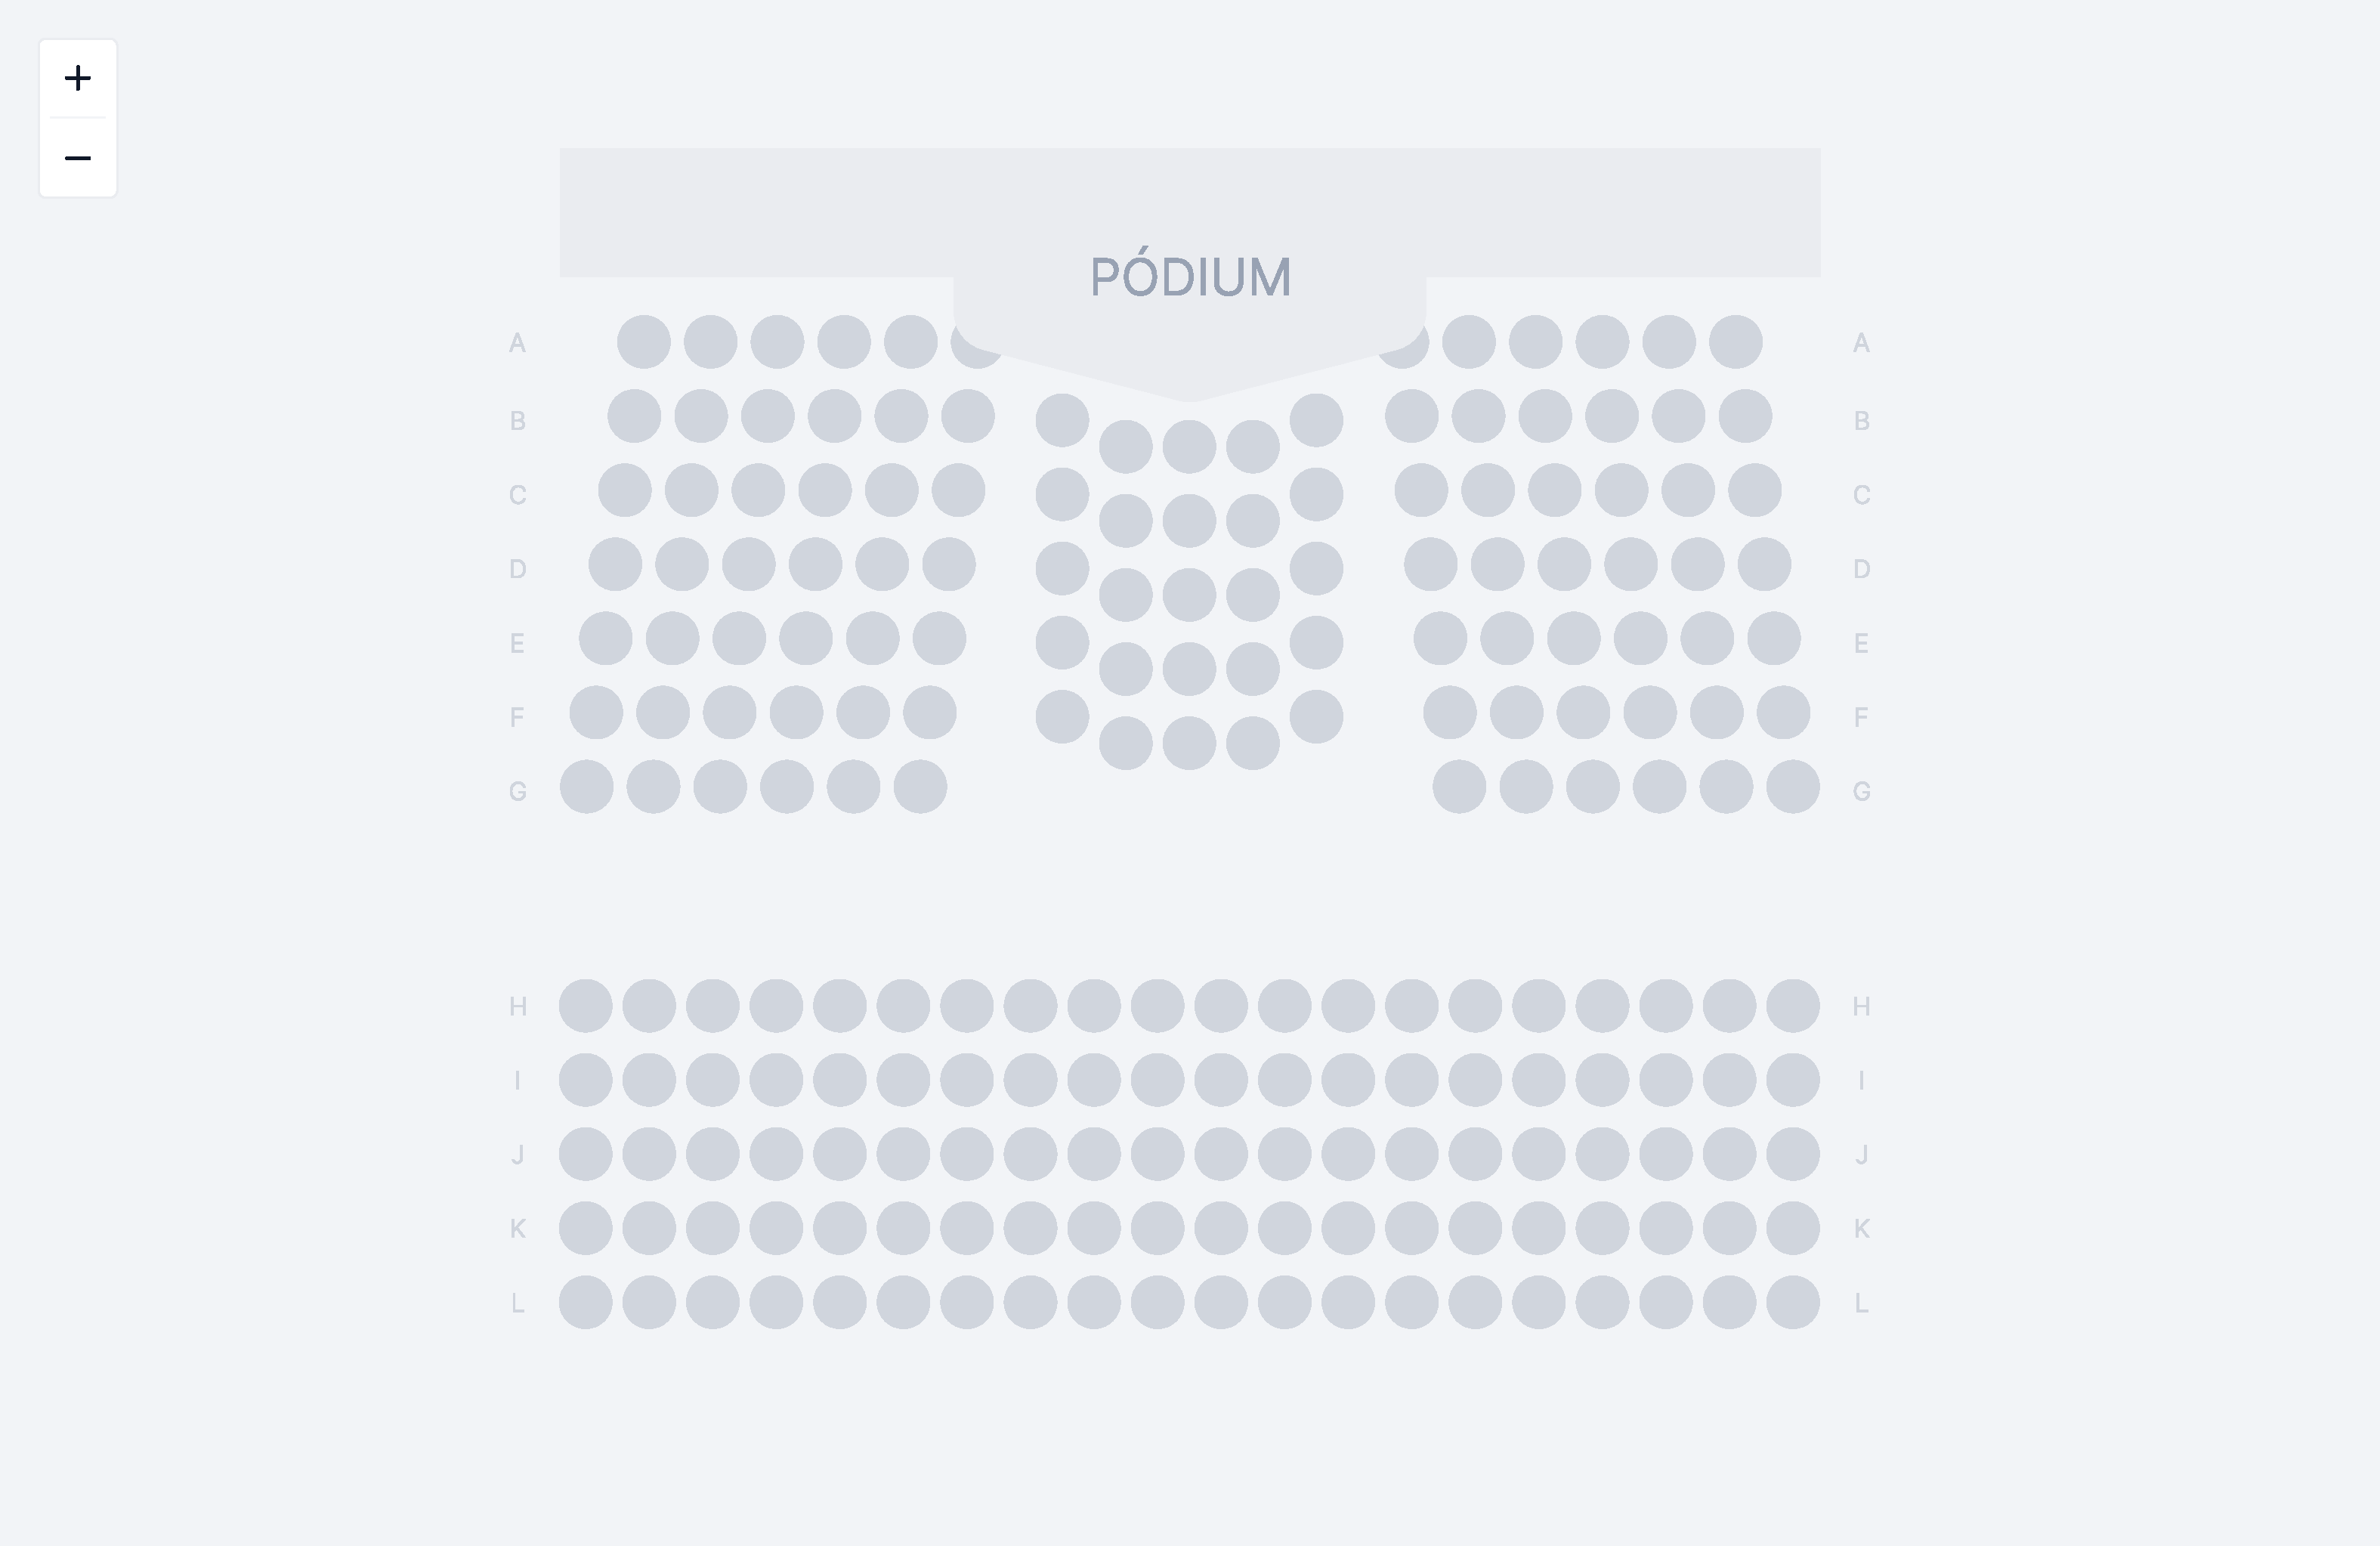
\includegraphics[width=\textwidth]{\FIGDIR/ui/us1-seating-map-desktop-1}
            \label{fig:us1-seating-map-desktop-1}
        \end{subfigure}
        \begin{subfigure}{0.2\textwidth}
            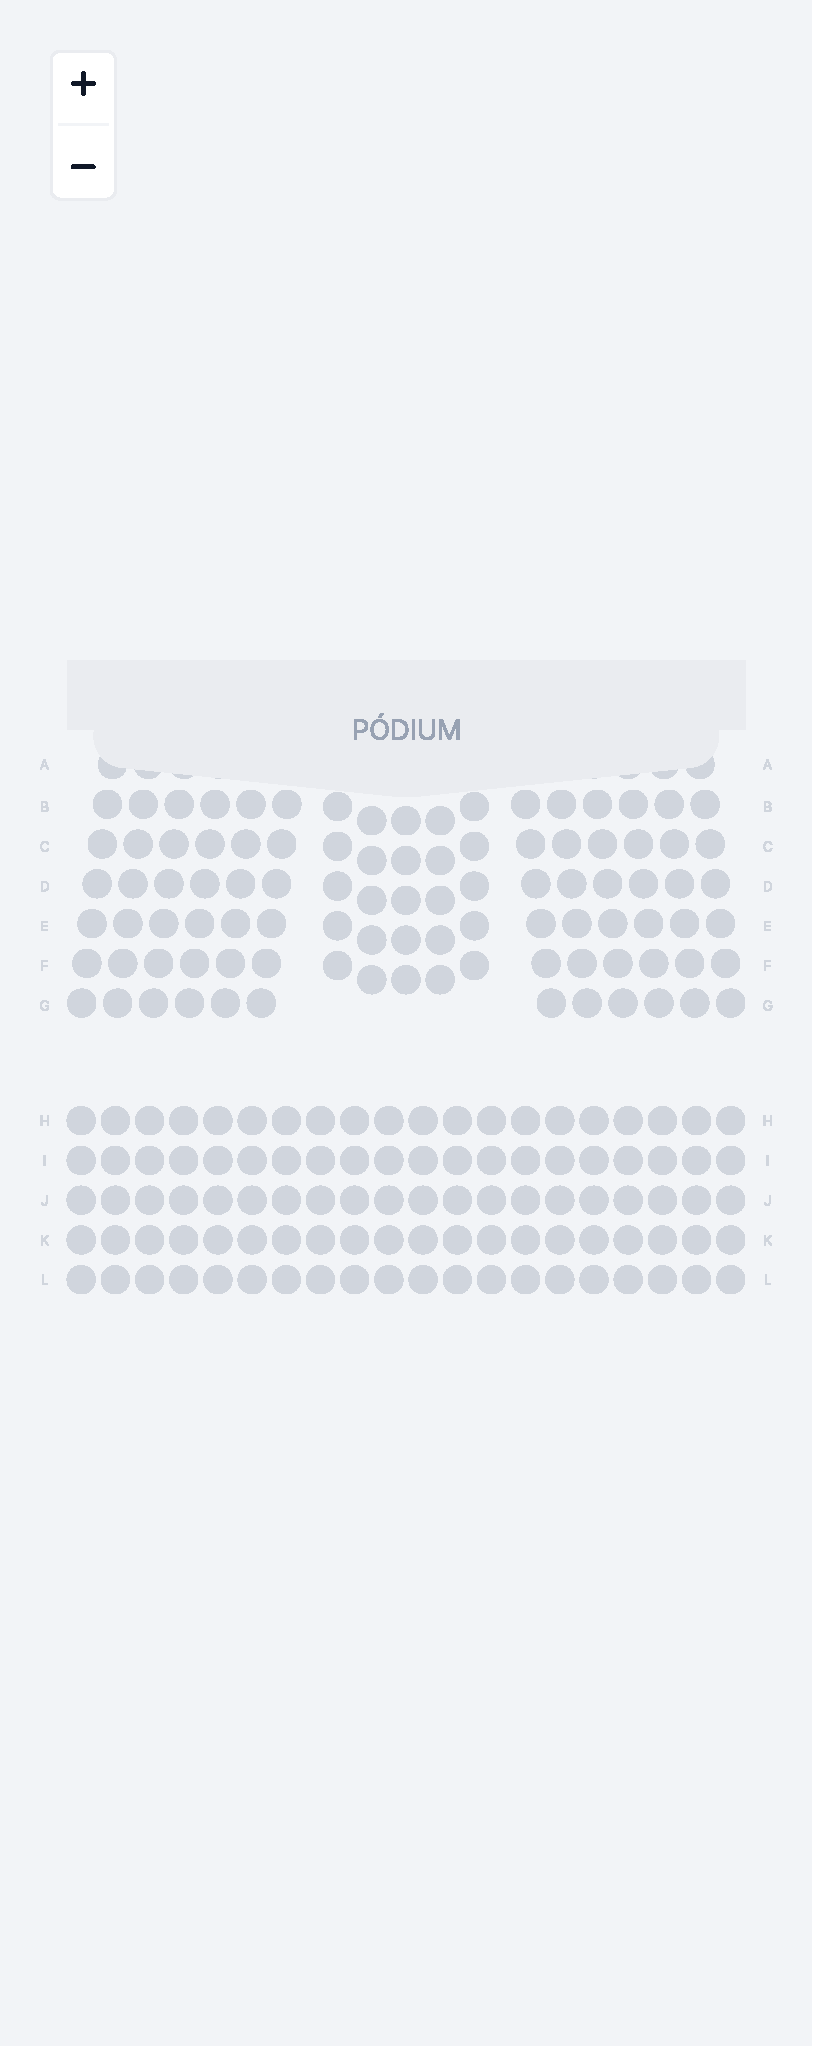
\includegraphics[width=\textwidth]{\FIGDIR/ui/us1-seating-map-mobile-1}
            \label{fig:us1-seating-map-mobile-1}
        \end{subfigure}
        \source
        \label{fig:us1-seating-map}
    \end{figure}

    Na obrázku~\ref{fig:us1-seating-map} je zobrazen návrh komponenty, která by měla být schopna zobrazit plán sedadel místa konání.
    Součástí této komponenty je i boční ovládací panel, které umožňuje manuální přiblížení či oddálení plánu sedadel.
    U této komponenty se předpokládá, že její následná ovladatelnost bude primárně zajištěna pomocí myši, případně pomocí gest na dotykové obrazovce.

\end{subsection}

%%% Podsekce - Výběr sedadel
%%%%% Wording: ✅
%%%%% Styling: ✅
%%%%% References: ✅
%%%%% Grammar: ✅
%%% --------------------------------------------------------------
\begin{subsection}{Výběr sedadel}
    \label{subsec:narvh-ui-transformace-uzivatelskych-pribehu-vyber-sedadel}
    \userstoryseatselection

    Tento uživatelský příběh se zaměřuje na možnost výběru sedadel, která uživatelé chtějí zakoupit.
    Uživatelé by měli mít kontrolu nad výběrem svých sedadel, což implikuje potřebu rozhraní, které nejen zobrazuje plán sedadel, ale také umožňuje interaktivní výběr a zrušení výběru jednotlivých sedadel.

    Praktickým řešením tohoto uživatelského příběhu může být přidání klikacích prvků do plánu sedadel, které budou reprezentovat jednotlivá sedadla.
    Tyto prvky by měly po interakci jasně indikovat stav výběru či zrušení výběru, poskytující uživateli okamžitou vizuální zpětnou vazbu.

    Jakmile je sedadlo vybráno, plán sedadel by měl tuto volbu odrazit změnou barvy sedadla nebo přidáním výrazného značení.
    Stejně tak, pokud je sedadlo zrušeno, mělo by se vrátit do svého původního stavu.
    Tato vizuální zpětná vazba nejen potvrzuje akci uživatele, ale také jim pomáhá sledovat jejich výběry, když se pohybují po místě konání.

    V otázce funkčnosti, je zásadní zajistit, aby proces výběru a zrušení výběru byl intuitivní a bezchybný.
    Pokud je sedadlo již zarezervováno či z jiného důvodu nedostupné, uživatelské rozhraní by mělo zabránit jeho výběru.

    \begin{figure}[H]
        \centering
        \caption{Návrh komponent pro výběr sedadel}
        \begin{subfigure}{0.775\textwidth}
            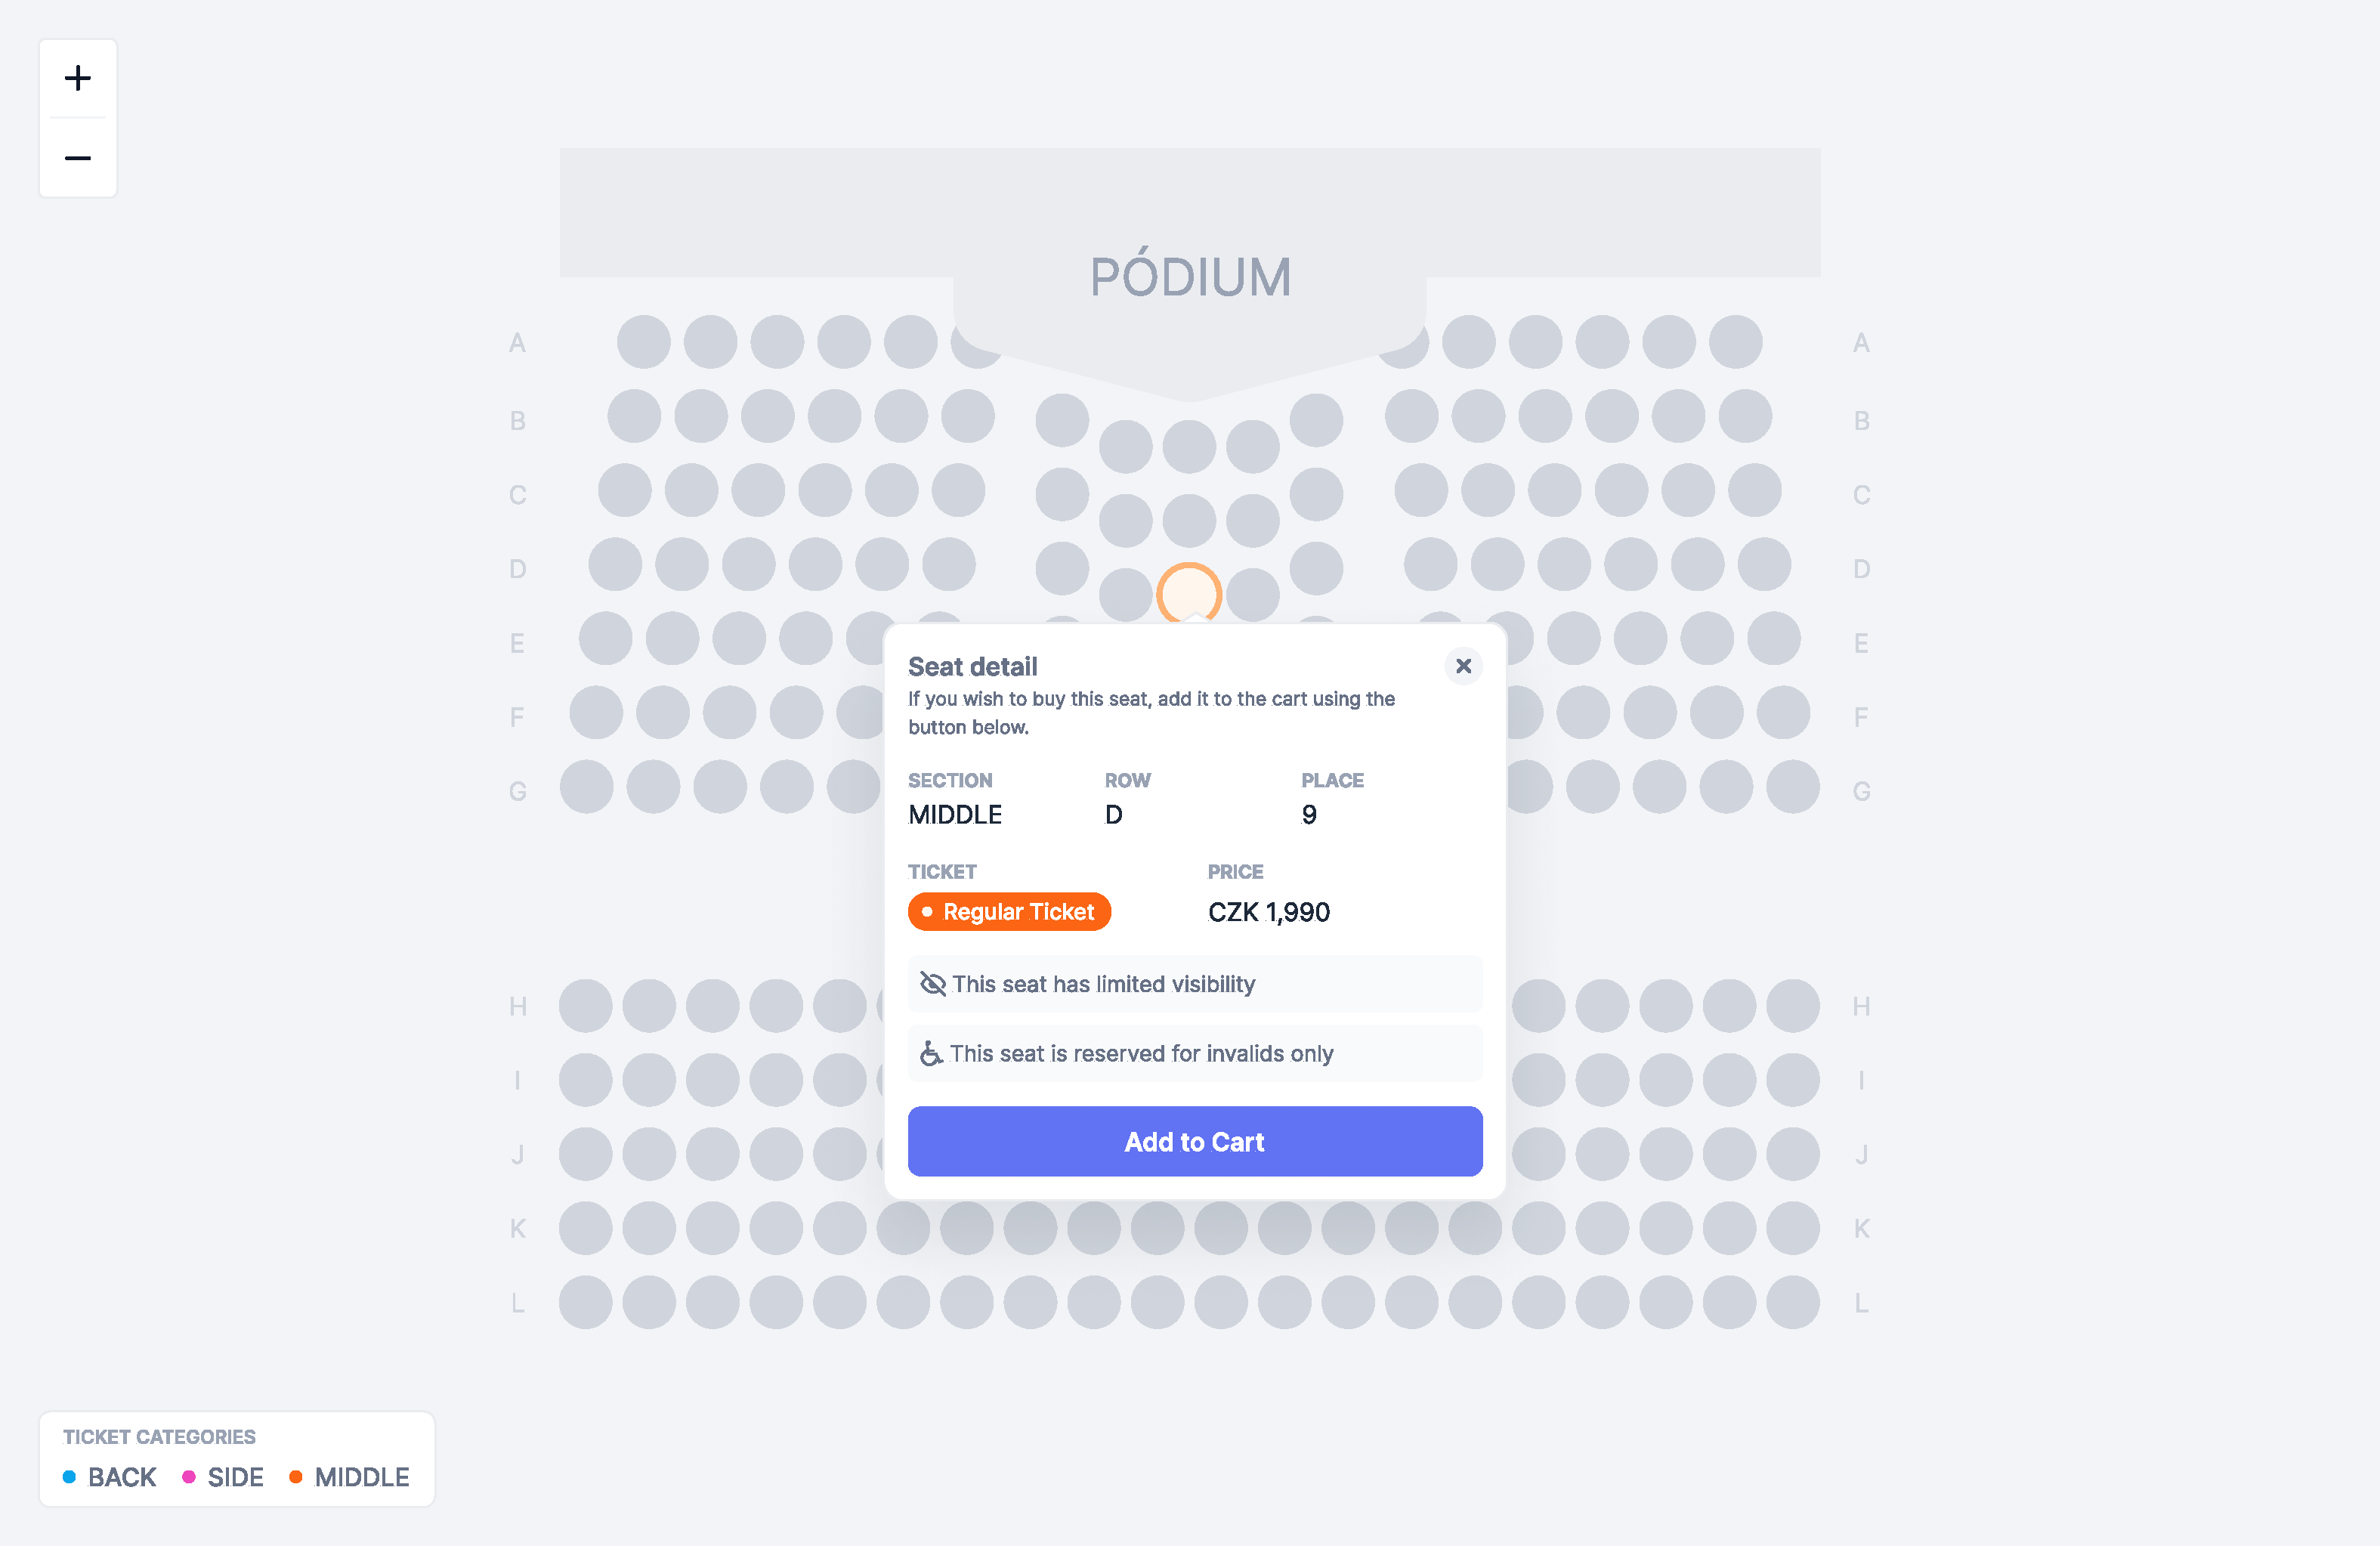
\includegraphics[width=\textwidth]{\FIGDIR/ui/us2-seat-selection-desktop-1}
            \label{fig:us2-seat-selection-desktop-1}
        \end{subfigure}
        \begin{subfigure}{0.2\textwidth}
            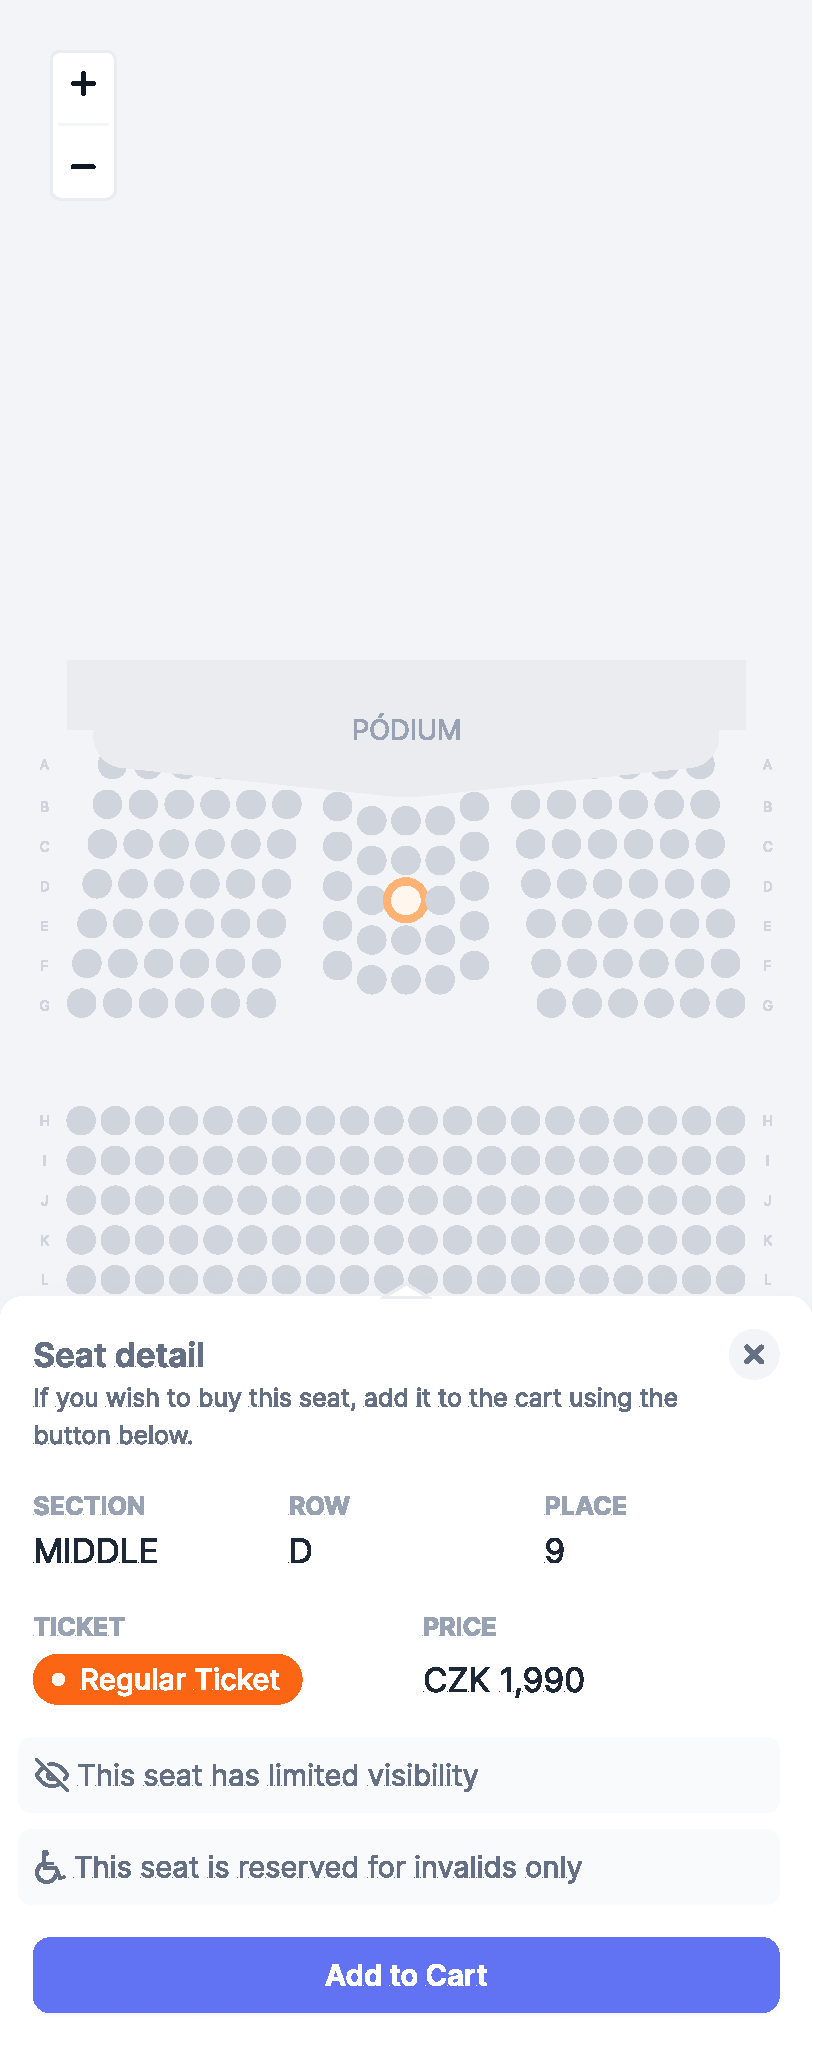
\includegraphics[width=\textwidth]{\FIGDIR/ui/us2-seat-selection-mobile-1}
            \label{fig:us2-seat-selection-mobile-1}
        \end{subfigure}
        \source{}
        \label{fig:us2-seat-selection}
    \end{figure}

    Na obrázku~\ref{fig:us2-seat-selection} je vyobrazen návrh interaktivní komponenty plánu míst, která umožňuje výběr sedadel.
    Volná sedadla k výběru jsou označena výraznými barvami, které odpovídají jejím cenovým kategoriím.
    Tyto kategorie, pro větší přehlednost, jsou zobrazeny v legendě, která je umístěna v pravém dolním rohu komponenty.

    Pro tuto komponentu je zásadní jasně rozpoznat různé stavy sedadel, jako například dostupné, nedostupné, již přidané či aktuálně označené.
    Některé tyto stav mohou být navíc i různě kombinovány, jako například již přidané a aktuálně označené sedadlo.
    Tyto stavy jsou zobrazeny v rámci návrhy komponenty \foreign{Seat} na obrázku~\ref{fig:component-seat} níže.

    \begin{figure}[H]
        \centering
        \caption{Komponenta sedadla a její stavy}
        \includegraphics[width=0.8\textwidth]{\FIGDIR/ui/component-seat}
        \source{}
        \label{fig:component-seat}
    \end{figure}

    Součástí návrhu této komplexní komponenty, ačkoliv není přímo součástí uživatelského příběhu, je i komponenta zobrazující přehledný detail právě vybraného sedadla.
    Sedadla totiž mohou nést různé informace, jako například číslo sedadla, jeho kategorie, cena, či informace o tom, zda je již obsazené nebo má například zhoršenou viditelnost na jeviště.
    Hlavní funkcí této komponenty je potvrzení výběru sedadla, tedy jeho přidání do košíku, či zrušení výběru.
    Na obrázku~\ref{fig:component-seat-} je vyobrazen návrh této komponenty.

    \begin{figure}[H]
        \centering
        \caption{Komponenta detailu zvoleného sedadla}
        \includegraphics[width=\textwidth]{\FIGDIR/ui/component-seat-detail}
        \source{}
        \label{fig:component-seat-}
    \end{figure}

    Tato komponenta funguje jakési modální okno, které se zobrazí po kliknutí na sedadlo.
    Ovšem jeho zobrazení je specifické na desktopové a mobilní verzi, jak je vyobrazeno na obrázku~\ref{fig:us2-seat-selection}.
    Na desktopové verzi se zobrazí jako popover okno umístěné u právě označeného sedadla.
    Na mobilní verzi se toto okno chová jako fixně umístěný list, který se zobrazí v dolní části obrazovky.
    Díky umístění v dolní části obrazovky na mobilních zařízeních se tak zajistí komfortní ovládání a interakce s tímto listem, jelikož se nachází v dosahu palce neboli v tzv. \foreign{thumb zone}.
\end{subsection}
\pagebreak

%%% Podsekce - Nákupní košík
%%%%% Wording: ✅
%%%%% Styling: ✅
%%%%% References: ✅
%%%%% Grammar: ✅
%%% --------------------------------------------------------------
\begin{subsection}{Nákupní košík}
    \label{subsec:narvh-ui-transformace-uzivatelskych-pribehu-nakupni-kosik}
    \userstoryshoppingcart

    Uživatel se nyní již umí pohybovat na mapě místa konání a vybrat si sedadlo, které chce zakoupit.
    Tento uživatelský příběh poukazuje na nutnost jasného přehledu aktuálního stavu nákupního košíku.
    Nákupní košík by měl uživateli sloužit jako přehled přidaných vstupenek s dalšími informacemi, jako například cena, kategorie, či počet vstupenek.
    Nákupní košík by také měl zobrazovat celkovou cenu všech vstupenek, které jsou v něm obsaženy.
    Poskytnutím těchto informací může zákazník potvrdit svůj výběr, sledovat celkovou cenu objednávky a rozhodnout se, zda bude pokračovat v nákupu, či provede úpravy.

    Ačkoliv není v uživatelském příběhu nijak definováno, lze z technických požadavků předpokládat, že celý proces vytváření objednávky bude probíhat v rámci rezervace pro zajištění zaručeného výběru sedadel.
    Tato rezervace bude mít časový limit, po jehož vypršení bude rezervace automaticky zrušena a sedadla budou opět uvolněna k prodeji.
    Tuto informaci je tedy taktéž nezbytné zobrazit ideálně v rámci této komponenty nákupního košíku.
    Tuto komponentu nákupního košíku lze také použít jako navigační prvek, který umožní uživateli přejít k dalším krokům v procesu nákupu.

    Na obrázku~\ref{fig:us3-cart-summary-desktop} je vyobrazen návrh komponenty přehledu nákupního košíku v desktopové verzi.
    Díky velkému prostoru, který je na desktopových zařízených k dispozici, je možné zobrazit všechny informace o vstupenkách, které jsou v košíku obsaženy.
    Tuto komponentu lze vyobrazit jako postranní panel, obsahující všechny tyto informace.
    Díky umístění této komponenty na pravou strany celé obrazovky, kterou pokrývá komponenta mapy sedadel, je zajištěno, že uživatel bude mít vždy přehled o svém výběru, bude jasně viditelný a vyplní zbytečně nevyužitý prostor na obrazovce.

    \begin{figure}[H]
        \centering
        \caption{Návrh komponent přehledu nákupního košíku (desktopová verze)}
        \includegraphics[width=\textwidth]{\FIGDIR/ui/us3-cart-summary-desktop-1}
        \source{}
        \label{fig:us3-cart-summary-desktop}
    \end{figure}

    \pagebreak
    Na mobilní verzi je situace poněkud odlišná.
    V této situaci je k dispozici mnohem méně prostoru, a proto je nutné zobrazit pouze nejdůležitější informace.
    Sekundární informace, jako například cena, či kategorie vstupenky, lze zobrazit například až po rozbalení detailu nákupního košíku.

    \begin{figure}[H]
        \centering
        \caption{Návrh komponent přehledu nákupního košíku (mobilní verze)}
        \begin{subfigure}{0.4\textwidth}
            \includegraphics[width=\textwidth]{\FIGDIR/ui/us3-cart-summary-mobile-1}
            \caption{sbaleno}
            \label{fig:us3-cart-summary-mobile-1}
        \end{subfigure}
        \hfill
        \begin{subfigure}{0.4\textwidth}
            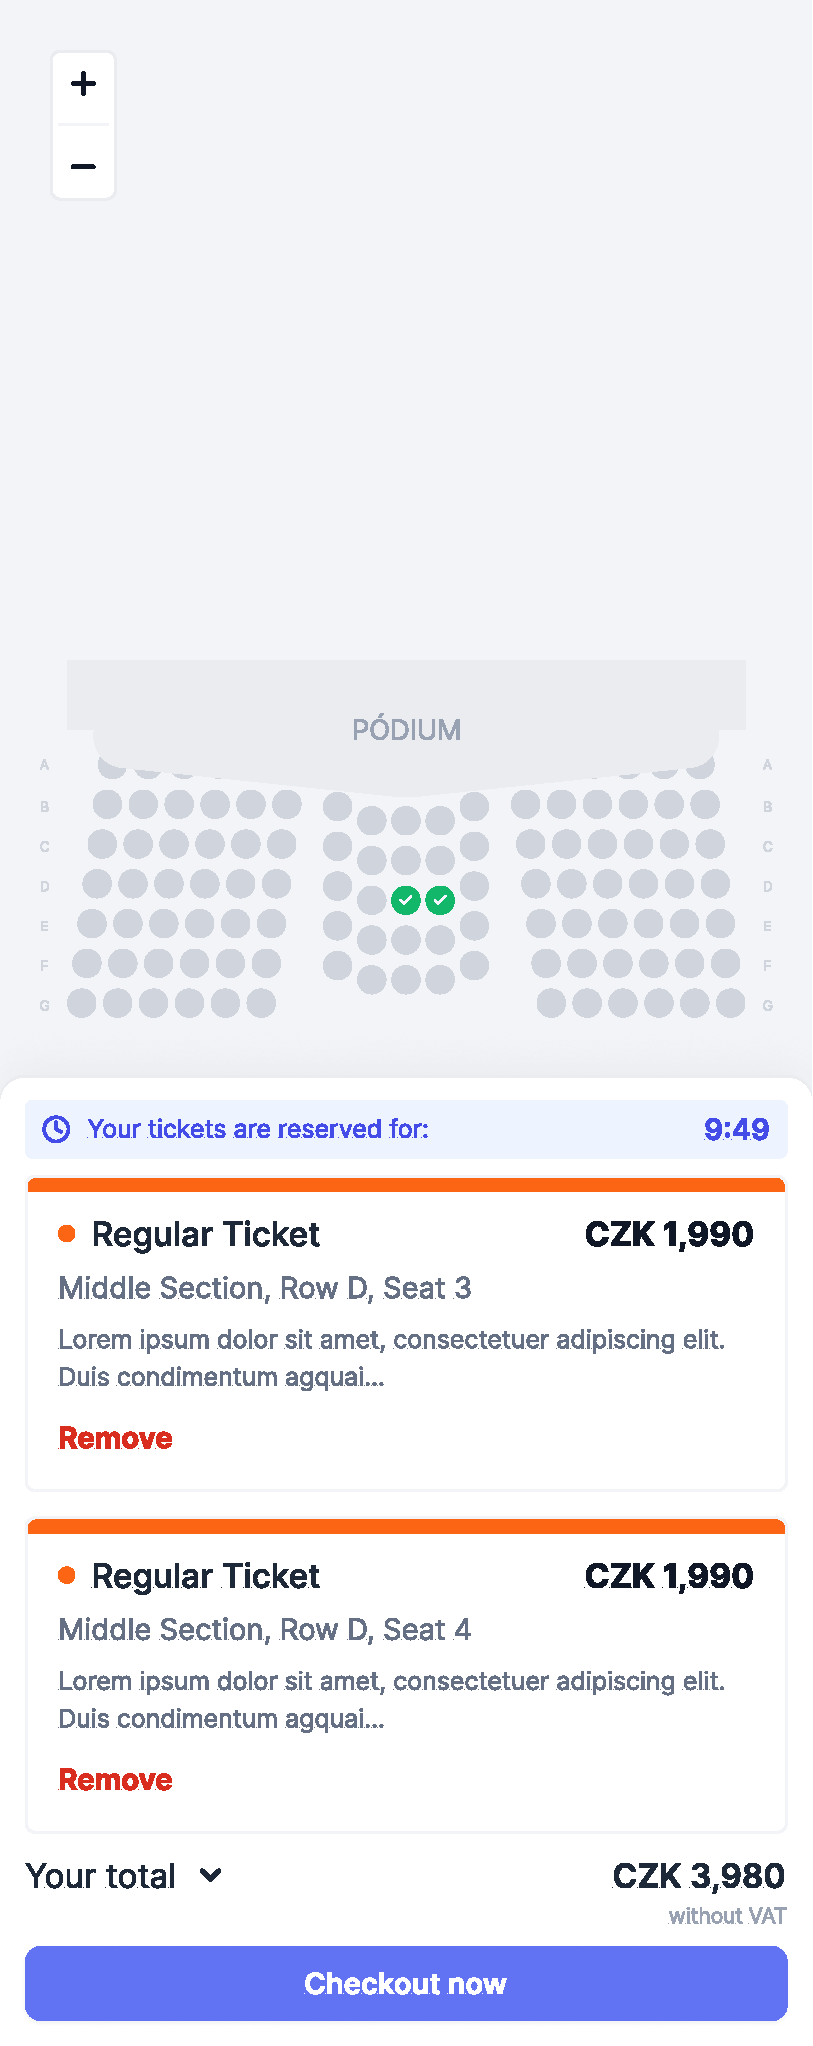
\includegraphics[width=\textwidth]{\FIGDIR/ui/us3-cart-summary-mobile-2}
            \caption{rozbaleno}
            \label{fig:us3-cart-summary-mobile-2}
        \end{subfigure}
        \source{}
        \label{fig:us3-cart-summary-mobile}
    \end{figure}

    Na obrázku~\ref{fig:us3-cart-summary-mobile} je návrh komponenty přehledu nákupního košíku v mobilní verzi, která je umístěna v dolní části obrazovky, aby byla v dosahu palce, a zároveň nezakrývala žádnou důležitou informaci.
    Ve výchozím (sbaleném) stavu obsahuje pouze ty nejdůležitější informace, jako celkovou cenu objednávky.
    Po rozbalení detailu nákupního košíku se zobrazí všechny informace o vstupenkách, které jsou v košíku obsaženy, podobně jako je tomu v desktopové verzi.
\end{subsection}

%%% Podsekce - Vyřízení a potvrzení objednávky
%%%%% Wording: ✅
%%%%% Styling: ✅
%%%%% References: ✅
%%%%% Grammar: ✅
%%% --------------------------------------------------------------
\begin{subsection}{Vyřízení a potvrzení objednávky}
    \label{subsec:narvh-ui-transformace-uzivatelskych-pribehu-vyrideni-a-potvrzeni-objednavky}
    \userstorycheckout

    Proces vyřízení objednávky je posledním krokem v procesu nákupu vstupenek (pokud pomineme krok placení, který není řešen v rámci této práce).
    V tomto kroku je uživatel vyzván k zadání svých osobních údajů, které jsou nutné pro dokončení objednávky.
    Tyto údaje, pro jednoduchost, zahrnují pouze jméno, příjmení, e-mailovou adresu a telefonní kontakt.
    V reálném nasazení by bylo vhodné zahrnout i další údaje, jako například fakturační adresu, či případně další kontaktní údaje.
    Jako speciální údaj lze zákazníkovi nabídnout i možnost vyplnění poznámky k objednávce, která by mohla obsahovat například požadavek na zaslání faktury, či jiné informace.

    Návrh celé této komplexní komponenty je zobrazen na obrázku~\ref{fig:us4-cart-checkout-desktop} níže.
    Tato komponenta, jak je zřejmé, je složena z několika dalších menších částí.

    \begin{figure}[H]
        \centering
        \caption{Návrh komponent dokončení objednávky (desktopová verze)}
        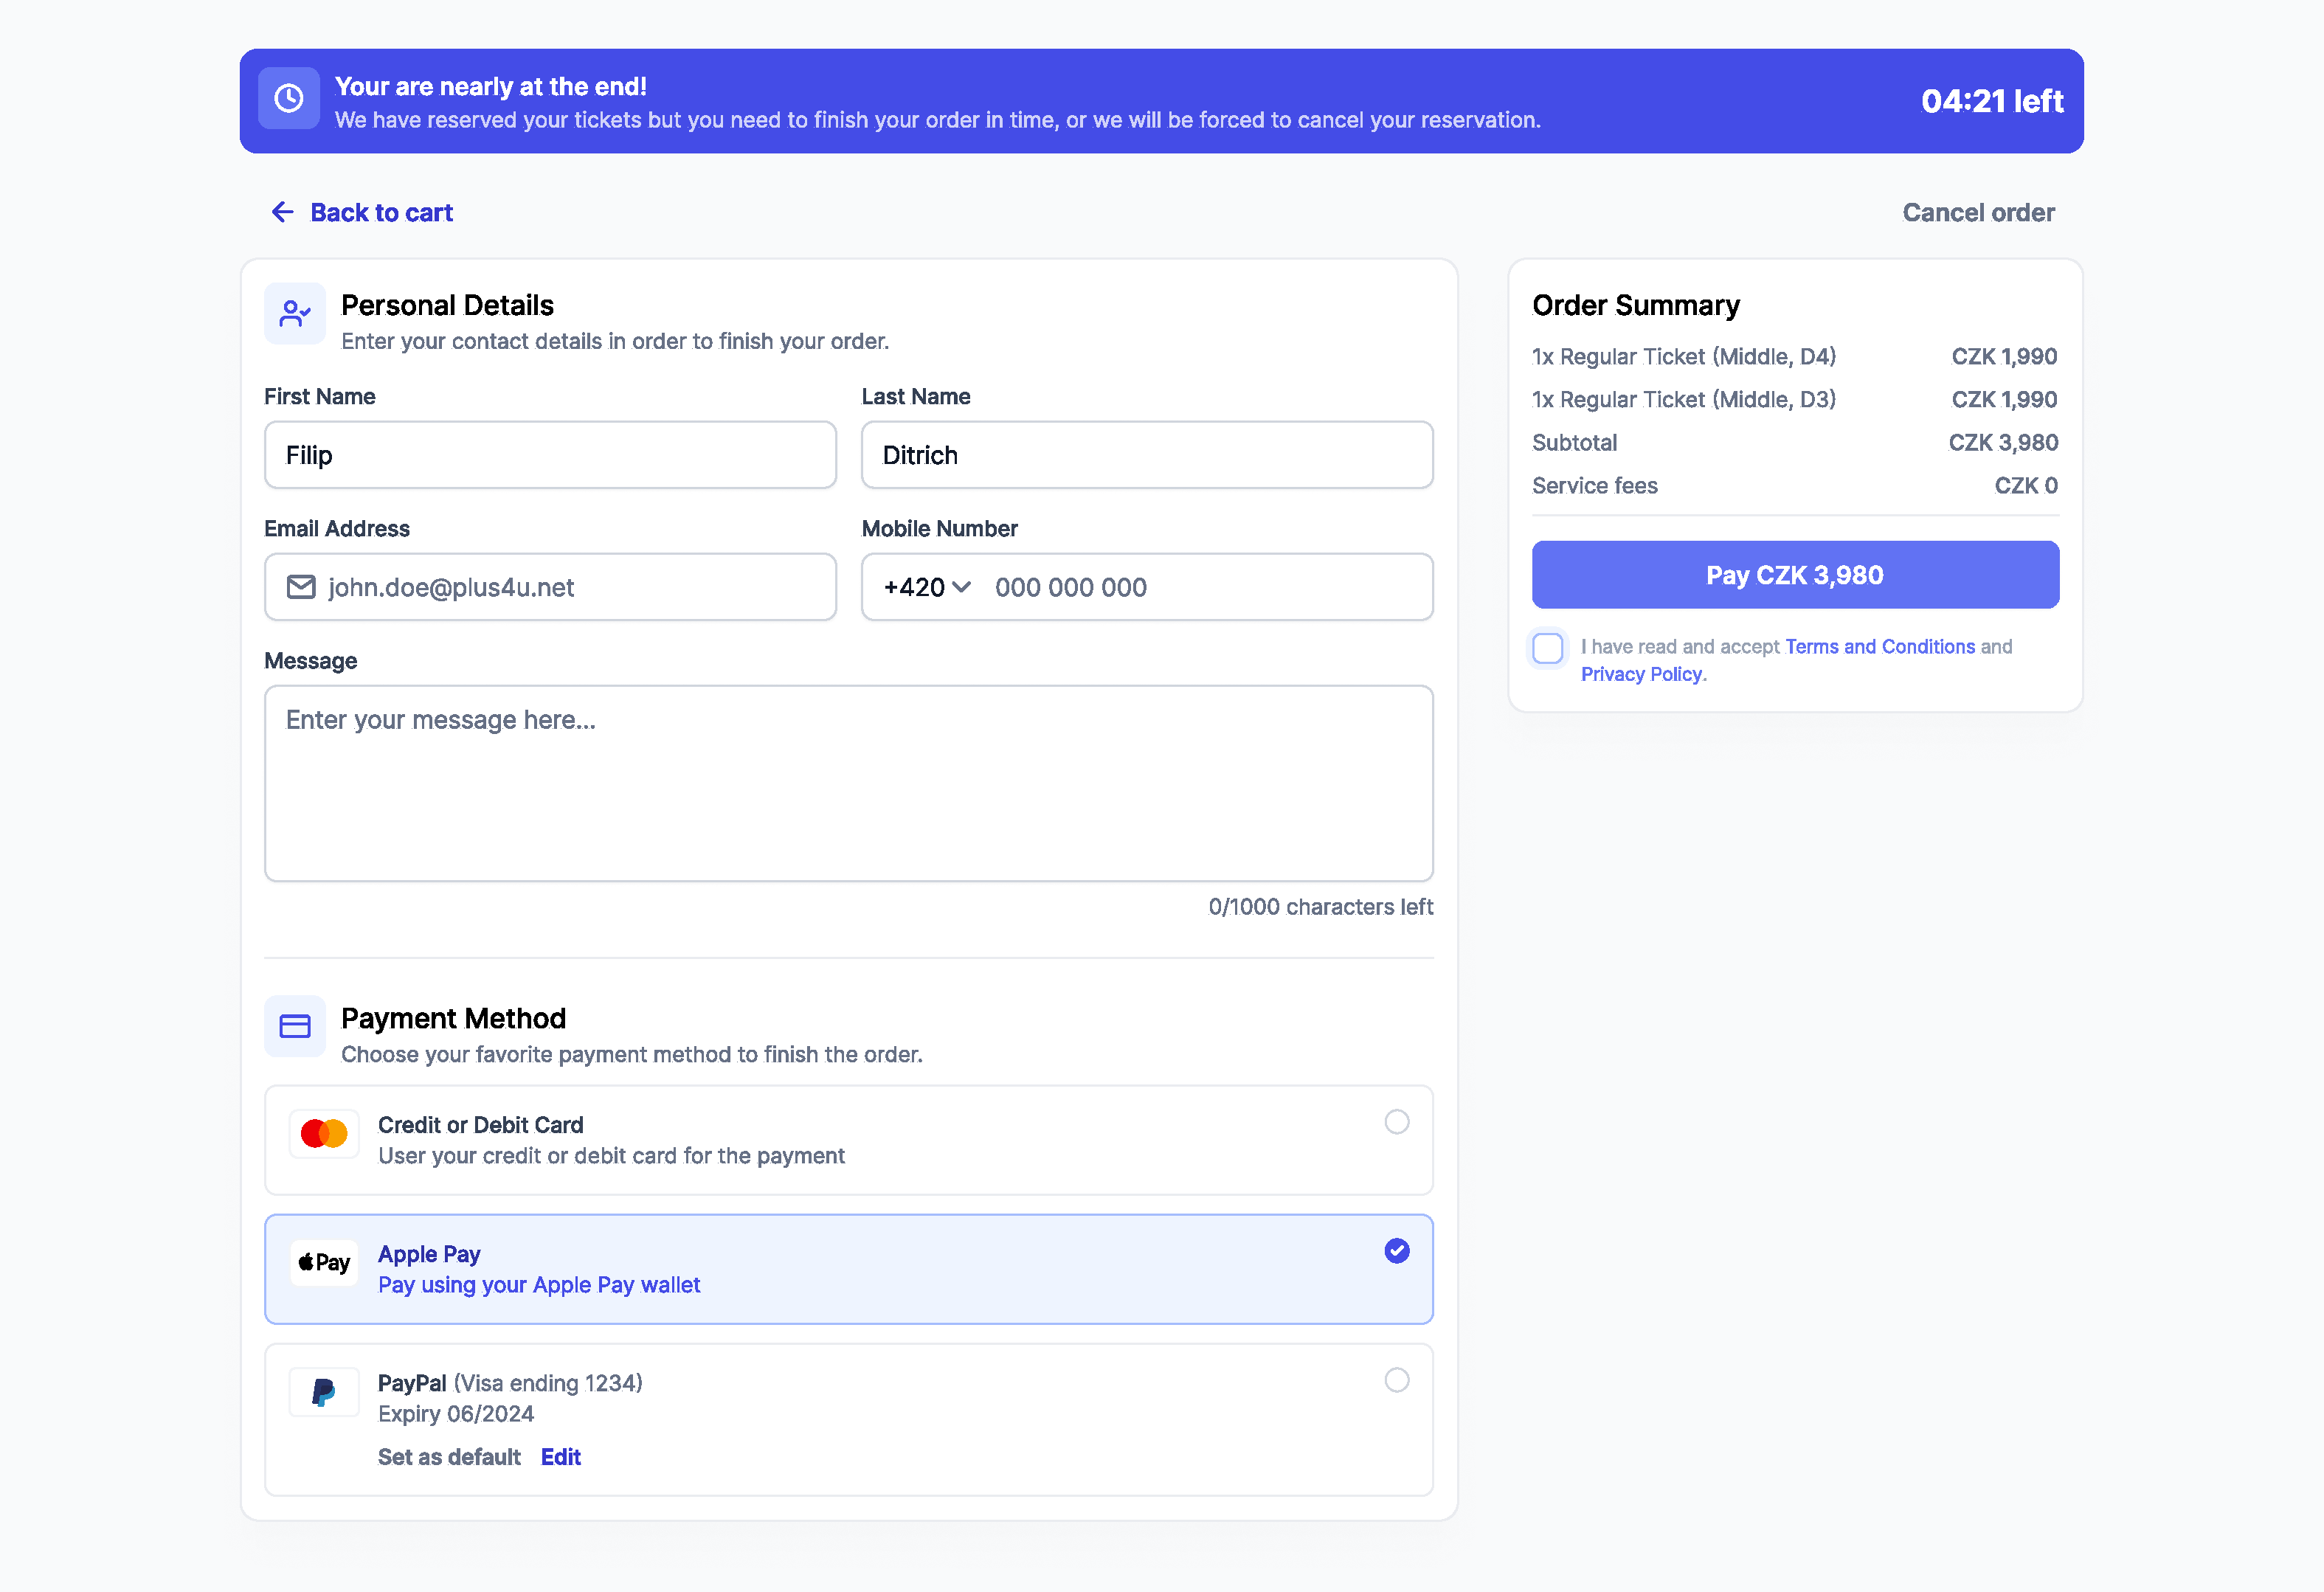
\includegraphics[width=\textwidth]{\FIGDIR/ui/us4-cart-checkout-desktop-1}
        \source{}
        \label{fig:us4-cart-checkout-desktop}
    \end{figure}

    Primární částí je formulář, který obsahuje všechny potřebné údaje pro dokončení objednávky.
    Následuje výběr platební metody a souhrn objednávky, aby měl zákazník stálý přehled o jeho objednávce.
    V neposlední řádě je zde stále zobrazena informace o probíhající rezervaci objednávky a jejím časovém limitu, v rámci, kterého musí zákazník objednávku dokončit, jinak bude rezervace zrušena.
    Dále je zákazníkovi umožněno přejít zpět do procesu výběru vstupenek pomocí tlačítka \foreign{Back to cart} či proces vytváření objednávky kompletně zrušit pomocí tlačítka \foreign{Cancel order}.

    V mobilním rozlišení je zobrazení této komponenty pouze mírně upraveno zarovnáním a umístěním všech prvků do jednoho sloupce, jak je zobrazeno na obrázku~\ref{fig:us4-cart-checkout-mobile} níže.

    \begin{figure}[H]
        \centering
        \caption{Návrh komponent dokončení objednávky (mobilní verze)}
        \begin{subfigure}{0.4\textwidth}
            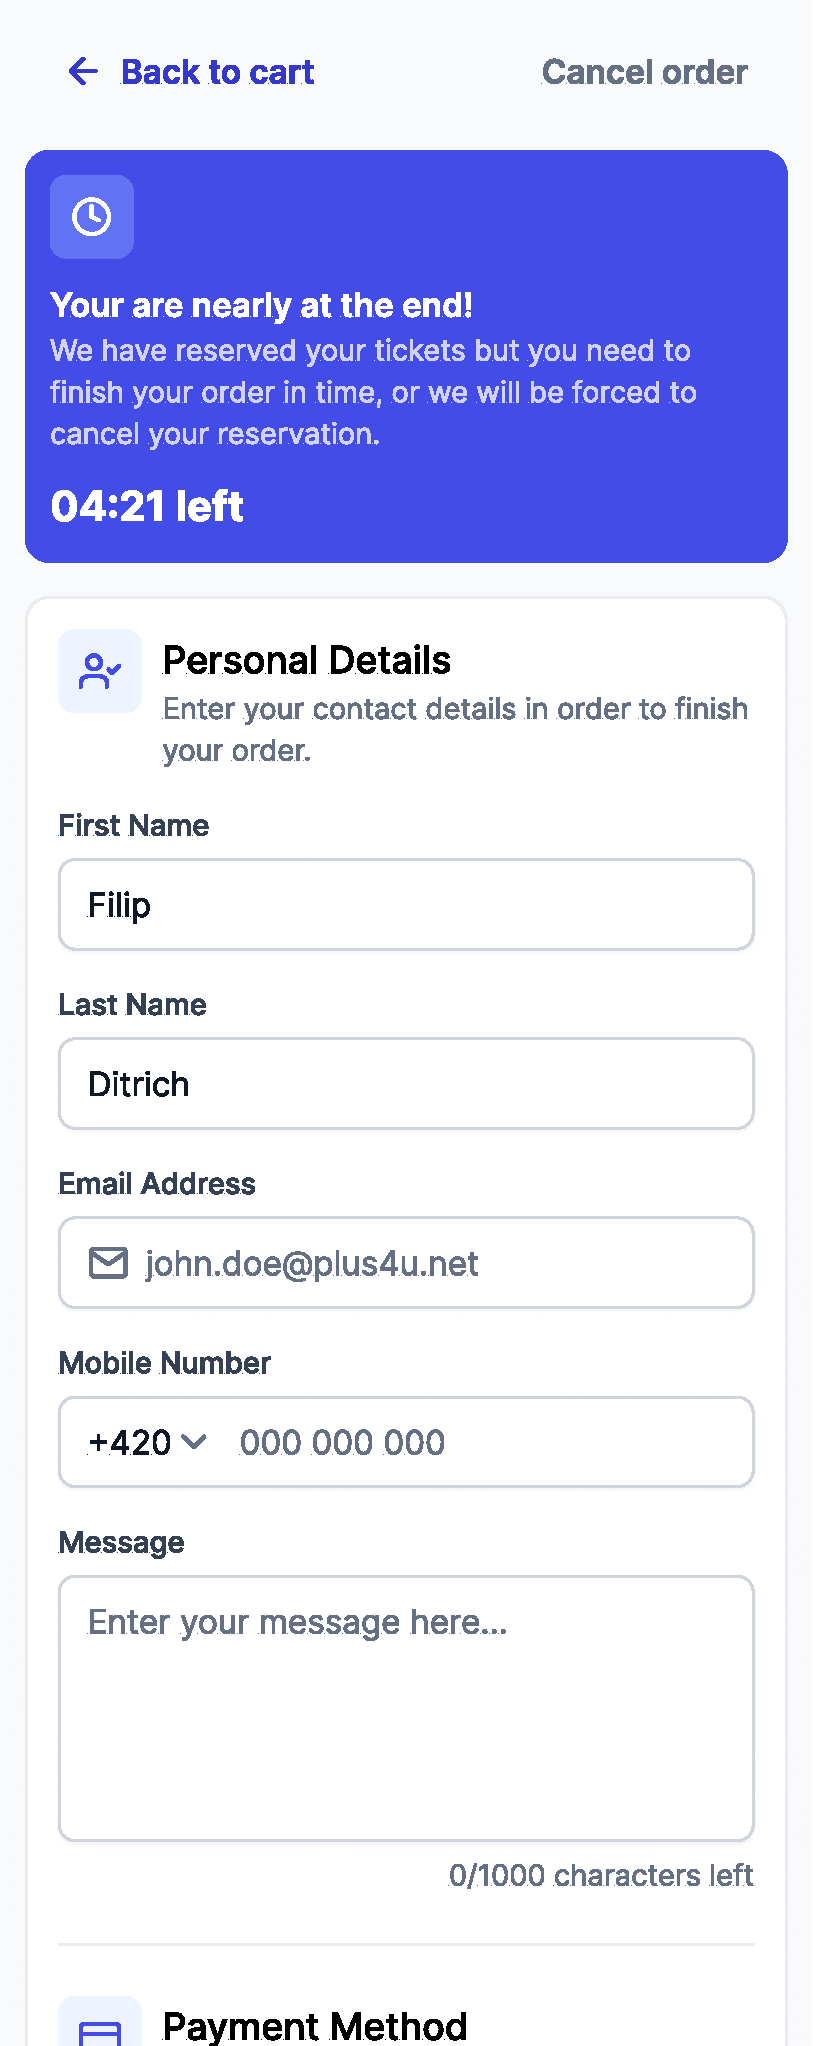
\includegraphics[width=\textwidth]{\FIGDIR/ui/us4-cart-checkout-mobile-1}
            \label{fig:us4-cart-checkout-mobile-1}
        \end{subfigure}
        \hfill
        \begin{subfigure}{0.4\textwidth}
            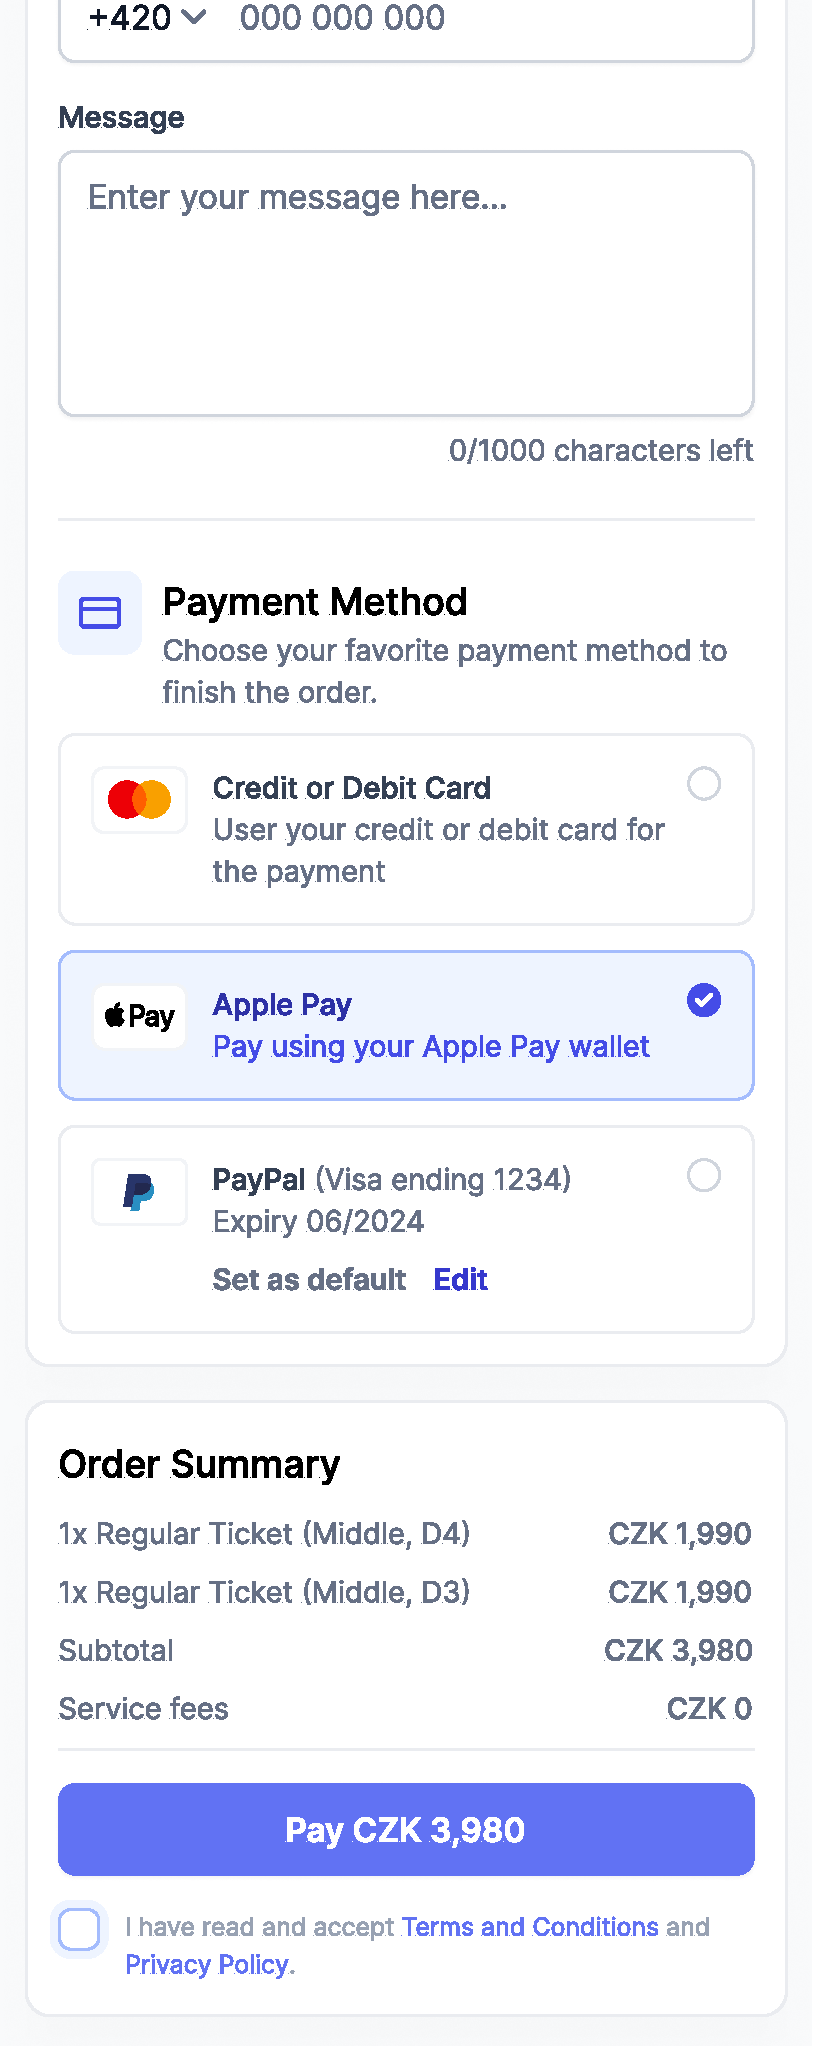
\includegraphics[width=\textwidth]{\FIGDIR/ui/us4-cart-checkout-mobile-2}
            \label{fig:us4-cart-checkout-mobile-2}
        \end{subfigure}

        \source{}
        \label{fig:us4-cart-checkout-mobile}
    \end{figure}

    V obou případech je proces vyřízení objednávky zakončen kliknutím na intuitivní tlačítko \foreign{Pay}.
    Byť není v rámci této práce nutné, v reálném nasazení by bylo nutné vyzvat zákazníka před dokončením objednávky k přečtení a potvrzení obchodních podmínek, případně dalších informací, které by mohly být pro zákazníka důležité.
    Proto je pod tlačítkem dokončení objednávky zobrazeno i povinné zaškrtávací políčko s přijetím obchodních podmínek, jak je zobrazeno na obrázku~\ref{fig:us4-cart-checkout-desktop} výše či v nejspodnější části obrázku~\ref{fig:us4-cart-checkout-mobile}.

    Po kliku na tlačítko dokončení objednávky by byl v reálném světe zákazník přesměrován k zaplacení objednávky, dle jeho zvolené platební metody.
    V rámci této práce je však tento krok zjednodušen a zákazník je přesměrován na stránku s potvrzením dokončení objednávky.

    Tato stránka předpokládá zobrazení informací o zaplacené objednávce a dalšími užitečnými kroky pro zákazníka.
    Vrchní část této komponenty zobrazuje jasné potvrzení o dokončení objednávky a jejím zaplacení spolu s možností stažení PDF souboru s potvrzením o jejím zaplacení, jak je zobrazeno na obrázku~\ref{fig:us4-order-confirmation-desktop} níže.

    \begin{figure}[H]
        \centering
        \caption{Návrh komponent potvrzení objednávky (desktopová verze)}
        \includegraphics[width=\textwidth]{\FIGDIR/ui/us4-order-confirmation-desktop-1}
        \source{}
        \label{fig:us4-order-confirmation-desktop}
    \end{figure}

    Dále je v rámci této komponenty zobrazen přehled dostupných informací o objednávce, jako je například číslo objednávky, datum a čas jejího vytvoření, stav, částka, informace o platbě či seznam zakoupených vstupenek a jejich míst.
    V tomto kroku, byť opět není nutnou součástí zadání této práce, by bylo užitečné zákazníka dále vybídnout k dokončení registrace a vytvoření účtu, aby mohl v budoucnu snadněji sledovat stav svých objednávek a měl přehled o svých vstupenkách.
    Tento krok je naznačen v pravém sloupci na obrázku~\ref{fig:us4-order-confirmation-desktop} výše, kde je zákazník vybídnut k vytvoření hesla pro svůj účet a tím tak vytvoření nového účtu.

    \begin{figure}[H]
        \centering
        \caption{Návrh komponent potvrzení objednávky (mobilní verze)}
        \begin{subfigure}{0.4\textwidth}
            \includegraphics[width=\textwidth]{\FIGDIR/ui/us4-order-confirmation-mobile-1}
            \label{fig:us4-order-confirmation-mobile-1}
        \end{subfigure}
        \hfill
        \begin{subfigure}{0.4\textwidth}
            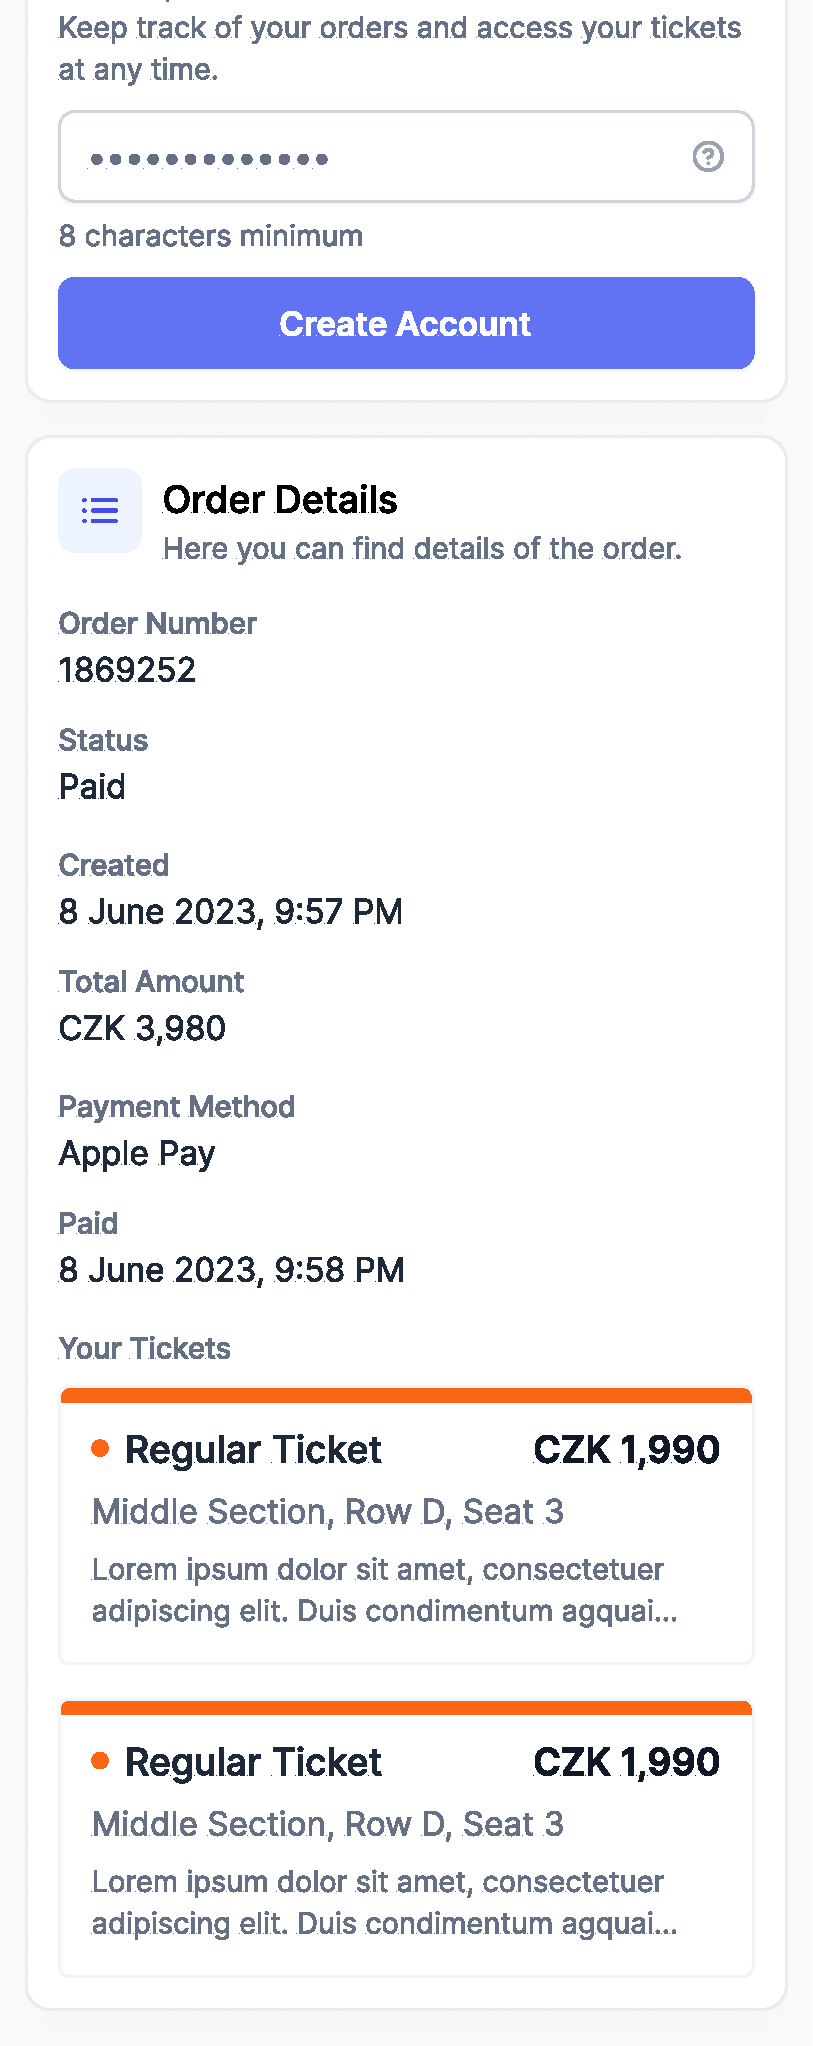
\includegraphics[width=\textwidth]{\FIGDIR/ui/us4-order-confirmation-mobile-2}
            \label{fig:us4-order-confirmation-mobile-2}
        \end{subfigure}
        \source{}
        \label{fig:us4-order-confirmation-mobile}
    \end{figure}

    Mobilní rozložení této komponenty je opět pouze mírně upraveno, aby bylo možné všechny prvky zobrazit v jednom sloupci, jak je zobrazeno na obrázku~\ref{fig:us4-order-confirmation-mobile} výše.

    Tato kapitola vytvořila pevný základ pro pochopení návrhu uživatelského rozhraní, konkrétně v kontextu webového řešení pro prodej vstupenek s rezervací míst.
    To mj.\ zahrnovalo vytvoření uživatelských příběhů, jejich překlad do komponent uživatelského rozhraní a aplikaci efektivních principů návrhu uživatelského rozhraní.
    Dále byl vyzdvihnut výběr nástroje Figma pro návrh toho uživatelského rozhraní.

    V následující kapitole se pozornost přesouvá k implementaci těchto návrhů do funkčního systému prodeje vstupenek s výběrem míst.
\end{subsection}

    % kapitola - implementace
    %%% Kapitola - Implementace aplikace
%%%%% Wording: ⏳
%%%%% Styling: ⏳
%%%%% References: ⏳
%%% --------------------------------------------------------------
\chapter{Implementace aplikace}
\label{ch:implementace}
Vývoj úspěšné webové aplikace zahrnuje orchestraci několika integrovaných aspektů.
Mezi ně patří spojení přitažlivého a intuitivního uživatelského rozhraní (UI) s funkčními požadavky aplikace.
Tato kapitola zkoumá konkrétní procesy, které jsou zapojeny do vývoje frontendu platformy pro prodej vstupenek.

Kapitola objasňuje roli frontendového vývoje a vede skrze racionál za výběrem konkrétních nástrojů a technologií.
Dále se zabývá architektonickým nastavením projektu, vymezuje strukturu projektu a účel za zvoleným uspořádáním.

Ústředním bodem diskurzu jsou jedinečné problémy, které se vyskytly ve fázi implementace.
Mezi ně patří vývoj interaktivního mapování sedadel, správa dynamického nákupního košíku a vytvoření simulovaného backendu a systému pro dokončení objednávky.
Každý z těchto problémů je podrobně popsán a vysvětleny jsou také přístupy k jejich řešení.

Kapitola vyvrcholí komplexní technickou dokumentací finálního produktu, která poskytuje holistické pochopení vyvinuté aplikace.
Podrobný účet slouží nejen k vyprávění o vývojové cestě platformy, ale také k sdílení poznatků o konfrontovaných výzvách a přijatých řešeních.

Prostřednictvím vyváženého vyprávění teoretických základů, praktických aplikací a přístupů k řešení problémů poskytuje tato kapitola neocenitelný zdroj pro ty, kteří se snaží porozumět složitým dynamikám frontendového vývoje webových aplikací.
Následující sekce postupně odhalí podrobné procesy, které přispěly k úspěšnému vývoji platformy pro prodej vstupenek.

    %%% Sekce - Úvod do vývoje frontendu
%%%%% Wording: ⏳
%%%%% Styling: ⏳
%%%%% References: ⏳
%%% --------------------------------------------------------------
\section{Úvod do vývoje frontendu}
\label{sec:implementace-uvod}
Frontendový vývoj, hovorově známý jako vývoj na straně klienta, je nezbytnou součástí vývoje webových aplikací, která se zaměřuje na uživatelské rozhraní a uživatelskou zkušenost.
Týká se všeho, s čím uživatelé vizuálně interagují, včetně návrhu, struktury, chování a obsahu webové aplikace.

Frontend webové aplikace je v zásadě postaven na trojici technologií, a to HTML (HyperText Markup Language), CSS (Cascading Style Sheets) a JavaScript.
HTML strukturuje obsah na webové stránce, CSS jej stylově upravuje a JavaScript jej dělá interaktivní.

Nicméně, oblast frontendového vývoje sahá mnohem dále než tato základní trojice.
V současném vývoji webových aplikací frontendoví vývojáři často využívají sílu pokročilých JavaScriptových knihoven a frameworků, jako jsou React.js, Angular, Vue.js a další, pro vytváření sofistikovaných a interaktivních uživatelských rozhraní.
Kromě toho jsou k dispozici CSS frameworky, jako je Bootstrap nebo Tailwind CSS, které poskytují předdefinované třídy, aby urychlily proces stylování.

Úloha frontendového vývojáře se neomezuje na implementaci návrhů nebo strukturování obsahu; jsou také zodpovědní za to, aby aplikace byla responzivní, výkonná a přístupná.
To znamená, že webová stránka by měla bezchybně fungovat na různých zařízeních s různými velikostmi obrazovek a měla by dodržovat nejlepší postupy v oblasti výkonu, aby poskytovala uživatelům plynulý zážitek.
Kromě toho by aplikace měla být přístupná a měla by uspokojovat uživatele s různými schopnostmi a preferencemi.

Zatímco backendový vývoj se týká serveru a toho, jak aplikace funguje, frontendový vývoj se týká toho, jak aplikace vypadá a jak se uživatel cítí.
Jde o umění a vědu tvorby uživatelsky přívětivého rozhraní, které reaguje na uživatelské interakce intuitivním a angažovaným způsobem.

V následujících sekcích budou představeny a diskutovány konkrétní technologie vybrané pro frontendový vývoj platformy pro prodej vstupenek, přičemž bude osvětlen jejich konkrétní role a důvody jejich výběru.

    %%% Sekce – Výběr technologií
%%%%% Wording: ⏳
%%%%% Styling: ⏳
%%%%% References: ⏳
%%% --------------------------------------------------------------
\section{Výběr technologií}
\label{sec:implementace-techologie}
V této kapitole je zaměření na technologický stack vybraný pro frontendovou implementaci online platformy pro prodej vstupenek.
Tento výběr není náhodný; každá technologie byla vybrána z určitého důvodu, ať už je to kvůli konkrétní funkčnosti, kterou poskytuje, její synergie s ostatními technologiemi ve stacku, nebo kvůli její robustnosti a spolehlivosti.
Následující sekce podrobně popisují každou z těchto technologií.

%%% Podsekce – React.js
%%%%% Wording: ⏳
%%%%% Styling: ⏳
%%%%% References: ⏳
%%% --------------------------------------------------------------
\subsection{React.js}
\label{sec:implementace-techologie-react}
% TODO: open-source footnote explanation
React.js je open-source JavaScriptová knihovna, vyvíjená a udržovaná společností Facebook, která usnadňuje tvorbu uživatelských rozhraní (UI) pro jednostránkové aplikace tím, že umožňuje vývojářům vytvářet znovupoužitelné komponenty uživatelského rozhraní.
Výběr React.js pro tento projekt je ovlivněn několika faktory.

Zaprvé, knihovna se vyznačuje svou funkcí virtuálního DOM, která zvyšuje rychlost a efektivitu vykreslování složitých uživatelských rozhraní.
Virtuální DOM Reactu, na rozdíl od tradičního modelu plného obnovení, umožňuje knihovně minimalizovat přímé manipulace s DOM, což šetří cenný výpočetní čas a zajišťuje plynulejší a výkonnější rozhraní.

Zadruhé, React.js je založen na komponentách, což znamená, že složité uživatelské rozhraní lze rozdělit na menší, znovupoužitelné komponenty.
Tento přístup zvyšuje spravovatelnost kódu a zjednodušuje ladění a testování.
To je zvláště užitečné v kontextu platformy pro prodej vstupenek, kde by několik prvků uživatelského rozhraní mohlo být znovu použito v různých částech aplikace.

Finálně, React.js má silnou podporu komunity, s množstvím zdrojů a nástrojů k dispozici.
Tato podpora je obrovským přínosem při vývoji složitých aplikací a může výrazně snížit čas potřebný k řešení potenciálních problémů.

%%% Podsekce – TypeScript
%%%%% Wording: ⏳
%%%%% Styling: ⏳
%%%%% References: ⏳
%%% --------------------------------------------------------------
\subsection{TypeScript}
\label{sec:implementace-techologie-typescript}
TypeScript je staticky typovaná nadmnožina JavaScriptu, která do jazyka přidává volitelné typy.
TypeScript, vyvinutý a udržovaný společností Microsoft, nejenže zvyšuje schopnosti JavaScriptu, ale také pomáhá při tvorbě aplikací velkého rozsahu s větší spolehlivostí a menší náchylností k chybám.

Zatímco JavaScript je mocný jazyk, často je kritizován pro svou uvolněnost, zejména pokud jde o jeho dynamický typový systém.
TypeScript se snaží tento problém vyřešit tím, že představuje statické typování, což snižuje chyby za běhu a umožňuje lepší vývojové nástroje, jako je automatické dokončování, odvozování typů a typová kontrola.

Jazyk TypeScript se v posledních letech rychle rozšířil a stává se standardem pro vývoj velkých JavaScriptových aplikací.
Pro tento projekt je preferován kvůli jeho větší spolehlivosti a protože dobře spolupracuje s React.js.

%%% Podsekce – Next.js
%%%%% Wording: ⏳
%%%%% Styling: ⏳
%%%%% References: ⏳
%%% --------------------------------------------------------------
\subsection{Next.js}
\label{sec:implementace-techologie-nextjs}
Next.js je open-source React framework, který zjednodušuje proces nastavení a zahrnuje několik užitečných funkcí, jako je server-side rendering a static site generation.
Framework je navržen tak, aby zvýšil výkon a efektivitu React aplikací a vybavil vývojáře nástroji pro tvorbu aplikací s bohatými funkcemi.

V kontextu platformy pro prodej vstupenek byl Next.js vybrán pro své funkce, které zjednodušují běžné úkoly.
Například Next.js má vestavěnou podporu pro API routes, které umožňují vývojářům vytvářet backend API ve stejném repozitáři jako frontend, což je ideální pro simulaci backendové funkcionality.

Next.js dále poskytuje funkce jako routování souborového systému, automatické rozdělení kódu a předvykreslování z krabice, což snižuje množství potřebné konfigurace a nastavení a umožňuje vývojářům soustředit se na logiku aplikace.

%%% Podsekce – Mantine UI
%%%%% Wording: ⏳
%%%%% Styling: ⏳
%%%%% References: ⏳
%%% --------------------------------------------------------------
\subsection{Mantine UI}
\label{sec:implementace-techologie-mantine}
Mantine je komplexní knihovna komponent pro React s důrazem na použitelnost, přístupnost a zkušenosti vývojářů.
Zahrnuje řadu komponent, které lze kombinovat a přizpůsobit k vytvoření složitých a krásných uživatelských rozhraní.
Tato knihovna nabízí jednodušší způsob tvorby uživatelských rozhraní ve srovnání s vytvářením každého komponentu od základů, což může být časově náročné a náchylné k chybám.

Použitím knihovny komponent, jako je Mantine, se zajistí, že komponenty použité v celé aplikaci jsou konzistentní a snižuje se potřeba opakovaného kódu.
Dále se díky důrazu Mantine na přístupnost zajišťuje, že aplikace je použitelná co nejširšímu publiku.

Díky vynikající dokumentaci a bohatému výběru komponentů je Mantine preferovanou volbou pro projekt před jinými knihovnami, jako je MaterialUI.

%%% Podsekce – Tailwind CSS
%%%%% Wording: ⏳
%%%%% Styling: ⏳
%%%%% References: ⏳
%%% --------------------------------------------------------------
\subsection{Tailwind CSS}
\label{sec:implementace-techologie-tailwind}
Tailwind CSS je CSS framework založený na utility-first přístupu pro rychlé vytváření vlastních designů.
Na rozdíl od tradičních CSS frameworků, které poskytují hotové komponenty, umožňuje Tailwind vývojářům vytvářet vlastní designy poskytováním nízkoúrovňových utility tříd, které mohou kombinovat k vytváření jedinečných rozhraní.

V projektu platformy pro prodej vstupenek je Tailwind CSS použit především pro rozložení a rychlé prototypování.
Jeho utility-first přístup zjednodušuje proces tvorby vlastních stylů a jeho responzivní modifikátory umožňují vytvářet designy, které fungují na všech velikostech obrazovky.

%%% Podsekce – Ostatní technologie
%%%%% Wording: ⏳
%%%%% Styling: ⏳
%%%%% References: ⏳
%%% --------------------------------------------------------------
\subsection{Ostatní technologie}
\label{sec:implementace-techologie-ostatni}
Kromě hlavního technologického stacku diskutovaného výše bylo při tvorbě platformy pro prodej vstupenek klíčových několik dalších nástrojů a knihoven.
Každý z nich slouží k jedinečnému účelu a zlepšuje vývojový proces v oblastech jako je kvalita kódu, získávání dat, animace, správa formulářů a pomocné funkce.
Následující sekce popisují každou z těchto kategorií a odpovídající nástroje nebo knihovny použité.

%%% Podpodsekce – Kvalita kódu
%%%%% Wording: ⏳
%%%%% Styling: ⏳
%%%%% References: ⏳
%%% --------------------------------------------------------------
\subsubsection{Kvalita kódu}
\label{sec:implementace-techologie-ostatni-kvalita}
Udržování kvality kódu je klíčové v jakémkoli softwarovém projektu, zejména při práci na komplexních aplikacích.
Vysoká kvalita kódu usnadňuje čtení, údržbu a ladění.
Pro zajištění kvality kódu v tomto projektu byly vybrány dva klíčové nástroje: Prettier a ESLint.

\textbf{Prettier}
Prettier je nástroj pro formátování kódu, který vynucuje konzistentní styl napříč celým kódovým základem tím, že kód analyzuje a znovu jej vytiskne podle svých vlastních pravidel.
Integrací Prettier jsou efektivně eliminovány obavy z formátování kódu.
Nástroj automaticky formátuje kód pokaždé, když je uložen, což zajišťuje, že kódová základna je konzistentní ve stylu, bez ohledu na počet přispěvatelů kódu.
To také pomáhá minimalizovat čas strávený diskutováním a opravováním problémů se stylem.

\textbf{ESLint}
ESLint na druhou stranu je nástroj pro statickou analýzu kódu, který identifikuje problematické vzory v kódu JavaScriptu a TypeScriptu.
Zatímco Prettier se stará o problémy s formátováním, ESLint se zaměřuje na hledání potenciálních chyb a problémů s kvalitou kódu.
Integrací ESLint je možné udržovat kvalitu kódu, čímž se kód stává bezpečnějším a předvídatelnějším.

%%% Podpodsekce – Získávání dat
%%%%% Wording: ⏳
%%%%% Styling: ⏳
%%%%% References: ⏳
%%% --------------------------------------------------------------
\subsubsection{Získávání dat}
\label{sec:implementace-techologie-ostatni-ziskavani}
Získávání dat je kritickým aspektem jakékoliv aplikace, která interaguje se serverem.
V tomto projektu byly pro správu stavu serveru použity Axios a React Query.

\textbf{Axios}
Axios je promise-based HTTP klient pro prohlížeč a Node.js, který zjednodušuje odesílání asynchronních HTTP požadavků na REST koncové body.
S funkcemi jako automatická transformace pro JSON data, ochrana klienta proti XSRF a zpracování požadavků a odpovědí zjednodušuje Axios proces získávání dat v aplikaci.

\textbf{React Query}
React Query je knihovna pro synchronizaci dat pro React, která usnadňuje získávání, cachování a aktualizaci stavu serveru v aplikacích React.
Out-of-the-box se stará o cachování, aktualizace na pozadí a zastaralá data bez nutnosti konfigurace.
Použití s Axios zjednodušuje získávání dat a správu stavu, čímž se snižuje potřeba dalších knihoven pro správu stavu.

%%% Podpodsekce – Animace
%%%%% Wording: ⏳
%%%%% Styling: ⏳
%%%%% References: ⏳
%%% --------------------------------------------------------------
\subsubsection{Animace}
\label{sec:implementace-techologie-ostatni-animace}
Animace přidávají život do aplikací a zlepšují uživatelskou zkušenost.
Pro animace v tomto projektu byly použity Framer Motion a React Spring.

\textbf{Framer Motion}
Framer Motion je produkčně připravená knihovna pro animace v Reactu, která poskytuje intuitivní způsob animace prvků.
Zjednodušuje složité animace a umožňuje vytvářet responzivní animace, které mohou interagovat s gesty uživatele.

\textbf{React Spring}
React Spring na druhou stranu je knihovna pro animace, která využívá fyzikálních principů pro vytváření plynulých a přirozených animací.
Pomocí tzv. springs a dampers animace v React Spring těsně napodobují pohyby ve skutečném světě.

%%% Podpodsekce – Formuláře
%%%%% Wording: ⏳
%%%%% Styling: ⏳
%%%%% References: ⏳
%%% --------------------------------------------------------------
\subsubsection{Formuláře}
\label{sec:implementace-techologie-ostatni-formulare}
Pro správu formulářů v aplikaci byly použity React Hook Form a Zod.

\textbf{React Hook Form}
React Hook Form je knihovna pro správu formulářů v Reactu, která snižuje množství boilerplate kódu potřebného pro vytváření formulářů.
Využitím vestavěných hooků Reactu zjednodušuje React Hook Form validaci formulářů a zlepšuje výkon tím, že minimalizuje počet re-renderů.

\textbf{Zod}
Zod je knihovna pro deklaraci a validaci schémat pro TypeScript a JavaScript.
Použitím s React Hook Form zjednodušuje validaci formulářů a zajišťuje, že data zadaná uživatelem odpovídají definovanému schématu.

%%% Podpodsekce – Pomocné funkce
%%%%% Wording: ⏳
%%%%% Styling: ⏳
%%%%% References: ⏳
%%% --------------------------------------------------------------
\subsubsection{Pomocné funkce}
\label{sec:implementace-techologie-ostatni-pomocne-funkce}
Posledně, Lodash, knihovna pro utility funkce v JavaScriptu, byla použita pro své užitečné funkce jako hluboké klonování objektů, slučování objektů, debouncing a throttling.
To činí kód čistější, čitelnější a udržovatelnější.

Ve shrnutí byly všechny tyto nástroje a knihovny vybrány po pečlivém zvážení jejich funkcí, kompatibility s ostatními částmi technologického stacku a efektivnosti, kterou přinášejí do vývojového procesu.
Hrály významnou roli při vytváření online platformy pro prodej vstupenek a zajistily plynulý a efektivní vývojový proces.

    %%% Sekce – Struktura a architektura projektu
%%%%% Wording: ⏳
%%%%% Styling: ⏳
%%%%% References: ⏳
%%% --------------------------------------------------------------
\section{Struktura a architektura projektu}
\label{sec:implementace-architektura}
Zahájení a strukturování nového projektu je klíčovou fází, která položí základy pro celou aplikaci.
Tato sekce shrnuje proces a úvahy, které jsou zapojeny do počátečního nastavení projektu a definování jeho architektury.
Cílem bylo vytvořit udržitelnou, škálovatelnou a dobře strukturovanou frontendovou aplikaci, která se řídí osvědčenými postupy moderního frontendového vývoje.

%%% Podesekce – Vytvoření projektu
%%%%% Wording: ⏳
%%%%% Styling: ⏳
%%%%% References: ⏳
%%% --------------------------------------------------------------
\subsection{Vytvoření projektu}
\label{subsec:implementace-architektura-vytvoreni-projektu}
Projekt byl vytvoření pomocí příkazu \texttt{create-next-app}, nástroje pro rychlé nastavení nového projektu, který poskytuje Next.js.
Příznak \texttt{--typescript} byl zahrnut, aby bylo jasné, že se má použít TypeScript místo vanilla JavaScriptu.
Tento příkaz vytvoří nový adresář s základní strukturou projektu Next.js a sadou přednastavených souborů.

Jakmile bylo počáteční nastavení projektu dokončeno, následovalo odstranění vygenerovaného boilerplate a přidání vybraných knihoven a technologií pro projekt.
Tento proces zahrnoval odstranění výchozích CSS souborů, protože projekt měl využívat Tailwind CSS pro stylování, a přidání Mantine, komplexní knihovny pro uživatelské rozhraní pro React, a Lodash, knihovny poskytující užitečné funkce pro práci s poli, čísly, objekty, řetězci atd.

Dalším krokem bylo vytvoření zvukové struktury projektu, která vyhovuje potřebám aplikace a podporuje osvědčené postupy.
Dobře promyšlená a organizovaná struktura projektu je zásadní pro udržení čitelnosti kódu, škálovatelnosti a snadné navigace, zejména když kódová základna roste.

Instalace a nastavení dalších knihoven, jako jsou Prettier, ESLint, axios a react-query, byly také součástí této počáteční fáze nastavení.
Tyto nástroje a knihovny dále pomáhají zlepšovat kvalitu kódu, formát, udržovatelnost a pomáhají efektivně zpracovávat volání API\@.

V tomto projektu bylo pro správu balíčků upřednostněno použití \texttt{pnpm}.
Vyniká svým efektivním zacházením s moduly node, čímž zajišťuje rychlejší a spolehlivější sestavení.

Založení nového projektu vyžaduje pečlivé plánování a zvážení budoucích požadavků a rozšíření projektu.
S pevným základem položeným, samotná implementace aplikace se stává plynulejším procesem, jak bude ukázáno v následujících sekcích.

%%% Podesekce – Základní architektura
%%%%% Wording: ⏳
%%%%% Styling: ⏳
%%%%% References: ⏳
%%% --------------------------------------------------------------
\subsection{Základní architektura}
\label{subsec:implementace-architektura-zakladni}
Dobře definovaná struktura projektu je klíčová pro udržitelnost, škálovatelnost a čitelnost kódu.
Logická, jasná a konzistentně udržovaná struktura umožňuje vývojářům snadno procházet a porozumět aplikaci, i když se kódová základna časem rozrůstá a vyvíjí.

Tento projekt následuje modulární architekturu, kde je kód organizován do modulů podle jejich funkcionality.
Tento přístup pomáhá kód učinit čitelnějším a udržovatelnějším tím, že zapouzdřuje související logiku do jednotlivých modulů.

Zde je podrobnější pohled na hlavní adresáře a jejich účely:

\begin{lstlisting}[language={[LaTeX]TeX},caption={Struktura projektu},label={lst:project-structure}]
src/
|-- lib/
|   |-- components/
|   |-- features/
|   |-- graphics/
|   |-- hooks/
|   |-- types/
|   `-- utils/
|-- pages/
`-- styles/
next.config.js
package.json
postcss.config.js
prettier.config.js
tsconfig.json
tailwind.config.js
\end{lstlisting}

\begin{itemize}
    \item \textbf{src:} Toto je hlavní adresář obsahující veškerý zdrojový kód aplikace.
    \item \textbf{src/lib:} Tento adresář obsahuje hlavní funkce projektu, které jsou dále rozděleny do podadresářů:
    \item \textbf{src/lib/components:} Tento adresář obsahuje znovupoužitelné komponenty, jako jsou \textit{DefinitionItem}, \textit{LoadingOverlay} a \textit{TicketCard}, každá ve svém vlastním adresáři se soubory TypeScript a stylování.
    \item \textbf{src/lib/features:} Tento adresář se skládá z konkrétních funkcí nebo logických částí aplikace, jako je klient API, správa košíku, mapování sedadel, správa více pohledů a utility funkce.
    \item \textbf{src/lib/graphics:} Tento adresář uchovává grafické zdroje, jako jsou ikony SVG používané v aplikaci.
    \item \textbf{src/lib/hooks:} Tato složka obsahuje vlastní React hooks, jako jsou \textit{useApiQuery}, \textit{useContextRequired}, \textit{useDebug}, \textit{useHandler} a \textit{useNow}.
    \item \textbf{src/lib/types:} Tento adresář uchovává běžné typy TypeScript používané v celé aplikaci.
    \item \textbf{src/lib/utils:} Tento adresář obsahuje utility funkce používané v aplikaci.
    \item \textbf{src/pages:} Obsahuje komponenty stránek a API endpointy.
    \item \textbf{src/styles:} It includes global styles for the application.
    \item \textbf{src/styles:} Obsahuje globální styly aplikace.
    \item \textbf{next.config.js:} Konfigurační soubor pro Next.js, který umožňuje přizpůsobení různých aspektů frameworku.
    \item \textbf{package.json:} Soubor obsahuje metadata projektu a seznam závislostí použitých v projektu.
    \item \textbf{postcss.config.js, prettier.config.js, tsconfig.json:} Jsou to konfigurační soubory pro PostCSS, Prettier a TypeScript.
    \item \textbf{tailwind.config.js:} Konfigurační soubor pro Tailwind CSS, knihovnu CSS typu utility-first použitou v projektu.
\end{itemize}

Každá z těchto složek a souborů hraje v aplikaci klíčovou roli a přispívá ke struktuře a architektuře projektu.
Použití této konkrétní struktury zajišťuje jasnou oddělenost zájmů, což usnadňuje práci na jednotlivých aspektech projektu, aniž by se ovlivňovaly ostatní.

V dalších sekcích budou podrobněji popsány konkrétní implementační detaily projektu, začínaje interaktivní mapou sedadel.

    %%% Sekce – Interaktivní mapa sedadel
%%%%% Wording: ⏳
%%%%% Styling: ⏳
%%%%% References: ⏳
%%% --------------------------------------------------------------
\section{Interaktivní mapa sedadel}
\label{sec:implementace-seating}
Vývoj webové aplikace zahrnuje několik klíčových prvků, z nichž každý představuje jedinečné výzvy a příležitosti k učení.
Tyto prvky jsou základem funkčnosti aplikace a každý z nich hraje klíčovou roli při zlepšování uživatelské zkušenosti.
Vývoj těchto prvků vyžadoval pevné porozumění frontendovým technologiím, jejich možnostem, omezením a osvědčeným postupům.

Jedním z těchto klíčových prvků je interaktivní mapa sedadel.
Tato funkce umožňuje uživateli vizuálně procházet uspořádáním sedadel v místnosti a vybrat si své preferované místo.
Mapa sedadel uživatelům poskytuje přehled o všech dostupných sedadlech, jejich kategoriích a stavech, čímž usnadňuje proces rozhodování.
Tato funkce výrazně zlepšuje uživatelskou zkušenost tím, že poskytuje intuitivní a interaktivní rozhraní pro výběr sedadel.

%%% Podsekce – Struktura
%%%%% Wording: ⏳
%%%%% Styling: ⏳
%%%%% References: ⏳
%%% --------------------------------------------------------------
\subsection{Struktura}
\label{subsec:implementace-seating-struktura}
Struktura této funkce je postavena na několika komponentech, které spolu harmonicky spolupracují.
Primárními komponentami jsou:

\begin{itemize}
	\item SeatingMapProvider
	\item SeatingMap
	\item VirtualMap
	\item Seat
	\item SeatSheet
\end{itemize}

\textbf{SeatingMapProvider} je nadřazená komponenta, která získává data z API a zpřístupňuje je ostatním komponentám.
Tato data zahrnují podrobnosti o místnosti, sedadlech, jejich stavech a přidružených vstupenkách.

\textbf{SeatingMap} je komponenta, která zpracovává SVG data.
Přebírá SVG data z API a překládá je do formátu, který může být použit komponentou VirtualMap.

\textbf{VirtualMap} je zodpovědná za přidání interaktivity do SeatingMap.
Umožňuje funkce, jako je posouvání, přibližování a oddalování mapy, čímž poskytuje dynamický uživatelský zážitek.

\textbf{Seat} a \textbf{SeatSheet} komponenty představují jednotlivá sedadla na mapě a podrobnosti zobrazené při výběru sedadla.

\begin{minted}[breaklines]{jsx}
<SeatingMapProvider venue={venue}>
	{/* seating map */}
	<SeatingMap width={width} height={height}>
		{/* virtual map */}
		<VirtualMap minScaleFactor={1.1} maxScaleFactor={0.1}>
			{/* individual seats */}
			<Seat />
			<Seat />
			<Seat />
			{/* + any other svg elements */}
		</VirtualMap>

		{/* seat sheet detail */}
		<Sheet>
			<Sheet.Header />
			<Sheet.Body>
				<SeatSheetDetail />
			</Sheet.Body>
		</Sheet>
	</SeatingMap>
</SeatingMapProvider>
\end{minted}

%%% Podsekce – Získávání a správa dat
%%%%% Wording: ⏳
%%%%% Styling: ⏳
%%%%% References: ⏳
%%% --------------------------------------------------------------
\subsection{Získávání a správa dat}
\label{subsec:implementace-seating-data}
Proces získávání a správy dat začíná komponentou SeatingMapProvider.
Tato komponenta vytvoří požadavek na API, aby získala data týkající se uspořádání sedadel v místnosti.

\begin{minted}[breaklines]{typescript}
/**
 * Venue API response schema
 * @export
 */
export const venueApiSchema = z.object({
	/** venue id */
	venueId: z.string().uuid(),
	/** venue name */
	name: z.string(),
	/** seating drawing (SVG) */
	drawing: z.string(),
	/** venue seat data */
	seats: z.array(
		z.object({
			/** seat id */
			seatId: z.string().uuid(),
			/** seat row display label */
			row: z.string(),
			/** seat place number */
			place: z.number(),
			/** seat full display name label */
			fullName: z.string(),
			/** seat available capacity left */
			capacityLeft: z.number(),
			tickets: z.array(z.string().uuid()),
			categoryId: z.string().uuid(),
		}),
	),
	/** venue ticket data */
	tickets: z.array(
		z.object({
			/** ticket id */
			ticketId: z.string().uuid(),
			name: z.string(),
			description: z.string().optional(),
			price: z.number().int(),
			categories: z.array(
				z.object({
					categoryId: z.string().uuid(),
					price: z.number().int(),
				}),
			),
		}),
	),
	/** venue ticket categories */
	categories: z.array(
		z.object({
			/** category id */
			categoryId: z.string().uuid(),
			name: z.string(),
			description: z.string().optional(),
			color: z.string(),
		}),
	),
});
\end{minted}

Odpověď API zahrnuje podrobnou SVG reprezentaci uspořádání sedadel v místnosti, jednotlivá data sedadel a přidružené vstupenky.
Každé sedadlo obsahuje informace o jeho řádku, místě, plném názvu, dostupné kapacitě a přidružených vstupenkách a kategoriích.
Každá vstupenka obsahuje informace o jejím id, názvu, volitelném popisu, ceně a kategoriích.

Po získání dat komponenta SeatingMapProvider zpracuje data do použitelnějšího formátu.
Toto zpracování zahrnuje oddělení sedadel, vstupenek a kategorií do vlastních struktur, vytvářející hierarchii, která zjednodušuje přístup k datům pro následující komponenty.

Tento zpracovaný formát je pak ostatním komponentám zpřístupněn pomocí kontextu, což poskytuje pohodlný způsob, jak k nim přistupovat.

%%% Podsekce – Parsování SVG a mapování sedadel
%%%%% Wording: ⏳
%%%%% Styling: ⏳
%%%%% References: ⏳
%%% --------------------------------------------------------------
\subsection{Parsování SVG a mapování sedadel}
\label{subsec:implementace-seating-svg}
SeatingMap komponenta je zodpovědná za parsování SVG dat a jejich překlad do formátu, který může být použit komponentou VirtualMap.

Tato komponenta přijímá SVG data z API a zpracovává je pomocí knihovny xml-js.
SVG data z API následují specifickou strukturu, kde "<g>" elementy představují skupiny sedadel, a tyto jsou identifikovány pomocí id atributu "seats:xxx".
Jednotlivá sedadla v rámci těchto skupin jsou reprezentována "<circle>" elementy, identifikovanými jejich jedinečnými id ve formě "seat:row+place".

% FIXME: svg comments broken
\begin{minted}{xml}
<svg width="1287" height="1115" viewBox="0 0 1287 1115" fill="#F2F4F7" xmlns="http://www.w3.org/2000/svg">
    <!-- seats -->
    <g id="seats:back">
        <!-- seat H+1 -->
        <circle id="seat:H+1" cx="48" cy="785" r="50" fill="#D0D5DD"/>
        <!-- seat I+1 -->
        <circle id="seat:I+1" cx="48" cy="805" r="50" fill="#D0D5DD"/>
        <!-- ...
-->
    </g>
    <g id="seats:right">
        <!-- ...
-->
    </g>
    <g id="seats:left">
        <!-- ...
-->
    </g>
    <g id="seats:center">
        <!-- ...
-->
    </g>
    <!-- details -->
    <g id="details:patio">
        <!-- ...
-->
    </g>
    <!-- ...
-->
</svg>
\end{minted}

Jakmile jsou SVG data zparsována, komponenta SeatingMap mapuje data sedadel na parsované SVG elementy, nahrazující každý "<circle>" element odpovídající komponentou <Seat>.
Každá komponenta <Seat> reprezentuje jedno sedadlo a zahrnuje všechna příslušná data pro toto sedadlo.

%%% Podsekce – Interaktivita s VirtualMap
%%%%% Wording: ⏳
%%%%% Styling: ⏳
%%%%% References: ⏳
%%% --------------------------------------------------------------
\subsection{Interaktivita s VirtualMap}
\label{subsec:implementace-seating-virtualmap}
Komponenta VirtualMap přidává interaktivitu do mapy sedadel.
Tato komponenta obaluje komponentu SeatingMap, přebírající parsované a namapované SVG elementy jako své potomky, a zajišťuje všechny interakce s mapou sedadel.


Tato komponenta využívá knihovny react-spring a use-gesture k implementaci interakcí s mapou sedadel.
Tyto knihovny umožňují plynulé a responzivní animace pro gesta panningu, zoomování a pinching, poskytující dynamický a plynulý uživatelský zážitek.

Komponenta VirtualMap také zajišťuje správu stavu mapy sedadel, sledováním změn, jako je úroveň zoomu, posunutí pan, a aktuálně vybrané sedadlo.
Tato správa stavu zajišťuje konzistentní uživatelský zážitek, i když je mapa sedadel manipulována uživatelem.

%%% Podsekce – Výběr sedadla a správa vstupenek
%%%%% Wording: ⏳
%%%%% Styling: ⏳
%%%%% References: ⏳
%%% --------------------------------------------------------------
\subsection{Výběr sedadla a správa vstupenek}
\label{subsec:implementace-seating-seat}
Komponenta Seat a SeatSheet jsou zodpovědné za výběr sedadla a správu vstupenek.

Komponenta Seat reprezentuje jednotlivá sedadla na mapě.
Každá komponenta Seat zahrnuje všechna příslušná data sedadla, jako je jeho dostupnost a aktuální stav.
Kliknutím na dostupné sedadlo můžou uživatelé zobrazit jeho detaily, včetně příslušných vstupenek.
Tato interakce spouští otevření komponenty SeatSheet, která poskytuje uživatelsky přívětivé rozhraní pro výběr vstupenky.

% TODO: screenshot of the Seat component
\begin{verbatim}
// TODO: screenshot of the SeatSheet component
\end{verbatim}

Komponenta SeatSheet zobrazuje detaily vybraného sedadla, včetně jeho kategorie, řádku, místa a dostupných vstupenek.
Vstupenky jsou vázány na kategorii sedadla a kategorie může mít několik příslušných vstupenek.
Cena vstupenky je definována kombinací její kategorie a vybraného sedadla.

Uživatel může přidat vybranou vstupenku do svého košíku přímo z rozhraní SeatSheet.
Pokud je v košíku již vstupenka pro vybrané sedadlo, může uživatel vybrat, zda chce vstupenku vyměnit nebo ji z košíku odebrat.
Všechny tyto změny se okamžitě promítají do komponenty SeatSheet, poskytující uživateli zpětnou vazbu v reálném čase.

Ve shrnutí je komponenta Interactive Seating Map kombinací načítání a správy dat, parsování SVG a mapování sedadel, interaktivity s VirtualMap a výběru sedadla a správy vstupenek.
Tyto komponenty spolupracují na vytvoření dynamické, interaktivní a uživatelsky přívětivé volby sedadel.
Výsledkem je vysoce flexibilní a intuitivní systém, který zjednodušuje proces výběru vstupenek a správu košíku.

\begin{figure}[h]
	\centering
	\includegraphics[width=\textwidth]{\FIGDIR/seating-map-seat}
	\caption{Snímek obrazovky interaktivní mapy sedadel}
	\label{fig:seating-map-seat}
\end{figure}

Obrázek~\ref{fig:seating-map-seat} zobrazuje výsledný produkt, ilustrující uživatelsky přívětivé rozhraní a dynamickou mapu sedadel.
Kombinace výše uvedených komponent umožňuje snadnou navigaci sedadel místa, okamžitý přístup k informacím o vstupenkách a přehlednou správu vstupenek, což vede k efektivnímu a příjemnému uživatelskému zážitku.

    %%% Sekce – Správa nákupního košíku
%%%%% Wording: ⏳
%%%%% Styling: ⏳
%%%%% References: ⏳
%%% --------------------------------------------------------------
\section{Správa košíku}
\label{sec:implementace-kosik}
Druhou hlavní funkcí naší aplikace je správa košíku.
Tato komponenta umožňuje uživatelům přidávat, odebírat nebo vyměňovat vstupenky, které si vybrali z mapy sedadel, a slouží jako most mezi interaktivní mapou sedadel a procesem rezervace a platby.
Správa košíku je pro aplikaci klíčová, protože ovládá tok dat od výběru sedadel po proces rezervace a platby.

%%% Podsekce – Kontext košíku
%%%%% Wording: ⏳
%%%%% Styling: ⏳
%%%%% References: ⏳
%%% --------------------------------------------------------------
\subsection{Kontext košíku}
\label{subsec:implementace-kosik-kontext}
State košíku je spravován globálně v celé aplikaci pomocí React kontextu.
Definovali jsme \texttt{CartContext}, který obaluje celou aplikaci a poskytuje kontext pro přístup a manipulaci se stavem košíku.
CartContext je ve skutečnosti pouze poskytovatelem komponent, který obaluje aplikaci a poskytuje stav a akce košíku zbytku aplikace.
Hlavní logika se odehrává v použití hooku košíku, který vytváří instanci nákupního košíku, která zajišťuje stav a akce košíku.

%%% Podsekce – State a funkce košíku
%%%%% Wording: ⏳
%%%%% Styling: ⏳
%%%%% References: ⏳
%%% --------------------------------------------------------------
\subsection{State a funkce košíku}
\label{subsec:implementace-kosik-state}
Z pohledu vstupenek a sedadel košík uchovává hlavně vstupenky, které jsou přidány do košíku.
Tento stav je reprezentován polem objektů ve tvaru následujícího rozhraní:

\begin{minted}{typescript}
/**
 * CartedTicket type
 * @export
 */
export type CartedTicket = {
	/** unique carted ticket id */
	cartedTicketId: UUID;
	/** reference to the ticket received from API */
	ticket: VenueApiTypes.Ticket;
	/** reference to the specific seat */
	/** the Seat type received from API is extended with a specific category */
	/** also tickets array from the seat type is ommited as it does not make sense here */
	seat?: Extend<
		{
			category: VenueApiTypes.Category;
		},
		Omit<VenueApiTypes.Seat, 'tickets'>
	>;
};
\end{minted}

Košík, jak již bylo zmíněno, zpracovává různé akce, které lze na košíku provést.
Tyto akce, reprezentované jako handlery, zahrnují \texttt{addToCartHandler}, \texttt{removeFromCartHandler} a \texttt{replaceCartedTicketHandler}.
Také poskytuje metodu \texttt{getCartedTicketPrice}, která vrací cenu vstupenky v košíku na základě sedadla a kategorie vstupenky, protože cena vstupenky je definována kombinací její kategorie a vybraného sedadla.
Implementace metody \texttt{getCartedTicketPrice} je uvedena v následujícím ukázce kódu:

\begin{minted}{typescript}
/** returns carted ticket price */
const getCartedTicketPrice = (cartedTicket: Types.CartedTicket) => {
	/** ticket without seat */
	if (!isDefined(cartedTicket.seat)) return cartedTicket.ticket.price;
	/** get ticket category */
	const ticketCategory = valOrThrow(
		cartedTicket.ticket.categories.find(({ categoryId }) => categoryId === cartedTicket.seat?.categoryId),
		`Ticket category not found for seat ${cartedTicket.seat.seatId}`,
	);
	/** return ticket category price */
	return ticketCategory.price;
};
\end{minted}

Posledně košík uchovává memoizovanou hodnotu celkové ceny všech vstupenek v košíku, která je implementována jednoduše redukcí pole vstupenek v košíku a sečtením cen všech vstupenek prostřednictvím metody \texttt{getCartedTicketPrice} zmíněné výše.

%%% Podsekce – Vizualizace košíku
%%%%% Wording: ⏳
%%%%% Styling: ⏳
%%%%% References: ⏳
%%% --------------------------------------------------------------
\subsection{Vizualizace košíku}
\label{subsec:implementace-kosik-vizualizace}
Košík je nyní funkční, ale ještě není vizualizován.
To je provedeno komponentou \texttt{Cart}, která zobrazuje stav košíku a poskytuje způsob interakce s ním.
Protože prvním krokem procesu je výběr sedadla, není košík viditelný, dokud není vybráno sedadlo a vstupenka není přidána do košíku.
Košík je pak zobrazen jako plovoucí prvek na pravé straně obrazovky na stolním počítači a jako spodní list na mobilním zařízení, jak je navrženo v drátěných modelech v~\ref{subsec:narvh-ui-transformace-uzivatelskych-pribehu-nakupni-kosik}.
Aktuální pohled na implementovaný košík je zobrazen na následujícím obrázku:

\begin{figure}[h]
	\centering
	\includegraphics[width=\textwidth]{\FIGDIR/seating-map-cart}
	\caption{Snímek obrazovky košíku}
	\label{fig:seating-map-cart}
\end{figure}

%%% Podsekce – Integrace API
%%%%% Wording: ⏳
%%%%% Styling: ⏳
%%%%% References: ⏳
%%% --------------------------------------------------------------
\subsection{Integrace API}
\label{subsec:implementace-kosik-api}
State košíku je synchronizován s mock API, aby se napodobila situace v reálné aplikaci.
Kdykoli uživatel provede akci na košíku, je stav košíku aktualizován s malým zpožděním, aby se napodobila síťová latence reálného API.
Toho je dosaženo voláním asynchronní funkce, která vrací slib, který se vyřeší po nějaké době.
Funkce se nazývá \texttt{simulatedNetworkDelay} a je zobrazena v následujícím ukázce kódu spolu se všemi potřebnými podfunkcemi:

\begin{minted}{typescript}
/**
 * Simulates network delay
 * @param {"normal" | "heavy"} type
 * @return {Promise<void>}
 */
export const simulatedNetworkDelay = async (type: 'normal' | 'heavy' = 'normal') => {
	const delay = type === 'normal' ? 1000 : 5000;
	await fakePromise(DELAY_NETWORK ? randomIntBetween(delay * 0.25, delay) : 0);
};

/**
 * Resolves generated promise with optional value
 * @param {number} delay
 * @param {() => any} resolver
 * @param value
 * @returns {Promise<unknown>}
 */
export const fakePromise = (delay: number, resolver?: () => any, value?: any) =>
	new Promise((resolve) =>
		setTimeout(
			() => {
				resolver?.();
				resolve(value);
			},
			delay,
			value,
		),
	);

/**
 * Returns random integer from an interval
 * @param {number} min
 * @param {number} max
 * @return {number}
 */
export const randomIntBetween = (min: number, max: number): number => Math.floor(randomNumBetween(min, max));
\end{minted}

Užití funkce \texttt{simulatedNetworkDelay} je zobrazeno v následujícím ukázce kódu, která implementuje metodu \texttt{removeFromCartHandler}:

\begin{minted}[highlightlines={9-10}]{typescript}
/** remove from cart handler */
const removeFromCartHandler = useHandler<Types.UseCart.RemoveFromCartCb>(
	async (cartedTicketId) => {
		/** clear reservation if last carted ticket */
		if (cartedTickets.length === 1) {
			console.log('[Cart] Removing last carted ticket, removing reservation...');
			await simulatedNetworkDelay();
			await clearReservationHandler.handler();
		}
		/** TODO: API should be called instead */
		await simulatedNetworkDelay();
		console.log('[Cart] Updating reserved cart');
		/** remove from cart */
		console.log('[Cart] Removing from cart:', cartedTicketId);
		_setCartedTickets((prev) => prev.filter(({ cartedTicketId: _cartedTicketId }) => _cartedTicketId !== cartedTicketId));
	},
	{
		deps: [cartedTickets],
	},
);
\end{minted}

Detaily zmíněné výše jsou jádrem logiky košíku.
Jak se může zdát, logika košíku je poměrně jednoduchá, ale je zásadní pro funkčnost aplikace.
V kódu výše na řádku 9 je podmíněné volání \texttt{clearReservationHandler}, který je obslužným programem, který v případě odebrání poslední vstupenky z košíku vymaže rezervaci.
Více o rezervaci a jejím řízení je popsáno v následující sekci.

    %%% Sekce – Rezervační systém
%%%%% Wording: ⏳
%%%%% Styling: ⏳
%%%%% References: ⏳
%%% --------------------------------------------------------------
\section{Rezervační systém}
\label{sec:implementace-rezervace}
Rezervační systém je klíčovou součástí aplikace, jelikož se stará o rezervaci sedadel a vstupenek a také je zodpovědný za vypršení rezervace a jejího vymazání.
Rezervační systém je pouze jakousi integrací, nebo spíše rozšířením jádra logiky košíku.
Košík ve své podstatě pouze uchovává referenci na rezervaci ve svém stavu reprezentovanou velmi jednoduchým objektem ve tvaru rozhraní zobrazeného v ukázce kódu~\ref{lst:reservation}.

\begin{listing}[!h]
\begin{minted}{typescript}
/**
 * Reservation type
 */
export type Reservation = {
	reservationId: UUID;
	reservedUntil: Date;
};
\end{minted}
\caption{Rozhraní \texttt{Reservation}}
\label{lst:reservation}
\end{listing}

Rezervace je vytvořena v momentě, kdy je do košíku přidána první vstupenka pomocí metody \texttt{addToCartHandler()}, která je zobrazena v ukázce kódu kódu~\ref{lst:add-to-cart-handler}.

\begin{listing}[!h]
\begin{minted}[highlightlines={4-12}]{typescript}
/** add to cart handler */
const addToCartHandler = useHandler<Types.UseCart.AddToCartCb>(
	async (ticket, seat) => {
		/** create a new reservation if non-existent */
		if (!isDefined(reservation)) {
			console.log('[Cart] Creating reservation...');
			await simulatedNetworkDelay();
			/** TODO: API should be called instead */
			const reservedUntil = seat?.place === 13 ? addSeconds(new Date(), 33) : addMinutes(new Date(), 5);
			_setReservation({ reservationId: uuidv4(), reservedUntil });
			console.log('[Cart] Reservation created');
		}
		/** create a new carted ticket */
		const newCartedTicket: Types.CartedTicket = { cartedTicketId: uuidv4(), ticket, seat };
		console.log('[Cart] Adding to cart:', newCartedTicket);

		/** TODO: API should be called instead */
		await simulatedNetworkDelay();
		console.log('[Cart] Updating reserved cart');
		/** add to cart */
		_setCartedTickets([...cartedTickets, newCartedTicket]);
		return newCartedTicket.cartedTicketId;
	},
	{
		deps: [reservation, cartedTickets],
	},
);
\end{minted}
\caption{Metoda \texttt{addToCartHandler()}}
\label{lst:add-to-cart-handler}
\end{listing}

Obdobně je rezervace vymazána, když je z košíku odebrána poslední vstupenka v metodě \texttt{removeFromCartHandler()}.

%%% Podsekce – Expirace a vymazání rezervace
%%%%% Wording: ⏳
%%%%% Styling: ⏳
%%%%% References: ⏳
%%% --------------------------------------------------------------
\subsection{Expirace a vymazání rezervace}
\label{subsec:implementace-rezervace-expirace}
Více zajímavý je proces vypršení a vymazání rezervace.
To je provedeno pomocí vlastního hooku \texttt{useWaitUntil()}, který bere jako argumenty datum a \foreign{callback funkcí}\footnote{\foreign{Callback funkce} je funkce, která je předána jako argument jiné funkci a je zavolána v rámci této funkce.}.
Jednoduše čeká, dokud není dosaženo datumu, a pak zavolá tuto callback funkci, která je znázorněna v ukázce kódu~\ref{lst:clear-reservation-handler}.

\begin{listing}[!h]
\begin{minted}[highlightlines={2-5}]{typescript}
/** handle expired reservation */
useWaitUntil(reservation?.reservedUntil, async () => {
	window.alert('Reservation expired, clearing cart...');
	await clearReservationHandler.handler();
	await options.onReservationExpired();
});

/** clear reservation handler */
const clearReservationHandler = useHandler<Types.UseCart.ClearReservationCb>(
	async () => {
		console.log('[Cart] Clearing reservation...');
		await simulatedNetworkDelay();
		_setReservation(null);
		_setCartedTickets([]);
	},
	{
		deps: [reservation],
	},
);
\end{minted}
\caption{Proces expirace rezervace s metodou \texttt{clearReservationHandler()}}
\label{lst:clear-reservation-handler}
\end{listing}

Hlavní částí tohoto mechanismu je handler \texttt{clearReservationHandler()}, který opět jednoduše simuluje volání \ac{api} a poté vymaže jak rezervaci, tak obsah košík, čímž efektivně vrací košík do výchozího stavu.

%%% Podsekce – Vizualizace rezervace
%%%%% Wording: ⏳
%%%%% Styling: ⏳
%%%%% References: ⏳
%%% --------------------------------------------------------------
\subsection{Vizualizace rezervace}
\label{subsec:implementace-rezervace-vizualizace}
Rezervace je vizualizována v košíku pomocí jednoduchého odpočtu, které je uživateli zobrazeno.
Tento časovač je implementován s pomocí knihovny \texttt{react-countdown}, která poskytuje komponentu \texttt{Countdown}, která umožňuje vlastní vykreslování odpočtu.
Komponenta přijímá datum z rezervace košíku a vykresluje upozornění na rezervaci.
Toto upozornění informuje uživatele o vypršení rezervace a zbývajícím čase.
Jak je znázorněno na obrázku~\ref{fig:seating-map-reservation}, upozornění je zobrazeno v hlavičce košíku a liší se podle zbývajícího času do vypršení rezervace.

\begin{figure}[H]
	\centering
	\begin{subfigure}{0.3\textwidth}
		\includegraphics[width=\textwidth]{\FIGDIR/seating-map-reservation-normal}
		\caption{\geq 1 min}
		\label{fig:seating-map-reservation-normal}
	\end{subfigure}
	\hfill
	\begin{subfigure}{0.3\textwidth}
		\includegraphics[width=\textwidth]{\FIGDIR/seating-map-reservation-warning}
		\caption{\textless 1 min}
		\label{fig:seating-map-reservation-warning}
	\end{subfigure}
	\hfill
	\begin{subfigure}{0.3\textwidth}
		\includegraphics[width=\textwidth]{\FIGDIR/seating-map-reservation-danger}
		\caption{\leq 30 s}
		\label{fig:seating-map-reservation-danger}
	\end{subfigure}
	\caption{Upozornění na rezervaci v hlavičce košíku}
	\label{fig:seating-map-reservation}
\end{figure}

Po implementaci rezervačního systému je již košík plně funkční v rámci dané specifikace.
Další důležitou částí celé implementace je proces dokončení objednávky, který je popsán v navazující sekci~\ref{sec:implementace-checkout}.

    %%% Sekce – Vyřízení a potvrzení objednávky
%%%%% Wording: ⏳
%%%%% Styling: ⏳
%%%%% References: ⏳
%%% --------------------------------------------------------------
\section{Vyřízení a potvrzení objednávky}
\label{sec:implementace-checkout}
Proces vyřízení objednávky je posledním hlavním krokem nákupu vstupenek, který je v této práci pokryt.
Je implementován jako jednoduchý formulář, který je zobrazen uživateli po vyplnění košíku vstupenkami.
Tento formulář je opět pouze rozšířením logiky košíku.
S pomocí hooku \texttt{useForm} z knihovny \texttt{react-hook-form} je implementována jádrová logika formuláře s několika řádky kódu.
Formulář se skládá z několika polí reprezentovaných následujícím validačním schématem pomocí knihovny \texttt{zod}:

\begin{minted}{typescript}
/**
 * Cart contact details validation schema
 * @export
 */
export const useCartContactDetailsSchema = z.object({
	firstName: z.string().nonempty(),
	lastName: z.string().nonempty(),
	email: z.string().email(),
	phone: z.string().nonempty(),
	message: z.string().optional(),
	acceptTerms: z.boolean().refine((v) => v === true, { message: 'You must accept terms and conditions' }),
});
\end{minted}

Formulářová políčka jsou poté vykreslena s pomocí knihovny \texttt{Mantine}, která kromě mnoha dalších komponent poskytuje komponentu \texttt{TextInput}, která je primárně použita pro ovládání těchto polí.
Jelikož se jedná o komponentu z knihovny třetí strany, je pomocí komponenty \texttt{Controller} z knihovny \texttt{react-hook-form} připojena k formuláři, která řeší problém kontrolovaných komponent.
V následujícím kódu je komponenta \texttt{TextInput} připojena k poli \texttt{firstName} formuláře:

\begin{minted}{typescript}
<Controller<CartTypes.ContactDetails, 'firstName'>
	name="firstName"
	control={cart.contactForm.control}
	render={({ field, fieldState }) => (
		<TextInput label="First name" description="Enter your first name" {...field} error={fieldState.error?.message} />
	)}
/>
\end{minted}

Ostatní pole jsou poté vykreslena podobným způsobem.

%%% Podsekce – Metoda platby
%%%%% Wording: ⏳
%%%%% Styling: ⏳
%%%%% References: ⏳
%%% --------------------------------------------------------------
\subsection{Metoda platby}
\label{subsec:implementace-checkout-payment-method}
Kromě kontaktních údajů formulář obsahuje také výběr metody platby.
I když samotný proces platby není součástí této práce, formulář obsahuje jednoduchý výběr falešných platebních metod.
Tyto metody jsou implementovány jako jednoduchá skupina radio buttonů s pomocí komponenty \texttt{RadioGroup} z knihovny \texttt{Mantine}.
Jen pro ukázku jsou metody platby implementovány jako jednoduchý číselník:

\begin{minted}{typescript}
/**
* PaymentMethod enumeration
* @export
*/
export enum PAYMENT_METHOD {
	CREDIT_DEBIT_CARD = 'CREDIT_DEBIT_CARD',
	APPLE_PAY = 'APPLE_PAY',
	PAYPAL = 'PAYPAL',
}
\end{minted}

Výběr podporovaných platebních metod byl zvolen na základě metod navržených v sekci~\ref{subsec:narvh-ui-transformace-uzivatelskych-pribehu-vyrideni-a-potvrzeni-objednavky}.
V reálném světě by byly metody platby implementovány například jako součást integrace platební brány.

Jako mikro rozšíření košíku obsahuje košík jednoduchý stav aktuálně vybrané platební metody, který by byl dále použit v procesu platby.

%%% Podesekce – Souhrn objednávky
%%%%% Wording: ⏳
%%%%% Styling: ⏳
%%%%% References: ⏳
%%% --------------------------------------------------------------
\subsection{Souhrn objednávky}
\label{subsec:implementace-checkout-souhrn}
Jako požadavek na uživatelské rozhraní bylo stanoveno, že formulář musí obsahovat souhrn objednávky.
Tento souhrn je implementován jako karta zobrazující všechny vstupenky v košíku.
Také slouží jako místo pro tlačítko pro dokončení objednávky.
Toto tlačítko je podmíněno platností formuláře, která zahrnuje především akceptaci obchodních podmínek.
Po odeslání je formulář ověřen a pokud ověření projde, je zavolán callback \texttt{onSubmit}.
Tento callback je implementován jako jednoduchý \texttt{createOrderHandler} handler, který simuluje API volání a poté uživatele přesměruje na stránku s potvrzením objednávky.
Handler je implementován následovně:

\begin{minted}{typescript}
/** create order handler */
const createOrderHandler = useHandler<Types.UseCart.CreateOrderCb>(
	async (contactDetails) => {
		console.log('[Cart] Creating order...');
		multiViewProvider.changeView(Types.TMultiView.ORDER_RESULT);
		await simulatedNetworkDelay('heavy');
		_setReservation(null);
		_setCartedTickets([]);
		return {
			orderId: uuidv4(),
			orderNumber: randomIntBetween(100000, 999999).toString(),
			status: 'Paid',
			created: subSeconds(new Date(), 64),
			paid: new Date(),
			paymentMethod,
			amount: cartTotal,
			tickets: cartedTickets,
		};
	},
	{
		deps: [cartedTickets, paymentMethod, cartTotal],
	},
);
\end{minted}

Jak je uvedeno v ukázce kódu výše, tento handler vytvoří objekt nové objednávky za účelem zobrazení dat na stránce s potvrzením objednávky.
Potvrzení objednávky spolu s již popsanými kontaktními údaji a formulářem pro výběr platební metody je zobrazeno na obrázku~\ref{fig:seating-map-checkout}.

\begin{figure}[H]
	\centering
	\includegraphics[width=\textwidth]{\FIGDIR/seating-map-checkout}
	\caption{Potvrzení objednávky}
	\label{fig:seating-map-checkout}
\end{figure}

%%% Podsekce – Potvrzení objednávky
%%%%% Wording: ⏳
%%%%% Styling: ⏳
%%%%% References: ⏳
%%% --------------------------------------------------------------
\subsection{Potvrzení objednávky}
\label{subsec:implementace-checkout-order-confirmation}
Jako poslední krok procesu nákupu vstupenek je implementována stránka s potvrzením objednávky.
I když je tato stránka úzce propojena s procesem platby, který není součástí této práce, je implementována velmi jednoduše.

Jak je navrženo v návrhu uživatelského rozhraní, stránka s potvrzením objednávky obsahuje jednoduchou kartu s přehledem objednávky a možností stáhnout si vstupenky.
Tato stránka je jednoduše implementována přístupem k výsledku \texttt{createOrderHandler} s falešným objektem objednávky.
Implementované zobrazení je zobrazeno na obrázku~\ref{fig:seating-map-order} níže.

\begin{figure}[H]
	\centering
	\includegraphics[width=\textwidth]{\FIGDIR/seating-map-order}
	\caption{Stránka s potvrzením objednávky}
	\label{fig:seating-map-order}
\end{figure}

Tato finální stránka je také posledním krokem celého procesu nákupu vstupenek, který je v této práci pokryt.

    %%% Sekce – Nasazení aplikace
%%%%% Wording: ✅
%%%%% Styling: ✅
%%%%% References: ✅
%%% --------------------------------------------------------------
\section{Nasazení aplikace}
\label{sec:implementace-deployment}
Poslední krok vývoje tohoto prototypu je nasazení aplikace do cloudového prostředí pomocí vybrané hostingové služby.
Tomuto procesu se také říká \foreign{deployment} a je to důležitý krok, který umožňuje uživatelům z celého světa přistupovat a interagovat s aplikací.
Vzhledem k tomu, že aplikace byla vyvinuta pomocí Next.js, byla jako hostingová služba vybrána \textbf{Vercel} – renomovaná platforma uznávaná pro svou výjimečnou podporu Next.js aplikací\cite{vd_vercel_com_docs}.

%%% Podsekce – Proces nasazení
%%%%% Wording: ✅
%%%%% Styling: ✅
%%%%% References: ✅
%%% --------------------------------------------------------------
\subsection{Proces nasazení}
\label{subsec:implementace-proces-nasazeni}
Proces nasazení této aplikace začíná propojením Git repozitáře s novým projektem v rámci platformy Vercel, pro kterou bylo nutné vytvořit účet.
Jak je v dnešní době již standardem, registrace byla rychlá a bezproblémová pomocí propojení s účtem třetí strany – v tomto případě byl použit účet GitHub.
Jakmile je repozitář propojen, Vercel automaticky nastaví nasazování pro každý \foreign{push}\footnote{\foreign{Push} je git příkaz, který nahraje lokální změny do vzdáleného repozitáře\cite{g_docs_git_push}.} do zvolené produkční větve – často \texttt{main} nebo \texttt{master} větve.

V případě tohoto projektu byl nasazovací proces následující:
\begin{enumerate}
    \item Vytvoření nového projektu na Vercel.
    \item Propojení Git repozitáře obsahujícího kód aplikace.
    \item Nastavení \foreign{build procesu}\footnote{\foreign{Build proces} je proces, který převede zdrojový kód aplikace do spustitelné podoby.} aplikace, který je v tomto případě založen na příkazu \mintinline{bash}{pnpm build}.
\end{enumerate}

Po dokončení těchto kroků Vercel automaticky spustí build process a nasadí aplikaci vždy, když jsou do produkční větve nahrané nové změny, čímž se efektivně vytvoří \ac{cd} proces – proces nasazování, který je automatický a nevyžaduje žádnou lidskou interakci.

%%% Podsekce – Výsledek nasazení
%%%%% Wording: ✅
%%%%% Styling: ✅
%%%%% References: ✅
%%% --------------------------------------------------------------
\subsection{Výsledek nasazení}
\label{subsec:implementace-vysledek-nasazeni}
Po úspěšném nasazení je aplikace hostována na \acs{url}, kterou poskytuje Vercel a je strukturována jako \texttt{project-name.vercel.app}.

Vyvinutá aplikace v rámci této práce je tedy nasazena a přístupná uživatelům po celém světě, hostována na \ac{url} \url{https://seating-map.vercel.app} skrze platformu Vercel.

Robustní funkce a integrace plateformy Vercel poskytly bezproblémový přechod od vývoje k nasazení.
Dodala živou, globálně přístupnou aplikaci, která je připravena k interakci uživatelů, čímž byl dosažen konečný cíl vývojového procesu.

    %%% Sekce – Závěr
%%%%% Wording: ✅
%%%%% Styling: ✅
%%%%% References: ✅
%%% --------------------------------------------------------------
\section{Závěr}
\label{sec:implementace-zaver}
Tato kapitola nabídla komplexní přehled rozhodovacího procesu a strategického uvažování, které se podíleli na vývoji aplikace pro webové řešení prodeje vstupenek s rezervací míst pomocí moderních webových technologií.
Objasňuje složitou cestu vytváření sofistikované frontendové aplikace od jejího počátku s pečlivými vysvětleními poskytnutými pro každou následující fázi.

Počáteční fáze zahrnovala rozhodnutí o technologickém stacku, který upřednostňuje sílu Reactu a TypeScriptu pro vytvoření škálovatelné a udržovatelné aplikace.
Architektura a struktura projektu byly metodicky uspořádány podle moderních nejlepších postupů s ohledem na potenciální růst projektu.

Kapitola primárně analyzovala čtyři hlavní funkce celého řešení, konkrétně interaktivní mapy sedadel, správu košíků, rezervačního systému a procesu dokočení objednávky, aby bylo možné důkladně porozumět strategiím použitým při jejich implementaci.
Tyto funkce se s důrazem na uživatelský zážitek snaží zpříjemnit a zjednodušit proces rezervace vstupenek.

Interaktivní mapa sedadel tvoří jádro aplikace, ilustruje dynamické použití manipulace s \ac{svg} strukturou a poskytuje uživatelům intuitivní způsob výběru sedadel.
Následující sekce podrobně popisují správu nákupního košíku, rezervačního systému a procesu dokočení objednávky, které jsou všechny úzce propojeny s mapou sedadel.

Konečným výsledkem je funkční prototyp, který demonstruje všechny hlavní funkce, které byly v této kapitole analyzovány a je k dispozici na cloudové platformě Vercel.

Je důležité poznamenat, že tato aplikace funguje pouze jako prototyp, který se hladce integruje se simulovaným \ac{api}, a různé další praktické aspekty, jako je zabezpečení, optimalizace výkonu, důkladná správa chyb či internalizace\footnote{Internalizace je proces přizpůsobení aplikace pro použití v různých jazycích a regionech.}, mohou vyžadovat další zvážení při vývoji aplikace připravené k produkci.

Souhrnně tato kapitola ilustruje, jak moderní technologie jako React a TypeScript, spolu s promyšleným plánováním, strategickým uvažováním a metodickým přístupem, mohou být úspěšně použity k vytvoření sofistikované frontendové aplikace.

Finální podoba nákupního procesu v rámci nasazené aplikace je zobrazena na obrázích~\ref{fig:final-flow}

\begin{figure}[h]
    \centering
    \hfill
    \begin{subfigure}{0.48\textwidth}
        \includegraphics[width=\textwidth]{\FIGDIR/final-flow-venue-loading}
        \caption{1 - Načítání sálu}
        \label{fig:final-flow-venue-loading}
    \end{subfigure}
    \hfill
    \begin{subfigure}{0.48\textwidth}
        \includegraphics[width=\textwidth]{\FIGDIR/final-flow-seating-map}
        \caption{2 - Interaktivní mapa sedadel}
        \label{fig:final-flow-seating-map}
    \end{subfigure}
    \hfill
    \begin{subfigure}{0.48\textwidth}
        \includegraphics[width=\textwidth]{\FIGDIR/final-flow-seat-selection}
        \caption{3 - Výběr sedadel}
        \label{fig:final-flow-seat-selection}
    \end{subfigure}
    \hfill
    \begin{subfigure}{0.48\textwidth}
        \includegraphics[width=\textwidth]{\FIGDIR/final-flow-checkout}
        \caption{4 - Dokončení objednávky}
        \label{fig:final-flow-checkout}
    \end{subfigure}
    \hfill
    \begin{subfigure}{0.48\textwidth}
        \includegraphics[width=\textwidth]{\FIGDIR/final-flow-order-processing}
        \caption{5 - Zpracování objednávky}
        \label{fig:final-flow-order-processing}
    \end{subfigure}
    \hfill
    \begin{subfigure}{0.48\textwidth}
        \includegraphics[width=\textwidth]{\FIGDIR/final-flow-order-confirmation}
        \caption{6 - Potvrzení objednávky}
        \label{fig:final-flow-order-confirmation}
    \end{subfigure}
    \caption{Kompletní nákupní proces}
    \label{fig:final-flow}
\end{figure}

Následující kapitola pojednávajá o zajímavých problémech, které se dále vyskytly během vývoje tohoto projektu, o použitých strategiích k jejich překonání a o získaných zkušenostech.
Reflexe této cesty poskytuje cenné poznatky a vodítko pro budoucí projekty podobného charakteru.

    % kapitola - výzvy a problémy
    %%% Kapitola – Výzvy a problémy
%%%%% Wording: ⏳
%%%%% Styling: ⏳
%%%%% References: ⏳
%%% --------------------------------------------------------------
\chapter{Výzvy a problémy}
\label{ch:vyzvy-a-problemy}
Tato kapitola se zabývá hlavními výzvami, které se vyskytly během vývoje aplikace rezervačního systému.
Každá sekce popisuje konkrétní problém, který byl řešen, různé alternativy, které byly zvažovány, a konečná řešení, která byla implementována.
Sdílením těchto zkušeností lze dosáhnout hlubšího porozumění vývojového procesu a složitého rozhodování, které je zapotřebí.

%%% Sekce – Vykreslování interaktivního plánu sezení pomocí SVG
%%%%% Wording: ⏳
%%%%% Styling: ⏳
%%%%% References: ⏳
%%% --------------------------------------------------------------
\section{Vykreslování interaktivního plánu sezení pomocí SVG}
\label{sec:vyzvy-a-problemy-rendering-sedadel}
Vykreslování interaktivního plánu sezení představovalo počáteční výzvu.
To bylo způsobeno složitostí a dynamickou povahou mapy.
Byly zvažovány různé technologie, jako je inline SVG, Canvas API a Three.js.

Po důkladném zvážení byl vybrán inline SVG, protože bylo zjištěno, že je nejjednodušší a nejpohodlnější možností, i když to nemusí být nejvýkonnější možností.
Tato metoda umožnila jednoduché a přímočaré interakce s DOM, což usnadnilo vývoj interaktivní mapy sezení.

Nicméně animace a transformace SVG představovaly další problém.
SVG prvky a HTML prvky se chovají odlišně, pokud jde o jejich počáteční body, jak je znázorněno na obrázku ~\ref{fig:css-tricks-svg-transforms} níže.

\begin{figure}[H]
    \centering
    \includegraphics[0.8\textwidth]{\FIGDIR/css-tricks-svg-transforms}
    % TODO: add a reference to the image
    \caption{Počáteční body SVG a HTML}
    \label{fig:css-tricks-svg-transforms}
\end{figure}

To způsobilo neočekávané chování při implementaci určitých funkcionalit.
Nakonec bylo toto vyřešeno získáním hlubšího porozumění chování SVG a manipulací s prvky na základě tohoto chování.

%%% Sekce – Absence API a jeho simulace
%%%%% Wording: ⏳
%%%%% Styling: ⏳
%%%%% References: ⏳
%%% --------------------------------------------------------------
\section{Absence API a jeho simulace}
\label{sec:vyzvy-a-problemy-absence-api}
Vývoj aplikace probíhal v nepřítomnosti dedikovaného API\@.
To znamenalo, že bylo zapotřebí definovat datové struktury a simulovat API volání v rámci kódu.
To bylo provedeno implementací asynchronních funkcí s umělým zpožděním, které napodobovaly skutečná API volání.

Tato řešení poskytovala požadovanou funkcionalitu, ale přinášela také výzvu zajištění konzistence dat a správy potenciálních chyb, podobně jako by se očekávalo u skutečných API\@.
To bylo vyřešeno návrhem robustních datových struktur a implementací komplexních mechanismů pro zpracování chyb, které zajistily realistickou simulaci skutečných API volání.

%%% Sekce – Zachování jednoduchosti v komplexní aplikaci
%%%%% Wording: ⏳
%%%%% Styling: ⏳
%%%%% References: ⏳
%%% --------------------------------------------------------------
\section{Zachování jednoduchosti v komplexní aplikaci}
\label{sec:vyzvy-a-problemy-zachovani-jednoduchosti}
Jednou z opakujících se výzev během vývoje byl vnitřní konflikt při konstrukci komplexní aplikace produkční kvality, zatímco se snaží udržet jednoduchost.
Implementace komplexních funkcí, jako je složité směrování, by nevyhnutelně zvýšila složitost celkové správy stavu a celkové aplikace.

Tento problém byl vyřešen vytvořením vlastního komponentu MultiView.
Tento komponent podmíněně vykresluje zadané pohledy na základě aktivního pohledu, čímž se obešla potřeba složitého směrování a zjednodušilo se celkové řízení stavu.
Tato strategie zachovala jednoduchost aplikace, aniž by to mělo vliv na její funkčnost.

Dalším problémem bylo rozhodování, které funkce pro produkční nasazení implementovat, jako je internacionalizace, přístupnost, optimalizace pro vyhledávače, správa relací a tak dále.
Nakonec bylo rozhodnuto zaměřit se na základní funkčnost aplikace a implementaci těchto funkcí ponechat na možné budoucí iterace.

%%% TODO: Sekce – Deployment aplikace
%%%%% Wording: ⏳
%%%%% Styling: ⏳
%%%%% References: ⏳
%%% --------------------------------------------------------------
\section{Deployment aplikace}
\label{sec:vyzvy-a-problemy-deployment}
Produkční nasazení aplikace bylo zajištěno pomocí služby Vercel. Aplikace byla nasazena do cloudu a je dostupná na adrese \url{https://seating-map.vercel.app/}.

%%% Sekce – Shrnutí
%%%%% Wording: ⏳
%%%%% Styling: ⏳
%%%%% References: ⏳
%%% --------------------------------------------------------------
\section{Shrnutí}
\label{sec:vyzvy-a-problemy-shrnuti}
Tato kapitola zkoumala některé z kritických výzev, které se objevily během vývoje aplikace pro prodej vstupenek.
Od vykreslování interaktivní mapy SVG, simulace API volání, až po správu jednoduchosti aplikace uprostřed rostoucí složitosti.
Každá výzva přinesla své jedinečné problémy, učící příležitosti a inovativní řešení, které ukázaly složitý a nuancovaný proces vývoje aplikací.

    % kapitola - závěr
    % TODO: dopsat zaver uf
%%% Kapitola – Výzvy a problémy
%%%%%%% Wording: ⏳
%%%%%%% Styling: ⏳
%%%%%%% References: ⏳
%%% --------------------------------------------------------------
\chapter*{Závěr}
\addcontentsline{toc}{chapter}{Závěr}
\label{ch:zaver}
TODO: zhodnocení finálního prototypu oproti specifikacím, popis dalších možností vývoje, závěr

%%% seznam použité literatury
%%% Reference se hledají v souboru priklady_literatury.bib. Aby se
%%% vytvořil seznam literatury, je třeba ocitovat alespoň jednu
%%% referenci, zkompilovat tento soubor latexem, pak bibtexem a znovu
%%% latexem. Tím se vytvoří seznam použitých referencí
%%% (BcPrace.bbl) a vloží se do práce na místě, kde se nachází příkaz
%%% \bibliography, tedy sem.
    \begin{flushleft}
        \bibliography{/Users/filipditrich/University/BC_THESIS/thesis/main,/Users/filipditrich/University/BC_THESIS/thesis/auto}
    \end{flushleft}
%%% seznam obrázků
    \listoffigures
    \textit{Pozn.: Není-li uvedeno jinak, všechny obrázky jsou autorským dílem autora práce.}
%%% seznam tabulek
    \listoftables
%%% seznam zdrojových kódů
    \listoflistings
%%% zkratky
    %%% TODO
%%% Použité zkratky v bakalářské práci, včetně jejich vysvětlení.
%%% --------------------------------------------------------------
\chapter*{Seznam použitých zkratek}
\addcontentsline{toc}{chapter}{Seznam použitých zkratek}
\begin{description}
    \item[API] Application Programming Interface
    \item[SVG] Scalable Vector Graphics
    \item[HTML] HyperText Markup Language
\end{description}

%%% přílohy
    %%% TODO
%%% Přílohy k bakalářské práci, existují-li (různé dodatky jako výpisy programů,
%%% diagramy apod.). Každá příloha musí být alespoň jednou odkazována z vlastního
%%% textu práce. Přílohy se číslují.
\chapter*{Přílohy}
\addcontentsline{toc}{chapter}{Přílohy}

%%% extended summary
    \addtocontents{toc}{\protect\contentsline{chapter}{Extended Summary}{}{}}
\end{document}
